\documentclass[11pt,a4paper]{report}

\usepackage{feynmp-auto}
\usepackage{tikz}
\usetikzlibrary{shapes,arrows}
\usepackage{amsfonts}
\usepackage{pifont}
\usepackage{amssymb}
\usepackage{amsmath}
\usepackage{graphicx}
\usepackage[headheight=15pt]{geometry}
\usepackage{fancyhdr}
\usepackage{setspace}
\usepackage[subrefformat=parens]{subcaption}
\usepackage{multirow}
\usepackage{cite}
\usepackage[toc,page]{appendix}
\usepackage{nicefrac}

\newcommand{\cmark}{\ding{51}}%
\newcommand{\xmark}{\ding{55}}%
\newcommand{\Zboson}{\ensuremath{Z^{0}}}
\newcommand{\Wboson}{\ensuremath{W^{\pm}}}
\newcommand{\ZbosonText}{\ensuremath{Z} boson}
\newcommand{\WbosonText}{\ensuremath{W} boson}
\newcommand{\Z}{\ensuremath{Z}}
\newcommand{\W}{\ensuremath{W}}
\newcommand{\Zprime}{\ensuremath{Z'}}
\newcommand{\bquark}{$b$-quark}
\newcommand{\tquark}{$t$-quark}
\newcommand{\ttbar}{\ensuremath{t\bar{t}}}
\newcommand{\xsq}{\ensuremath{\chi^{2}}}
\newcommand{\xsd}{\ensuremath{\chi^{2}_{\textrm{DoF}}}}
\newcommand{\xsm}{\ensuremath{\chi^{2}_{\textrm{match}}}}
\newcommand{\jpsi}{\ensuremath{J\slash\psi}}

\newcommand{\Et}{\ensuremath{E_{\rm T}}}
\newcommand{\pt}{\ensuremath{p_{\rm T}}}

\newcommand{\m}{\ensuremath{\mu}}

\newcommand{\staco}{\texttt{STACO}}

\newcommand{\comment}[1]{} % This is used for inline commenting 

\DeclareGraphicsRule{*}{mps}{*}{}

\oddsidemargin 0.5 in %0.5
\evensidemargin -0.25 in %
\textwidth 5.93 in

\geometry{
  includeheadfoot,
  margin=2.54cm
}

\doublespacing

%% Decorations for footer and header
\pagestyle{fancy}
\renewcommand{\chaptermark}[1]{\markboth{#1}{}}
\renewcommand{\sectionmark}[1]{\markright{\thesection\ #1}{}}
\fancyfoot[RO,R]{\thepage}
\fancyhead[RO]{\leftmark}
\fancyhead[LO]{\rightmark}
\cfoot{}

\fancypagestyle{plain}{\renewcommand{\headrulewidth}{1pt}%
        \renewcommand{\plainfootrulewidth}{0pt}%
        \fancyhead[RO,LO]{}}
\renewcommand{\baselinestretch}{1.5}

\oddsidemargin 1.36cm
\textwidth 14.7cm

%% Title page
\begin{document}
\begin{titlepage}
\begin{center}
{\LARGE \textbf{Muon tagging using a Match-$\chi^{2}$ based Soft Muon Tagger in top quark analyses using data from the ATLAS detector\\}}
\vspace{1cm}
{\Large Jacobo Ezequiel Blanco\\}
\vspace{1cm}
{\large Department of Physics\\}
{\large Royal Holloway, University of London\\}

\end{center}
\begin{figure}[ht]
\begin{center}
\includegraphics[scale=0.3]{./res/RHULCrest.png}
\end{center}
\end{figure}

% Submission admission
\begin{center}
    {A thesis submitted to the University of London for the \\Degree of Doctor of Philosophy\\}
\vspace{1cm}
{\today\\}
\end{center}
\end{titlepage}

\newpage
\begin{center}
\vspace{3cm}
{\LARGE DECLARATION} \newline
\vspace*{1cm}
\end{center}
I confirm that the work presented in this thesis is my own. Where information has been derived from other sources, I confirm that this has been indicated in the document.
%Insert Signature here
Jacobo Ezequiel Blanco

\newpage

\begin{abstract}
% !TEX root = ../Thesis.tex
\begin{abstract}
  This is an abstract
\end{abstract}
\end{abstract}

\thispagestyle{empty}
\begin{center}
\end{center}
\vspace{1cm}

\tableofcontents
\listoffigures
\listoftables

\newpage

\pagestyle{fancy}
\addtolength{\headwidth}{\marginparsep}
   %remember chapter title
\renewcommand{\chaptermark}[1]{\markboth{#1}{}}
    %section number and title
\renewcommand{\sectionmark}[1]{\markright{\thesection\ #1}{}}
\fancyfoot[RO,R]{\thepage}
\fancyhead[RO]{\leftmark}
\fancyhead[LO]{\rightmark}
\cfoot{}

\fancypagestyle{plain}{\renewcommand{\headrulewidth}{0pt}%
       \renewcommand{\plainfootrulewidth}{0pt}%
        \fancyhead[RO,LO]{}}
\renewcommand{\baselinestretch}{1.5} 

\newpage

% !TEX root = ../Thesis.tex
\chapter{Introduction and motivation} \label{sec:introduction_and_motivation}



% !TEX root = ../Thesis.tex
\newcommand{\CommonElementTextFormat}[4]
{
  \begin{minipage}{3cm}
    \centering
      {\textbf{#1} \hfill #2}%
      \linebreak \linebreak
      {\textbf{#3}}%
      \linebreak \linebreak
      {{#4}}
  \end{minipage}
}

\newcommand{\NaturalElementTextFormat}[4]
{
  \CommonElementTextFormat{#1}{#2}{\LARGE {#3}}{#4}
}

\chapter{The Standard Model of Particle Physics} \label{sec:the_standard_model_of_particle_physics}
Particle physics is the study of the most fundamental consituents of matter and their interactions. The best current description of these interactions is known as The Standard Model of Particle Physics (SM); a group of theories that cover all currently known particles and their interactions. The SM was developed through-out the latter half of the 20th century and has seen tremendous success in predicting the behaviour of our universe at the most fundamental level. The SM has stood the test of time and rigorous examination by numerous experiments. The last piece to be confirmed was the existence of the Higgs boson, which in turn points to the existence of the so-called Higgs field. Evidence of the elusive Higgs were observed by the ATLAS and CMS experiments at CERN\cite{Theory:HiggsDiscoveryATLAS,Theory:HiggsDiscoveryCMS}.

The SM describes the nature of the interactions of the fundamental constituents of our universe in terms of the three different fundamental forces: strong, weak and electromagnetic each described by a specific theory. Note that the most familiar of the forces, gravity, is not included in this list. The SM does not incorporate a description of gravity, however the development of such description is the subject of much interest for those creating theories that go Beyond the SM (BSM).

The SM classifies particles into several categories depending on their properties and allowed interactions. Particles which have a half-integer spins (e.g. $\frac{1}{2}$, $\frac{3}{2}$,...) are known as fermions, and particles with integer spins (e.g. 0, 1,...) are known as bosons. A summary of all elementary particles described by The SM can be found in Table~\ref{tab:TheorySmParticles}.

Fermions can be divided into two subgroups: quarks, which can interact via the strong, weak and electromagnetic forces and leptons which can only interact by the weak and electromagnetic forces. Each group contains six particles which are categorized into three distinct generations.

Additionally each fermion has a set of so-called quantum numbers which dictate the type of interactions that can occur. For example each lepton has a lepton number associated with it, electrons have an electron lepton number ($L_e$) of +1, while the positron has $L_e=-1$. Muons and taus have their own respective lepton number ($L_{\mu}$ and $L_{\tau}$). Each neutrino has lepton number $L_{f}=1$ and their anti-matter counterpart have $L_f=-1$. Each of these lepton numbers is conserved separately across interaction vertices. An example of this is discussed later.

Another example of a quantum number is baryon number (B), each quark has B=$\frac{1}{3}$ and anti-quarks have B=$-\frac{1}{3}$.

For every matter fermion ($f$) there is an equivalent antimatter partner ($\bar{f}$) which possesses the same characteristics as its matter companion but is opposite in electric charge. Thus 12 matter particles are combined with 12 antimatter partners for a total of 24 elementary particles which form all material in the universe.

The interaction between fermions occur via the exchange of spin one particles known as bosons. Each force is mediated by one or more bosons (Table~\ref{tab:TheoryForces}). The strong force is mediated by a set of massless bosons known as the gluons. The weak force is mediated by a neutral massive boson known as the \ZbosonText{} and a pair of charged massive bosons known as the W bosons. Finally, the elecromagentic force is mediated by a massless boson known as the photon. Note that each boson has an antimatter partner however some are indistinguishable from their matter partner. A summary of their properties is shown in Table~\ref{tab:TheorySmParticles}.

%% Particle Table[]
\begin{table}[htpb]
  \centering
    \begin{tikzpicture}[font=\sffamily, scale=0.6, transform shape]
      \tikzstyle{FermionFill} = [fill=yellow!15]
      \tikzstyle{QuarkFill} = [fill=yellow!15]
      \tikzstyle{LeptonFill} = [fill=green!55]
      
      \tikzstyle{Fermion} = [draw=black, FermionFill, minimum width=4cm, minimum height=3.5cm, node distance=4cm]
      
      \tikzstyle{Quark} = [Fermion, QuarkFill]
      \tikzstyle{Lepton} = [Fermion, LeptonFill]

      \tikzstyle{GenerationLabel} = [font={\sffamily\LARGE}, minimum width=2.75cm, node distance=3.0cm]

      \node[name=Up, Quark] {\NaturalElementTextFormat{$+\frac{2}{3}$}{$2.3$\,MeV}{$u$}{Up}};
      \node[name=Down, below of=Up, Quark] {\NaturalElementTextFormat{$-\frac{1}{3}$}{$4.8$\,MeV}{$d$}{Down}};
      \node[name=Charm, right of=Up, Quark] {\NaturalElementTextFormat{$+\frac{2}{3}$}{$1.275$\,GeV}{$c$}{Charm}};
      \node[name=Strange, below of=Charm, Quark] {\NaturalElementTextFormat{$-\frac{1}{3}$}{$95$\,MeV}{$s$}{Strange}};
      \node[name=Top, right of=Charm, Quark] {\NaturalElementTextFormat{$+\frac{2}{3}$}{$173.07$\,GeV}{$t$}{Top}};
      \node[name=Bottom, below of=Top, Quark] {\NaturalElementTextFormat{-$\frac{1}{3}$}{$4.18$\,GeV}{$b$}{Bottom}};
      
      \node[name=Electron, below of=Down, Lepton] {\NaturalElementTextFormat{$-1$}{$0.511$\,MeV}{$e$}{Electron}};
      \node[name=Electron Neutrino, below of=Electron, Lepton] {\NaturalElementTextFormat{$0$}{$<2.2$\,eV}{$\nu_{e}$}{Electron Neutrino}};
      \node[name=Muon, right of=Electron, Lepton] {\NaturalElementTextFormat{$-1$}{$105.7$\,MeV}{$\mu$}{Muon}};
      \node[name=Muon Neutrino, below of=Muon, Lepton] {\NaturalElementTextFormat{$0$}{$<0.17$\,MeV}{$\nu_{\mu}$}{Muon Neutrino}};
      \node[name=Tau, right of=Muon, Lepton] {\NaturalElementTextFormat{$-1$}{$1.777$\,GeV}{$\tau$}{Tau}};
      \node[name=Tau Neutrino, below of=Tau, Lepton] {\NaturalElementTextFormat{$0$}{$15.5$\,MeV}{$\nu_{\tau}$}{Tau Neutrino}};

      \node[name=Generation1, above of=Up, GenerationLabel] {I};
      \node[name=Generation2, above of=Charm, GenerationLabel] {II};
      \node[name=Generation3, above of=Top, GenerationLabel] {III};

      \node[name=FermionName, above of=Generation2, GenerationLabel, node distance=1cm] {Fermions $(s=\frac{1}{2})$};
  
      \node[name=LeptonLabel, left of=Electron, GenerationLabel, rotate=90]{Leptons};
      \node[name=QuarkLabel, left of=Up, GenerationLabel, rotate=90]{Quarks};

      \tikzstyle{BosonFill} = [fill=blue!15]
      \tikzstyle{HiggsFill} = [fill=orange!15]
      \tikzstyle{Boson} = [draw=black, BosonFill, minimum width=4cm, minimum height=3.5cm, node distance=4cm]
      \tikzstyle{Higgs} = [Boson, HiggsFill]

      \node[name=Photon, Boson, right of=Top, xshift=2cm] {\NaturalElementTextFormat{$0$}{$0$\,MeV}{$\gamma$}{Photon (EM)}};
      \node[name=W, below of=Photon, Boson] {\NaturalElementTextFormat{$\pm1$}{$80.4$\,GeV}{$W^{\pm}$}{W boson (Weak)}};
      \node[name=Z, below of=W, Boson] {\NaturalElementTextFormat{$0$}{$91.2$\,GeV}{$Z$}{\ZbosonText{} (Weak)}};
      \node[name=Gluon, below of=Z, Boson] {\NaturalElementTextFormat{$0$}{$0$\,MeV}{$g$}{Gluon (Strong)}};
      \node[name=Higgs, right of=Photon, Higgs, xshift=1cm] {\NaturalElementTextFormat{$0$}{$126.07$\,GeV}{$H^{0}$}{Higgs boson}};
      \node[name=Legend, right of=Gluon, Boson, fill=white, xshift=1cm] {\NaturalElementTextFormat{q}{mass}{symbol}{name (force)}};
      
      \node[name=QuarkLabel, above of=Photon, GenerationLabel, node distance=4cm]{Bosons $(s=0)$};
      \node[name=QuarkLabel, above of=Higgs, GenerationLabel, node distance=4cm]{Higgs $(s=1)$};
    \end{tikzpicture}
    \caption{A summary of all elementary particles described by the SM\cite{Theory:PDGBooklet}. Note the various groupings and divisions including by spin, generation and particle type. Within the fermion sector the quarks are shown in yellow and the leptons are shown in green. These are grouped into three different generations traditionally denoted by roman numerals. The force mediators known as gauge bosons are shown in blue and finally the recently discovered Higgs boson with a spin of zero.} \label{tab:TheorySmParticles}
\end{table}

%% Table of Forces
\begin{table}[htbp]
  \centering  
    \begin{tabular}{|c|c|c|}
    \hline
    Name & Relative Strength & Boson \\ \hline \hline
    Strong & $10^{38}$ & Gluons \\
    Electromagnetic & $10^{36}$ & Photon \\ 
    Weak & $10^{25}$ & \Wboson and \Zboson \\
    Gravity & $1$ & Graviton* \\ \hline
    \end{tabular}
    \caption{A summary of the four fundamental forces ordered by relative strength. These are approximate relative strengths for the purpose of demonstrating the hierarchy of forces as a function of their strength. A more accurate determination of the interaction strength depends on the details of the interaction itself. Note however the order-of-magnitude differences in the relative strengths of these forces. Note that the graviton is the theoretical boson responsible for mediating gravitational interactions, it is not part of the SM.} \label{tab:TheoryForces} 
\end{table}

\section{Quantum Electrodynamics}

The interaction of particles via the electromagnetic force is described by Quantum Electrodynamics or QED. These interactions are mediated by the massless neutral boson known as the photon and the strenght of the interaction is characterized by the fine-structure constant $\alpha$. All electrically charged fermions are allowed to interact, since the photon itself is not charged, no self-interaction is allowed within QED. Figure~\ref{fig:TheorySimpleQED} shows the single vertex described by QED, where two fermions interact via a photon. Note that the electric charge is conserved across the vertex, so for example $\gamma\rightarrow e^{+}e^{+}$ is not allowed within QED.

%% Simple QED Vertex
\begin{figure}
  \centering
  \begin{fmffile}{simpleqed}
\begin{fmfgraph*}(100,80)
\fmftop{fi,fo} \fmfbottom{Photon}
\fmf{fermion}{fi,vx1,fo}
\fmf{boson,label=$\gamma$}{vx1,Photon}
\fmflabel{$f$}{fi} \fmflabel{$f$}{fo}
\fmfdot{vx1}
\end{fmfgraph*}
\end{fmffile}
  \caption{The interaction vertex described by QED. One can obtain all possible vertex shapes by rotating this basic vertex and assigning the appropriate electric charge and making sure to conserve lepton number across the vertex.} \label{fig:TheorySimpleQED}
\end{figure}

By combining different forms of this vertex one can build every possible QED interaction. For example an $e^{+}e^{-}$ pair can annihilate to create energy in the form of a photon as shown in Fig.~\ref{fig:TheoryQEDTreeA} and then subsequently decay into an additional $e^{+}e^{-}$ pair. Electrons can scatter by emitting a photon which is then absorbed by a positron as shown in Fig.~\ref{fig:TheoryQEDTreeB} this process is known as Bhabha scattering.

%% Example Tree Level Diagrams
\begin{figure}
  \centering
  \begin{minipage}[][][t]{.47\textwidth}
    \centering
    \begin{fmffile}{TheoryQEDTreeA}
  \fmfframe(3,12)(1,14) { % left, top, right, bottom
    \begin{fmfgraph*}(100,80)
      \fmfleft{ele1,pos1}
      \fmfright{ele2,pos2}
      \fmf{fermion}{ele1,v1}
      \fmf{fermion}{v1,pos1}
      \fmf{photon,label=$\gamma$}{v1,v2}
      \fmf{fermion}{ele2,v2}
      \fmf{fermion}{v2,pos2}
      \fmflabel{$e^{+}$}{pos1} \fmflabel{$e^{+}$}{pos2}
      \fmflabel{$e^{-}$}{ele1} \fmflabel{$e^{-}$}{ele2}
    \end{fmfgraph*}
  }
\end{fmffile}
    \subcaption{Electron-Positron pair annihilation mediated by a photon.} \label{fig:TheoryQEDTreeA}
  \end{minipage}
  \,
  \begin{minipage}[][][t]{.47\textwidth}
    \centering
    \begin{fmffile}{TheoryQEDTreeB}
  \fmfframe(3,12)(1,14) { % left, top, right, bottom
    \begin{fmfgraph*}(100,80)
      \fmfleft{ele1,pos1}
      \fmfright{ele2,pos2}
      \fmf{fermion}{ele1,v1}
      \fmf{fermion}{v1,ele2}
      \fmf{photon,label=$\gamma$}{v1,v2}
      \fmf{fermion}{v2,pos1}
      \fmf{fermion}{pos2,v2}
      \fmflabel{$e^{+}$}{pos1} \fmflabel{$e^{+}$}{pos2}
      \fmflabel{$e^{-}$}{ele1} \fmflabel{$e^{-}$}{ele2}
    \end{fmfgraph*}
  }
\end{fmffile}
    \subcaption{Electron-Positron pair scattering via the emission of a photon.} \label{fig:TheoryQEDTreeB}
  \end{minipage}
  \caption{Feynman diagrams of the process $e^{+}e^{-}\rightarrow e^{+}e^{-}$ allowed in QED. Note that these are the simplest diagrams, also known as tree level diagrams, and additional vertices can be added to produce higher-order diagrams of the same process.}
  \label{fig:TheoryQEDTree}
\end{figure}

\section{Quantum Chromodynamics}

Interactions via the strong force are described in the theory of Quantum Chromodynamics or QCD. These interactions are mediated by a set of massless neutral bosons known as gluons. QCD introduces the concept of colour, which similarly to electrical charge, determines the possible interactions that can occur via the strong force. Colour can take three states: red (antired), blue (antiblue), green (antigreen). For example both quarks and gluons possess colour and as a result gluons, unlike photons, can self-interact (Figure~\ref{fig:TheoryQCDVertexes})). As with electrical charge, colour-charge must also be conserved. Thus in the scattering process $q\rightarrow q+g$ shown in Figure~\ref{fig:TheoryQCDColour} the flavour of the quark may not change but the colour-charge does and the gluon carries away the difference in colour. There are eight different gluons that can participate in QCD interactions each with a different colour-charge combination. \comment{EXPLAIN WHAT YOU MEAN BY THIS}Note that there is a ninth combination ($R\overline{R} + G\overline{G}+B\overline{B}$) which is overall colorless so it cannot take part in interactions.

In an analogous fashion to screening which occurs with electric charges, quark-antiquark pairs act like dipoles which screen the true colour charge of the central quark. However since gluons also carry colour, they cause the opposite effect (anti-screening) to amplify and change the observed colour of the quark. Which effect wins out depends on the number of colours in the theory and the number of quark flavours. As it is with three colour states and six different quark flavours, anti-screening is the overall dominant effect. As a result the colour potential decreases with distance and quarks experience very little potential when very near to each other. This effect is known as asymptotic freedom and results in quarks only existing within colorless bound states known as hadrons.

Hadrons can be divided into two categories: mesons, which contain a quark and an antiquark ($q\overline{q}$); and baryons which are made of three quarks (or antiquarks) each with a different (anti)colour-charge to result in a colourless composite particle. Common examples of baryons are protons (uud) and neutrons (udd) which are the building blocks of atomic nuclei. While $\pi^{0} (u\overline{u}/d\overline{d})$ is a commonly produced meson in hadron colliders. Note that due to the quark configuration, baryons have baryon number B=+1 while mesons have B=0.
  
%% Self-interacting QCD Gluon vertices
\begin{figure}
  \begin{minipage}[][][t]{.32\textwidth}
    \begin{fmffile}{ColourQCD}
\fmfframe(5,17)(20,17) {
\begin{fmfgraph*}(100,80)
\fmftop{qin,qout} \fmfbottom{glu}
\fmf{quark}{qin,vertex1,qout}
\fmf{gluon,label=$g$,l.d=10}{vertex1,glu}
\fmfdot{vertex1}
\fmflabel{$q$}{qin} \fmflabel{$q$}{qout}
\end{fmfgraph*}  
}
\end{fmffile}
    \subcaption{Quark-gluon vertex.} \label{fig:TheoryQCDColour}
  \end{minipage}
  \,
  \begin{minipage}[][][t]{.32\textwidth}
    \centering
    \begin{fmffile}{selfqcd4}
  \fmfframe(1,10)(1,10) { %
    \begin{fmfgraph*}(100,80)
      \fmfleft{glu1,glu2}
      \fmfright{glu3,glu4}
      \fmf{gluon}{vertex1,glu1} \fmf{gluon}{vertex1,glu2}
      \fmf{gluon}{glu3,vertex1} \fmf{gluon}{glu4,vertex1}
      \fmfdot{vertex1}
      \fmflabel{$g$}{glu1} \fmflabel{$g$}{glu2}
      \fmflabel{$g$}{glu3} \fmflabel{$g$}{glu4}
    \end{fmfgraph*} 
  }
\end{fmffile}
    \subcaption{Four-gluon vertex} \label{fig:TheoryQCDFourGluon}
  \end{minipage}
  \,
  \begin{minipage}[][][t]{.32\textwidth}
    \centering
    \begin{fmffile}{selfqcd3}%
\fmfframe(5,17)(20,17) {
\begin{fmfgraph*}(100,80)
\fmfleft{glu1}
\fmfright{glu3,glu4}
\fmf{gluon}{vertex1,glu1}
\fmf{gluon}{glu3,vertex1} \fmf{gluon}{glu4,vertex1}
\fmfdot{vertex1}
\fmflabel{$g$}{glu1}
\fmflabel{$g$}{glu3}
\fmflabel{$g$}{glu4}
\end{fmfgraph*} }
\end{fmffile}
    \subcaption{Three-gluon vertex} \label{fig:TheoryQCDThreeGluon}
  \end{minipage}
  \caption{Diagrams of the fundamental interaction vertices described by quantum chromodynamics.} \label{fig:TheoryQCDVertexes}
\end{figure}

\section{Weak Interactions}

The final type of interaction involves the so-called weak force. The weak force is responsible for $\beta^{-}$ decay ($n\rightarrow p +e^{-}+\overline{\nu}_{e}$) and $\beta^{+}$ decay. Interactions via the weak force are mediated by a single neutral massive boson and two charged massive bosons. Since the bosons responsible for weak interactions are massive, the range of interaction is very short, unlike electromagnetic interactions via a massless photon.

All fermions can take part in interactions via the weak force. Let us consider weak interactions involving only leptons. The weak neutral vertex is very similar to the basic vertex seen in QED (\ref{fig:TheorySimpleQED}) A valid interactions via the weak force is then formed by combining these simple vertices (Figure~\ref{fig:TheoryWeakVertexes}) while taking care to conserve electric charge and lepton flavour. An example of a leptonic weak interaction is muon decay ($\mu\rightarrow \nu_{\mu}W^{-}\rightarrow \nu_{\mu}e^{-}\overline{\nu}_{e}$) shown in Figure~\ref{fig:TheoryMuonDecay}.

%% Weak Neutral Vertexes
\begin{figure}
  \begin{minipage}[][][t]{.32\textwidth}
    \centering
    \begin{fmffile}{WeakNeutral}
\begin{fmfgraph*}(100,80)
\fmftop{fi,fo} \fmfbottom{ZBoson}
\fmf{fermion}{fi,vx1,fo}
\fmf{boson,label=$Z^{0}$}{vx1,ZBoson}
\fmflabel{$f$}{fi} \fmflabel{$\overline{f}$}{fo}
\fmfdot{vx1}
\end{fmfgraph*}
\end{fmffile}
    \subcaption{Neutral current weak vertex} \label{fig:TheoryWeakNeutralFermions}
  \end{minipage}
  \,
  \begin{minipage}[][][t]{.32\textwidth}
    \centering
    \begin{fmffile}{WeakCharged}
  \fmfframe(5,10)(6,10) { % left, top, right, bottom 
    \begin{fmfgraph*}(100,80)
      \fmftop{fi,fo} \fmfbottom{WBoson}
      \fmf{fermion}{fi,vx1,fo}
      \fmf{boson,label=$W$}{vx1,WBoson}
      \fmflabel{$\ell$}{fi} \fmflabel{$\nu_{\ell}$}{fo}
      \fmfdot{vx1}
    \end{fmfgraph*}
  }
\end{fmffile}
    \subcaption{Charged current vertex involving leptons} \label{fig:TheoryWeakChargedLeptons}
  \end{minipage}
  \,
  \begin{minipage}[][][t]{.32\textwidth}
    \centering
    \begin{fmffile}{WeakChargedQuark}
  \fmfframe(5,10)(6,10) {%
    \begin{fmfgraph*}(100,80)
      \fmftop{fi,fo} \fmfbottom{WBoson}
      \fmf{fermion}{fi,vx1,fo}
      \fmf{boson,label=$W$}{vx1,WBoson}
      \fmflabel{$\bar{q}$}{fi} \fmflabel{$q'$}{fo}
      \fmfdot{vx1}
    \end{fmfgraph*}
  }
\end{fmffile}
    \subcaption{Charged current vertex involving quarks} \label{fig:TheoryWeakChargedQuarks}
  \end{minipage}

  \caption{The neutral current and charged current vertices allowed via the weak force. Where $f$ can be an $e$, $\mu$ or $\tau$ and $\nu_{\ell}$ is the corresponding lepton neutrino of the same flavour. 
  One can obtain all possible interaction vertices by rotating these basic vertices and assigning the appropriate electric charge and making sure to conserve lepton flavour across the vertex.} \label{fig:TheoryWeakVertexes}
\end{figure}

%% Weak Muon Decay
\begin{figure}
  \centering
  \begin{fmffile}{WeakMuonDecay}
\begin{fmfgraph*}(150,75)
\fmfbottom{mu,d1,munu}
\fmfright{d0,e,enu}
\fmf{fermion}{mu,v1,munu} 
\fmffreeze
\fmf{fermion}{e,v2,enu}
\fmf{boson,tension=1.5,label=$W^-$}{v1,v2}
\fmflabel{$e^{-}$}{e}
\fmflabel{$\overline{\nu}_{e}$}{enu}
\fmflabel{$\mu^-$}{mu}
\fmflabel{$\nu_{\mu}$}{munu}
\end{fmfgraph*}
\end{fmffile}
  \caption{Neutral current weak scattering vertex} \label{fig:TheoryMuonDecay}
\end{figure}

Let us consider weak interactions involving quarks. The neutral vertex is similar to that of the leptonic version, a quark can emit a \ZbosonText{} or a \ZbosonText{} can decay forming a quark-antiquark pair. The charged current then changes the flavour of an up-type quark into a down-type quark (or vice-versa) with a \WbosonText{} of the appropriate charge (Figure~\ref{fig:TheoryWeakChargedQuarks}). It is possible for a weak interaction to change the flavour of a quark across families. A well known example of such an interaction is Kaon decay ($K^{+}\rightarrow \mu^{+}\nu_{\mu}$). In order to account for this interaction and preserve the universality of weak interactions, Nicola Cabibbo postulated\cite{Theory:CKMNicola} that the states that the states that couple to the charged current are really a mixture of 'rotated' quark states:

\begin{equation}
\begin{pmatrix}
  u \\
  d' \\
\end{pmatrix}
\begin{pmatrix}
  c \\
  s' \\
\end{pmatrix}
\end{equation}

where

\begin{subequations}
  \begin{equation}
  \label{eq:TheoryWeakQuarkMixingEq1}
  d'=d\cos\theta_{c} + s\sin\theta_{c}
  \end{equation}
  \begin{equation}
  \label{eq:TheoryWeakQuarkMixingEq2}
  s'=-d\sin\theta_{c} + s\cos\theta_{c}
  \end{equation}
\end{subequations}

This introduces an arbitrary parameter into the theory known as the quark mixing angle or the Cabibbo angle, named after Nicola Cabibbo who developed the phenomenon of quark mixing. The introduction of quark mixing has the effect of attenuating the interaction strength at vertices involving multiple quark generations. Interactions which cross one generation are said to be Cabibbo Suppressed while those that cross two generations are Doubly Cabibbo suppressed.

Taking into account the three quark generations, quark mixing can be expressed in matrix notation as shown in Equation~\ref{eq:TheoryWeakQuarkMixingMatrix}. This unitary matrix is known as the Cabibbo-Kobayashi-Maskawa Matrix (CKM Matrix) after Cabibbo which initially postulated quark mixing and Makoto Kobayashi and Toshihide Maskawa who later added an additional generation, containing the top and bottom quarks, to the matrix\cite{Theory:CKMKobayashiMaskawa}.

\begin{equation}
\label{eq:TheoryWeakQuarkMixingMatrix}
\begin{pmatrix}
  d' \\
  s' \\
  b' \\
\end{pmatrix}
=
V_{CKM}
\begin{pmatrix}
  d \\
  s \\
  b \\
\end{pmatrix}
=
\begin{pmatrix}
  V_{ud} & V_{us} & V_{ub} \\
  V_{cd} & V_{cs} & V_{cb} \\
  V_{td} & V_{ts} & V_{tb} \\
\end{pmatrix}
\begin{pmatrix}
  d \\
  s \\
  b \\
\end{pmatrix}
\end{equation}

Several parameterizations of the CKM matrix exist, the ``standard'' parametrization uses angles $\theta_{\textrm{12}}$, $\theta_{\textrm{23}}$, $\theta_{\textrm{13}}$ and a phase $\delta_{\textrm{13}}$:

\begin{equation}
\label{eq:TheoryWeakCKMStandard}
\footnotesize
V_{CKM}
=
\begin{pmatrix}
c_{12}c_{13} & s_{12}c_{13} & s_{13}\exp(-i\delta) \\
-s_{12}c_{23}-c_{12}s_{23}s_{13}\exp(i\delta) & c_{12}c_{23} - s_{12}s_{23}s_{13}\exp(i\delta) & s_{23}c_{13} \\ 
s_{12}s_{23}- c_{12}c_{23}s_{13}\exp(i\delta) & -c_{12}s_{23}-s_{12}c_{23}s_{13}\exp(i\delta) & c_{23}c_{13} \\
\end{pmatrix}
\end{equation}

where $c_{ij}=\cos\theta_{ij}$ and $s_{ij}=\sin\theta_{ij}$ for i=1,2,3. This parametrization has the advantage that each angle $\theta_{ij}$ relates to a specific transition from one generation to the other. If $\theta_{13} = \theta_{23} = 0$ the third generation is not coupled to the other two and the matrix reduces to the original matrix postulated by Cabibbo. Note that $\theta_{12}$ is the Cabibbo angle, $\theta_c$, described earlier.

Another parameterization due to Wolfenstein \cite{Theory:CKMWolfenstein} expresses all elements in terms of the Cabibbo angle by defining $\lambda\equiv s_{12}=\sin \theta_{12}$ and then expressing the other elements in terms of powers of $\lambda$:

\begin{equation}
\label{eq:TheoryWeakCKMWolfenstein}
V_{CKM}
\approx
\begin{pmatrix}
1-\lambda^2/2 & \lambda & A\lambda^3(\rho-i\eta) \\
-\lambda & 1-\lambda^2/2 & A\lambda^2 \\ 
A\lambda^3(1-\rho-i\eta) & -A\lambda^2 & 1\\
\end{pmatrix}
\end{equation}
%
where A, $\rho$ and $\eta$ are all real numbers intended to express the order of magnitude differences between $s_{12}$ and the other elements in the matrix.

The elements of the CKM matrix have been measured and the latest accepted results are summarized in \ref{eq:TheoryWeakCKM}\cite{Theory:PDGBooklet}. The interaction strength is then proportional to $|V_{ij}|^{2}$. Including all three generations the sum of all possible transitions from a given quark, q, is unity:

\begin{equation} 
\label{eq:TheoryWeakMixingTotal}
\sum|V_{qi}|^{2}=1
\end{equation}

Note that the term $V_{tb}$ is approximately unity and by far dominates over the other $V_{tj}$ terms. This means that the top-quark transitions almost exclusively into a $b$-quark ($t\rightarrow Wb$) with transitions $t\rightarrow Ws$ and $t\rightarrow Wd$ being exceedingly rare. The soft muon tagger which is the focus of this thesis relies on weak semileptonic decays of $b$-quarks. From~\ref{eq:TheoryWeakCKM} one can see that the transition $b\rightarrow c$ dominates over $b\rightarrow u$.

\begin{equation}
\label{eq:TheoryWeakCKM}
V_{CKM}
=
\begin{pmatrix}
  0.97427\pm0.00015 & 0.22534\pm0.00065 & 0.00351\substack{+0.00015\\-0.00014} \\
  0.22520\pm0.00065 & 0.97344\pm0.00016 & 0.0412\substack{+0.0011\\-0.0005} \\
  0.00867\substack{+0.00029\\-0.00031} & 0.0404\substack{+0.0011\\-0.0005} & 0.999146\substack{+0.000021\\-0.000046} \\
\end{pmatrix}
\end{equation}

An additional unique feature of weak interactions is that the charge conjugation-parity (CP) symmetry is violated. The operator C denotes the change of a particle by its antiparticle partner and P denotes a reversal of helicity (the projection of spin onto the momentum of a particle). A clear violation of C and P was observed in the radioactive decay of Cobalt-60, where the resulting electrons were preferentially emitted in the opposite direction of the nuclear spin of the Cobalt. Thus weak currents only couple to left-handed neutrinos (or right-handed antineutrinos) this is then a violation of parity. Additionally charge symmetry is also violated since a left-handed neutrino is preferentially picked over a left-handed antineutrino. Finally in 1964 CP violation was observed in the decay of neutral kaon.

Thus the probability of $\overline{a}\rightarrow \overline{b}$ is not equal to that of $a\rightarrow b$. The existence of CP violation has interesting consequences for the formation of the early universe. The preferential production of matter over antimattter in CP violating interactions would shift the balance in favour of matter resulting in a universe similar to our own.

\subsection{Electroweak Unification and the Higgs mechanism}

% !TEX root = ../Thesis.tex
\chapter{Top-quark physics} \label{sec:top_quark_physics}
The third generation of quarks was first proposed by Kobayashi and Maskawa in a paper published in 1973~\cite{Theory:CKMKobayashiMaskawa} as a way to exaplain the $CP$ violation observed in Kaon decays. The existence of the third generation was confirmed when the lighter of the two constituents, the $b$ quark, was discovered in 1977~\cite{Top:bQuarkDiscovered}.

Due to its large mass, direct confirmation of the existence of the top quark required the construction of very powerful accelerators. The top quark was discovered by the CDF and D0 experiments at Fermilab in 1995~\cite{Top:ObservationCDF,Top:ObservationD0}.

Its large mass makes the top quark a very interesting object of study. The current world average for the mass of the top is $m_{t}=173.07\pm0.52\pm0.72$ GeV based on results from Tevatron and the LHC~\cite{Theory:PDGBooklet}. Due to its mass the top quark has an extremely short lifetime $\tau\approx0.5\times10^{-24}$ s, too short to interact via the strong force and hadronize into a bound state~\cite{Theory:TopQuarkDecayTooQuickly}. Instead the top quark decays weakly producing a $W$ boson and a $b$ quark almost exclusively. This allows experimentalist to directly study the properties of a bare quark. An impossibility with the other quarks which bind with other quarks to form hadrons. Measurement of top quark properties (mass, charge, forward-backward asymmetry, couplings, etc...) forms a large part of high energy physics research. Measurement of these properties provide rigorous tests of the SM, point towards the existence of new physics or exclude some BSM theories.

From an experimental perspective, top quark decays can produce a very interesting signature which includes leptons, jets and missing energy due to the escaping neutrino\footnote{Neutrinos do not interact with the detector material and thus escape without being detected}. The study of top quark decays relies on all parts of a general purpose detector such as ATLAS or CMS. In additional \ttbar\ pair production constitutes a background for many other SM and BSM searches, as such understanding this process well is fundamental for almost all areas of HEP research.

\section{Top quark production} \label{sec:top_quark_production}

Top quarks can be produced in two manners, single top production and \ttbar\ pair production. In hadron colliders production dominantly takes place via the strong force through $qq \rightarrow t\bar{t}$ and $gg \rightarrow t\bar{t}$ at leading order. The feynman diagrams for these interactions are shown in Figure~\ref{fig:TopQuarkProduction}. \comment{MENTION THEORETICAL MEASUREMENTS OF XSECTION AND TEVATRON VS LHC}

% tt-bar pair production plots
\begin{figure}[tbph]
  \centering
  \begin{minipage}[][][t]{.47\textwidth}
    \centering
    % !TEX root = ../../Thesis.tex
\begin{fmffile}{TopProdStraightgg2tt}
\fmfframe(5,17)(20,17) {
\begin{fmfgraph*}(150,70)
\fmfleft{gluon1,gluon2}
\fmfright{tbar,top}
\fmf{gluon}{gluon1,v1}
\fmf{gluon}{gluon2,v2}
\fmf{fermion}{tbar,v1}
\fmf{fermion,tension=0}{v1,v2}
\fmf{fermion}{v2,top}
\fmflabel{$g$}{gluon1} \fmflabel{$t$}{top}
\fmflabel{$g$}{gluon2} \fmflabel{$\overline{t}$}{tbar}
\end{fmfgraph*}
}
\end{fmffile}
    \subcaption{Gluon fusion (t-channel)}
  \end{minipage}
  \,
  \begin{minipage}[][][t]{.47\textwidth}
    \centering
    % !TEX root = ../../Thesis.tex
\begin{fmffile}{TopProdCrossGG2ttbar}
\fmfframe(5,17)(20,17) {
\begin{fmfgraph*}(150,70)
\fmfleft{i1,i2}
\fmfright{o1,o2}
\fmf{gluon}{v1,i1}
\fmf{phantom}{v1,o1} % Invisible rubber band
\fmf{gluon}{v2,i2}
\fmf{phantom}{v2,o2} % also invisible rubber band
\fmf{fermion,tension=0}{v1,v2}
% These are visible, but have no tension.
\fmf{fermion,tension=0}{o2,v1}
\fmf{fermion,tension=0}{v2,o1}
\fmflabel{$g$}{i1}
\fmflabel{$g$}{i2}
\fmflabel{$t$}{o1}
\fmflabel{$\overline{t}$}{o2}
\end{fmfgraph*}
}
\end{fmffile}
    \subcaption{Gluon fusion (u-channel)}
  \end{minipage}
  
  \begin{minipage}[][][t]{.47\textwidth}
    \centering
    % !TEX root = ../../Thesis.tex
\begin{fmffile}{TopProdgg2g2ttbar}
\fmfframe(5,17)(5,17) {
\begin{fmfgraph*}(150,70)
\fmfleft{gluon1,gluon2}
\fmfright{top1,top2}
\fmf{gluon}{v1,gluon1}
\fmf{gluon}{v1,gluon2}
\fmf{gluon,label=$g$,l.d=10}{v2,v1}
\fmf{fermion}{top1,v2,top2}
\fmflabel{$g$}{gluon1} \fmflabel{$t$}{top2}
\fmflabel{$g$}{gluon2} \fmflabel{$\bar{t}$}{top1}
\end{fmfgraph*}
}
\end{fmffile}
    \subcaption{Gluon fusion (s-channel)}
  \end{minipage}
  \,
  \begin{minipage}[][][t]{.47\textwidth}
    \centering
    % !TEX root = ../../Thesis.tex
\begin{fmffile}{TopProdqq2ttbar}
\fmfframe(5,17)(5,17) {
\begin{fmfgraph*}(150,70)
\fmfleft{q,qbar}
\fmfright{tbar,top}
\fmf{fermion}{qbar,v1,q}
\fmf{gluon,label=$g$,l.d=10}{v2,v1}
\fmf{fermion}{tbar,v2,top}
\fmflabel{$q$}{q} \fmflabel{$t$}{top}
\fmflabel{$\bar{q}$}{qbar} \fmflabel{$\bar{t}$}{tbar}
\end{fmfgraph*}
}
\end{fmffile}
    \subcaption{Quark pair annihilation}
  \end{minipage}
  \,
  \caption{The leading order Feynman diagrams for \ttbar\ production.}
  \label{fig:TopQuarkProduction}
\end{figure}

Single top production occurs via the weak force almost exclusively through the $Wtb$ vertex. The leading order weak interactions are shown in Figure~\ref{fig:TopSingleProduction}. As top quark pair production can proceed via the strong force it occurs overwhelmingly more often than single top production. 

% single top production plots
\begin{figure}[tbph]
  \centering
  \begin{minipage}[][][t]{.47\textwidth}
    \centering
    % !TEX root = ../../Thesis.tex
\begin{fmffile}{TopSingleTopSChannel}
\fmfframe(5,17)(20,17) {
\begin{fmfgraph*}(150,70)
\fmfleft{quark,antiquark}
\fmfright{top,bbar}
\fmf{fermion}{quark,v1,antiquark}
\fmf{boson,label=$W$}{v1,v2}
\fmf{fermion}{bbar,v2,top}
\fmflabel{$q$}{quark} \fmflabel{$t$}{top}
\fmflabel{$\overline{q'}$}{antiquark} \fmflabel{$\overline{b}$}{bbar}
\fmfdot{v1,v2}
\end{fmfgraph*}
}
\end{fmffile}
    \subcaption{s-channel} \label{fig:TopSingleSChannel}
  \end{minipage}
  \,
  \begin{minipage}[][][t]{.47\textwidth}
    \centering
    % !TEX root = ../../Thesis.tex
\begin{fmffile}{TopSingleTWChannel}
\fmfframe(5,17)(20,17) {
\begin{fmfgraph*}(150,70)
\fmfleft{gluon,b}
\fmfright{top,W}
\fmf{gluon}{gluon,v1}
\fmf{fermion}{b,v1}
\fmf{fermion,label=$b$}{v1,v2}
\fmf{fermion}{v2,top}
\fmf{boson}{v2,W}
\fmflabel{$g$}{gluon} \fmflabel{$t$}{top}
\fmflabel{$b$}{b} \fmflabel{$W$}{W}
\end{fmfgraph*}
}
\end{fmffile}
    \subcaption{$tW$-channel} \label{fig:TopSingletWChannel}
  \end{minipage}

  \begin{minipage}[][][t]{.47\textwidth}
    \centering
    % !TEX root = ../../Thesis.tex
\begin{fmffile}{TopSingleQtb}
\fmfframe(5,17)(18,17) {
\begin{fmfgraph*}(150,70)
\fmfleft{glu1,quark}
\fmfright{bbar,top,qprime}
\fmf{fermion}{quark,v1,qprime}
\fmf{gluon}{v3,glu1}
\fmf{fermion}{bbar,v3}
\fmffreeze
\fmf{phantom}{v1,v3}
\fmf{boson,label=$W$}{v1,v2}
\fmf{fermion,label=$b$}{v3,v2}
\fmffreeze
\fmf{fermion}{v2,top}
\fmflabel{$g$}{glu1} \fmflabel{$t$}{top}
\fmflabel{$q$}{quark} \fmflabel{$q'$}{qprime} \fmflabel{$\bar{b}$}{bbar}
\end{fmfgraph*}
}
\end{fmffile}
    \subcaption{Associated with a $q$ and $\bar{b}$} \label{fig:TopSingleqtbChannel}
  \end{minipage}
  \,
  \begin{minipage}[][][t]{.47\textwidth}
    \centering
    % !TEX root = ../../Thesis.tex
\begin{fmffile}{TopSingleqb2qt}
\fmfframe(5,17)(5,17) {
\begin{fmfgraph*}(150,70)
\fmfleft{ib,iq}
\fmfright{ot,oq}
\fmf{fermion}{iq,v1,oq}
\fmf{fermion}{ib,v2,ot}
\fmffreeze
\fmf{boson,label=$W$}{v1,v2}
\fmflabel{$b$}{ib} \fmflabel{$t$}{ot}
\fmflabel{$q$}{iq} \fmflabel{$q'$}{oq}
\end{fmfgraph*}
}
\end{fmffile}
    \subcaption{Associated with a $q$} \label{fig:TopSingleqtChannel}
  \end{minipage}
  \caption{Example Feynman diagrams for single top quark at leading order.}
  \label{fig:TopSingleProduction}
\end{figure}

\section{Top quark decay modes} \label{sec:top_quark_decay_modes}

The top quark decays almost exclusively into a $W$ boson and a $b$-quark. The ratio of branching ratios $\Gamma(t\rightarrow Wb)/\Gamma(t\rightarrow Wq(q=b,s,d))$ is $0.91\pm0.04$~\cite{Theory:PDGBooklet}.

As the LHC collides proton-proton beams, the overwhelming majority of events produced will feature multiple hadronic \textit{jets}, a stream of particles resulting from the hadronization of quarks in the detector, most of which will originate from ``light'' quarks\footnote{The term light quarks usually refers to quarks in the first two generations. Light jets are those originating from those quarks}. Unlike these light quarks, $b$ quarks leave a distinct signature in the detector as they travel a certain distance within a $B$ hadron before producing a jet. Additional features such as the semi-leptonic decay of $b$ quarks can be exploited to determine the presence of such a quark in the detector. Collectively analysis techniques that permit the detection of $b$-jets are known as \textit{b-tagging}. Top quark events will produce two $b$ quarks, making b-tagging techniques a central part of any \ttbar\ analysis.

The other part of the top decay, the $W$ boson is used to classify \ttbar\ events. As discussed in Section~\ref{sec:the_standard_model_of_particle_physics}, $W$ bosons can decay leptonically ($\ell\nu_{\ell}$) or hadronically ($W\rightarrow q\bar{q}'$) driven by the CKM vertex element, since $\Gamma\propto|V_{ij}|^2$. The various branching ratios of $W$ decays are presented in Table~\ref{tab:TopQuakWDecayBranchingRatios}.

\begin{table}
  \centering
  \begin{tabular}{|c|c|}
    \hline
    Decay      & Branching ratio \\ \hline\hline
    $W\rightarrow e+\nu$    & $(10.75\pm0.13)\%$ \\
    $W\rightarrow \mu+\nu$  & $(10.57\pm0.15)\%$ \\
    $W\rightarrow \tau+\nu$ & $(11.25\pm0.20)\%$ \\
    hadrons    & $(67.60\pm0.27)\%$ \\
    \hline
  \end{tabular}
  \caption{Branching ratios for the decay of $W$ boson. Note that the ``hadrons'' refers to a possible combination of $q\bar{q}'$ where $\bar{q}'$ denotes the antiquark of a flavour different to that of the first quark.}
  \label{tab:TopQuakWDecayBranchingRatios}
\end{table}

Thus \ttbar\ events are labelled as ``dilepton'', ``all-hadronic'' or ``lepton + jets'' depending on the combination of $W$ decays present. The probability for \ttbar\ event to be of a given type is dependent on the branching-ratios of $W$ decays shown a priori. As can be seen from Figure~\ref{fig:TopQuarkDecayModes} the all-hadronic events dominate, followed by the lepton plus jets and dilepton. Each of these types requires a very different analysis approach due to their distinct backgrounds, branching-ratio, detector signature and reconstruction requirements.

\begin{figure}[tbhp]
  \centering
  \includegraphics[width=0.90\textwidth]{PartTopQuark/Diagrams/TopQuarkDecayPie.pdf}
  \caption{Branching ratios of all possible \ttbar\ decays. These probabilities are based on the branching-ratios of $W$ decay shown in Table~\ref{tab:TopQuakWDecayBranchingRatios}.}
  \label{fig:TopQuarkDecayModes}
\end{figure}

The all-hadronic final state includes four light quarks which will hadronize to form four Light Flavour (LF) jets and two $b$ quarks leading to two $b$ jets. Due to the large hadronic activity the all-hadronic channel is very challenging. As mentioned before, hadronic collisions produce events with a large number of quarks -- and thus jets -- in the final state. The background to the all-hadronic channel are therefore very high. As shown in Figure~\ref{fig:TopQuarkDecayModes}, the all-hadronic channel has the largest branching ratio of the three.

The dilepton final state includes two leptons, large missing energy from two neutrinos which escape the detector and two $b$ jets. In constrast to the all-hadronic channel, dilepton events are very clean due to the presence of leptons and missing energy, however the branching ratio is very small and reconstruction of the top is challenging do the presence of two neutrinos which escape the detector without interacting.

Finally, the lepton plus jets channel has a large branching ratio while having a distinct signature with an isolated lepton\footnote{A lepton produced far from other physics objects (jets, leptons, etc...)} and missing energy as well as LF and $b$ jets. Typical lepton plus jets are shown in  Note that leptons in this case refers to $e$ and $\mu$ and excludes the $\tau$. The $\tau$ lepton is unstable and sufficiently heavy to decay haronically via the weak force producing two quarks, losing the advantageous distinct signature of a lepton plus jets event. An example of the full lepton plus jets chain is shown in Figure~\ref{fig:TopQuarkFullLPlusJets}.

\begin{figure}[thbp]
  \centering
  \begin{subfigure}[t]{0.30\textheight}
    \includegraphics[height=0.30\textheight]{PartTopQuark/Diagrams/atlas-2010-063-fig_09.png}
    \caption{\ttbar$\rightarrow$dilepton event at ATLAS } \label{fig:TopQuarkEventDisplayAtlas}
  \end{subfigure} %
  \hfill
  \begin{subfigure}[t]{0.30\textheight}
    \includegraphics[height=0.30\textheight]{PartTopQuark/Diagrams/cms-mu4Jets_140124_1749068_RPhi.png}
    \caption{\ttbar$\rightarrow\ell$+jets event at CMS} \label{fig:TopQuarkEventDisplayCMS}
  \end{subfigure}%
  \caption{Example event displays of \subref{fig:TopQuarkEventDisplayAtlas} a dilepton \ttbar\ event recorded by ATLAS and \subref{fig:TopQuarkEventDisplayCMS} a $\ell$+jets event recorded at CMS.} \label{fig:TopQuarkEventDisplay}
\end{figure}

\subsection{Motivations for selecting the $\ell$+jets channel}

Due to its distinct signature and high branching ratio the lepton plus jets channel was chosen as the focus for the analyses presented in this thesis. Additionally the presence of only one neutrino allows for a reconstruction of the mass of the leptonic top (the top whose associated $W$ decays leptonically) in the transverse plane and a full mass reconstruction of the top mass on the hadronic side\footnote{The methods used for this mass reconstruction is complex and not discussed in this thesis}.

\begin{figure}[htbp]
  \centering
  \begin{minipage}[][][t]{.60\textwidth}
  % !TEX root = ../../Thesis.tex
\begin{fmffile}{TopQuarkLeptonPlusJetsFull}
\fmfframe(5,17)(20,17) {
\begin{fmfgraph*}(200,200)
\fmfstraight
\fmfleft{dummy1,gluon1,gluon2,dummy2}
\fmfright{q,antiq,b,antib,lep,nu}
\fmf{gluon}{v1,gluon1}
\fmf{gluon}{v1,gluon2}
\fmf{gluon,label=$g$,l.d=10}{v2,v1}
\fmf{fermion,label=$t$,l.d=-14,tension=0.5}{top,v2}
\fmf{fermion,label=$\bar{t}$,tension=0.5}{v2,antitop}
\fmf{fermion,tension=0,tension=0}{antib,antitop}
\fmf{boson,label=$W$,tension=0}{antitop,leptonicW}
\fmf{fermion}{nu,leptonicW,lep}
\fmf{fermion,tension=0}{b,top}
\fmf{boson,label=$W$,tension=0}{hadronicW,top}
\fmf{fermion,tension=0}{antiq,hadronicW,q}
\fmflabel{$g$}{gluon1}
\fmflabel{$g$}{gluon2}
\fmflabel{$\bar{b}$}{antib}
\fmflabel{$b$}{b}
\fmflabel{$\bar{q}'$}{q}
\fmflabel{$q$}{antiq}
\fmflabel{$\ell$}{lep}
\fmflabel{$\nu_{\ell}$}{nu}
\end{fmfgraph*}
}
\end{fmffile}
  \end{minipage}
  \caption{The feynman diagram of lepton plus jets channel including \ttbar\ production via gluon fusion and decay with a leptonically decaying $W^+$. Note that all other production mechanisms are also considered and the final state where the $W^-$ is decayed leptonically is also taken into account.} \label{fig:TopQuarkFullLPlusJets}
\end{figure}

\section{Latest developments in top physics}

\textit{This section discusses a few of the latest measurements in the area of top quark pair production with a focus on LHC results.}

As discussed top quark decays provide the only probe to study the properties of a bare quark. Measurements of its properties provide a stringent test of the SM and could show hints of new physics from BSM theories. Moreover due to its final state signature, top quark pair production particularly in the lepton + jets channel, form the background to many searches for new physics. Additionally all parts of the detector are utilized in the reconstruction of $\ell$+jets events and as such it is possible to use these events to tune or \textit{calibrate} many analysis and reconstruction techniques.

\subsubsection{Cross-section measurement}

Measurement of the cross-section of the top quark is a benchmark test of the SM. Any statistically significant deviation from the predicted value could point to the presence of new physics. Some BSM theories posit the existence of particles which could decay to produce a \ttbar\ pair. If such theory is correct this would be observed in an increase in the cross section measured away from the predicted SM value.

Experimentally measurement of the cross-section is vital when attempting to reduce and estimate the amount of top quark background present in other analyses. Searches for the Higgs boson, exploit many different channels, many of which include \ttbar\ events as a background. The type of events predicted by the BSM theory, Supersymmetry (SUSY) include a large amount of missing energy, leptons and jets in the final state. Top quark pair events mimmick these processes and constitute a large background.

A summary of all \ttbar\ cross section measurements from the LHC is shown in Figure~\ref{fig:TopQuarkPairProductionSummaryLHC} and a comparison against the Tevatron measurement at $\sqrt{s}=1.96$ TeV is shown in Figure~\ref{fig:TopQuarkPairProductionComparison}.

\begin{figure}[htbp]
  \centering
  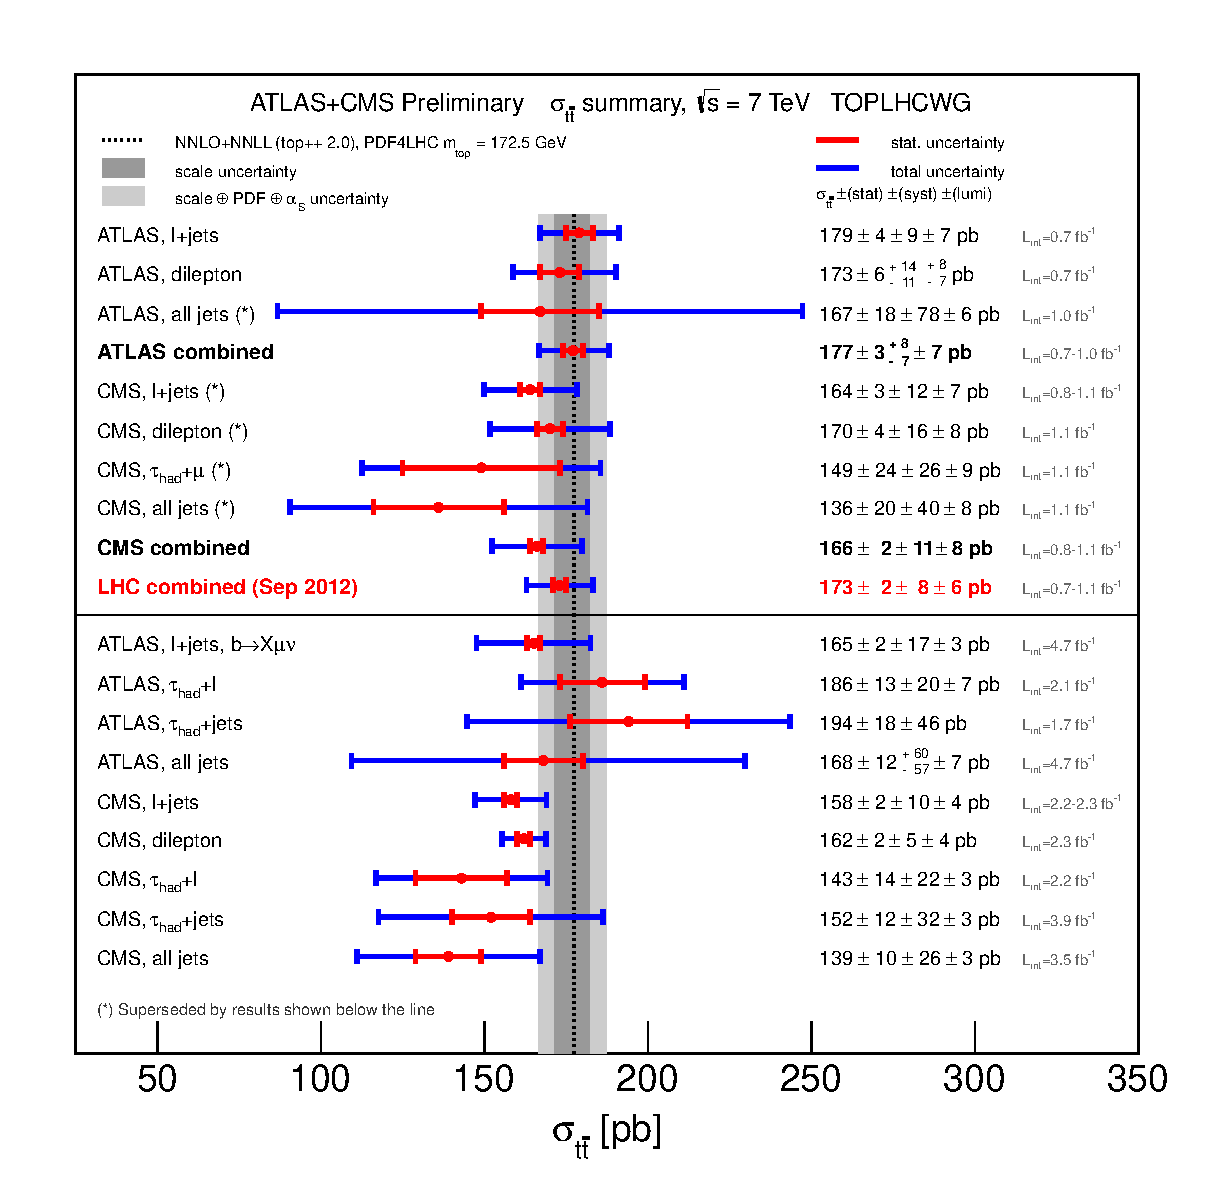
\includegraphics[width=0.95\textwidth]{PartTopQuark/Plots/tt_xsec_7TeV.eps}
  \caption{A summary of all \ttbar\ production cross section measurements performed at the LHC at $\sqrt{s}=7$ TeV. Note the theory prediction shown as a dotted black line with its associated uncertainties as grey bands. The results shown above the black line have been statistically combined, producing the results labelled as \textbf{combined}. Many of these analyses have been superseded and the results are shown below the line. Other analyses performed but not included in the combination are also shown below the line.}
  \label{fig:TopQuarkPairProductionSummaryLHC}
\end{figure}

\begin{figure}[htbp]
  \centering
  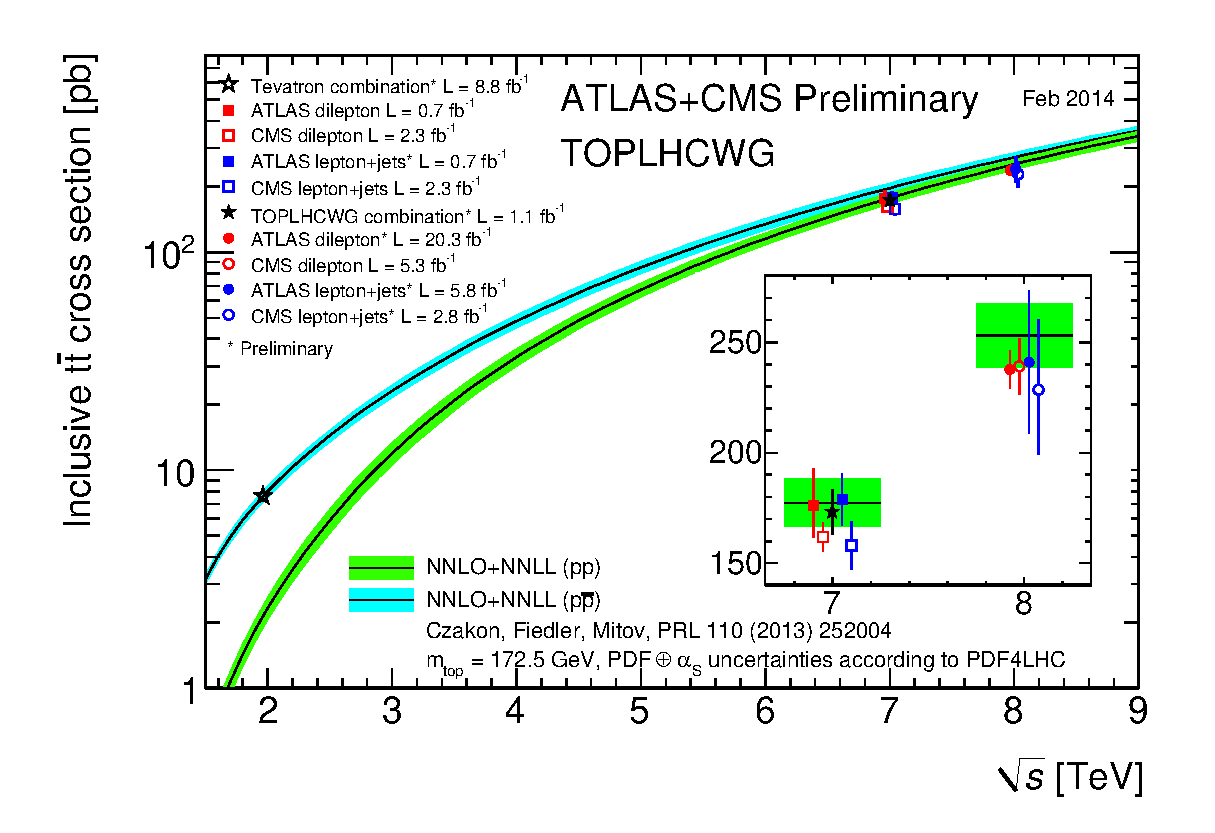
\includegraphics[width=0.95\textwidth]{PartTopQuark/Plots/tt_xsec_vsroots.eps}
  \caption{A summary of the most precise \ttbar\ production cross section measurements performed at the LHC at $\sqrt{s}=$ 7 and 8 TeV and the Tevatron at $\sqrt{s}=1.96$ TeV compared to the theoretical prediction. Note that the Tevatron results should be compared against the prediction for $p\bar{p}$ collisions while the LHC against the $pp$ collision predictions.}
  \label{fig:TopQuarkPairProductionComparison}
\end{figure}

\subsubsection{Mass asymmetry measurement}

As mentioned in Section~\ref{sec:TheoryWeakInteractions}, the charge ($C$) and parity ($P$) symmetries are both violated in weak interactions. The CPT symmetry which includes time reversal ($T$) is the last remaining symmetry which no interaction appears to violate. Any deviations from this symmetry would have major implications on particles physics~\cite{TopQuark:CPTViolation} and could manifest itself as differences between matter and antimatter particles. As the only quark which can be studied directly, measurement of $\Delta m\equiv m_{t}-m_{\bar{t}}$ could hint at any such deviation produced by new physics. Such a measurement was conducted by the ATLAS~\cite{TopQuark:MassAsymmetryATLAS2014} experiment yielding the result:
%
\begin{equation}
  \Delta m_{t}=-0.44\pm0.46\text{ (stat)}\pm0.27\text{ (stat) GeV}
\end{equation}
%
and by the CMS~\cite{TopQuark:MassAsymmetryCMS2012} experiment yielding the result:
%
\begin{equation}
  \Delta m_{t}=0.67\pm0.61\text{ (stat)}\pm0.41\text{ (stat) GeV}
\end{equation}
%
which are both consistent with the SM prediction and imply CPT invariance.

\subsubsection{Charge asymmetry}

Many BSM theories can affect the charge symmetry between top and antitop quarks. Once again any deviations from the SM prediction would point to the existence of new BSM physics. The charge asymmetry as measured by the ATLAS experiment~\cite{TopQuark:ChargeAsymmetryATLAS} is
\begin{equation}
  A_{c}=0.006\pm0.010
\end{equation}
%
and as measured by CMS~\cite{TopQuark:ChargeAsymmetryCMS}
%
\begin{equation}
  A_{c}=-0.010\pm0.017\text{ (stat)}\pm0.008\text{ (syst)}
\end{equation}
%
which once again are consistent with the SM prediction.



% !TEX root = ../Thesis.tex
\newcommand{\rphi}{\ensuremath{R-\phi}}
\newcommand{\T}{\ensuremath{\mathbf{T}}}
\newcommand{\Tms}{\ensuremath{\T_{\textrm{MS}}}}
\newcommand{\Tid}{\ensuremath{\T_{\textrm{ID}}}}
\newcommand{\C}{\ensuremath{\mathbf{C}}}
\newcommand{\Cms}{\ensuremath{\C_{\textrm{MS}}}}
\newcommand{\Cid}{\ensuremath{\C_{\textrm{ID}}}}

\chapter{The LHC and the ATLAS Detector} \label{sec:lhc_atlas_detector}

\section{The Large Hadron Collider} \label{sec:the_large_hadron_collider}

The Large Hadron Collider (LHC)~\cite{LHC} is a proton ring collider located at the European Centre for Nuclear Research (CERN). The main LHC ring is housed in the tunnel which previously contained the Large Electron-Positron collider. The LHC ring is \SI{27}{\kilo\meter} in circumference and located approximately \SI{175}{\meter} underground. The LHC services four different experiments located at four interaction points around the beam-pipe (Figure~\ref{fig:DetectorLHCLayout}). A toroidal LHC apparatus (ATLAS, the experiment used for this thesis), the compact muon solenoid (CMS), a large ion collider (ALICE) experiment and the LHC beauty (LHCb) experiment. 

ATLAS and CMS are general purpose detectors designed to support a varied physics programme, from SM physics like top quark measurements to BSM searches such as supersymmetry. ALICE and LHCb are more specialized experiments which focus on heavy ions and $b$ physics, respectively.

\begin{figure}[htbp]
  \centering
  \includegraphics[width=0.95\textwidth]{PartDetector/Diagrams/Cern-Accelerator-Complex.jpg}
  \caption{The layout of CERN complex of experiments, note the main four LHC experiments located at different points around the ring.}
  \label{fig:DetectorLHCLayout}
\end{figure}

The LHC accelerates two beams of protons in opposite directions and then collides the two beams at the four interaction points where the experiments are located. The protons come from hydrogen gas where the orbiting electron is removed by an electric field, leaving behind a bare proton. The beam acceleration occurs in several stages exploiting smaller experiments present at CERN. During 2010 and 2011 protons were accelerated to a beam energy of \SI{3.5}{\TeV}, creating a centre-of-mass energy of \SI{7}{\TeV} and then \SI{4}{\TeV} per beam in 2012 for a centre-of-mass energy of \SI{8}{\TeV}. Each beam is made of multiple bunches of protons, with as many as hundreds of billions of protons in each bunch. Bunches are grouped into \textit{bunch trains} with a designed \textit{bunch spacing} of \SI{25}{\ns} between each of the bunches that compose a single train. Note that the bunch spacing and size of the bunch can be altered to adjust the amount of collisions and the time between collisions. The variation in the number of colliding bunches is shown in Figure~\ref{fig:DetectorBunchesColliding}.

\begin{figure}[tbhp]
  \centering
  \begin{subfigure}[b]{0.95\textwidth}
    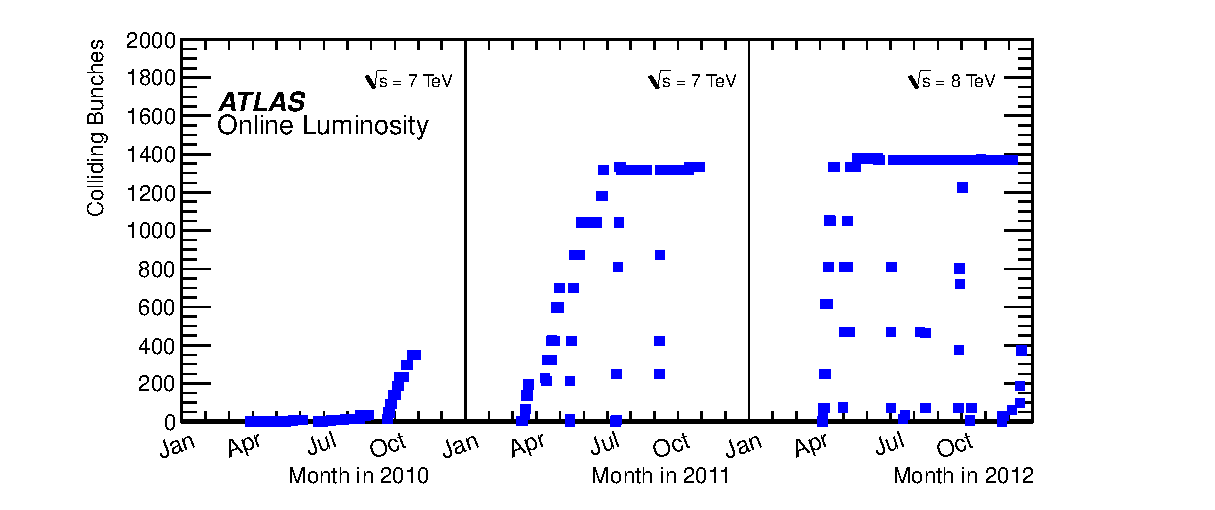
\includegraphics[width=\textwidth]{PartDetector/Plots/BunchesCollidingPerTime.eps}
    \caption{The number of bunches colliding per unit time at the LHC for the 2010, 2011 and 2012 $pp$ collision periods.} \label{fig:DetectorBunchesColliding}
  \end{subfigure}
  
  \begin{subfigure}[b]{0.95\textwidth}
    \includegraphics[width=\textwidth]{PartDetector/Plots/PeakLuminosityVsTime.eps}
    \caption{The peak luminosity per unit time at the LHC for the 2010, 2011 and 2012 $pp$ collision periods.} \label{fig:DetectorPeakLumi}
  \end{subfigure}
  \caption{Shown in \subref{fig:DetectorBunchesColliding} is the number of bunches colliding at the LHC and \subref{fig:DetectorPeakLumi} the peak luminosity per unit time.} \label{fig:DetectorPerformance}
\end{figure}

The acceleration of the proton beams occurs in several stages, within several different accelerators. The beams are first accelerated in a linear collider (LINAC 2) to an energy of \SI{50}{\MeV} before being injected into the proton synchotron booster (PSB). The beams are then boosted to \SI{1.4}{\GeV} by a varying magnetic field in the circular PSB. The beams are then passed into the proton synchrotron (PS) and then the super proton syncrotron (SPS) where the beam energy increases to \SI{26}{\GeV} and then \SI{450}{\GeV}. At this stage the beam is injected into the LHC and then accelerated to the final desired energy. The design energy is \SI{7}{\TeV} per beam for a total of \SI{14}{\GeV} centre-of-mass energy. From injection of the protons into LINAC 2 to stable beam conditions in the LHC, the whole process can take a couple of hours.

As bunches overlap the protons that make up the bunches interact, these interactions are known as events. The number of events is proportional to the instantaneous luminosity $\Lagr$ of the collider. $\Lagr$ is a measure of the flux of particles per unit area per unit time can be defined as:

\begin{equation}
  \Lagr=f{n_b}\frac{N_1 N_2}{A}
\end{equation}
%
where $f$ is the frequency of revolution of the beam, $n_b$ the number of colliding pairs of bunches in the beam, $N_1$ and $N_2$ are the number of particles in each colliding bunch and A is the cross-section of the beam~\cite{Luminosity}. The peak luminosity evolution at the LHC is shown in Figure~\ref{fig:DetectorPeakLumi}. Note that the operational $\sqrt{s}$ of the LHC was \SI{7}{\TeV} for 2010/11 and \SI{8}{\TeV} for 2012.

The total amount of data collected is measured by the integrated luminosity $\Lagr_{\textrm{int}}$ defined as the time integral of $\Lagr$. Integrated luminosity has units of inverse area, usually expressed in terms of barns (b)\footnote{1 $b^{-1}$ = $10^{-28}$ $m^{-2}$}. The probability for a given process to occur is expressed as the cross-section $\sigma$ and the total number of events which proceed via said process is defined as:
%
\begin{equation}
  \sigma\int\Lagr\,\mathrm{d}t
\end{equation}

The integrated luminosity delivered by the LHC and collected by the ATLAS detector in 2011 and 2012 is shown in Figure~\ref{fig:DetectorIntLumi}. The ATLAS detector does not record all data delivered by the LHC; approximately $6.5\%$ was not recorded.

\begin{figure}[htbp]
  \centering
  \includegraphics[width=0.65\textwidth]{PartDetector/Plots/IntegratedLuminosity20112012.eps}
  \caption{Distribution of the total integrated luminosity delivered by the LHC and the recorded by ATLAS for the 2011 and 2012 $pp$ collision period. Note the $\sqrt{s}$ changing from \SI{7}{\TeV} to \SI{8}{\TeV} between 2011 and 2012.}
  \label{fig:DetectorIntLumi}
\end{figure}

\subsection{Pileup}

Due to the large number of interactions and the short time between collisions, multiple events can overlap into a single event. This has detrminetal effects on physics analyses and is a determining factor in setting the instantenous luminosity with which to perform data collection. This overlapping effect is collectively known as pileup and is categorized into two types: in-time pileup, where multiple $pp$ collisions occur during the same bunch crossing; and out-of-time pileup, where the electric signals produced by a previous collision is still present in the detector. The number of interactions per crossing $\mu$ is shown in Figure~\ref{fig:DetectorBunchCrossingInteractions}, note that on average approximately thirty interactions occurred per bunch crossing in 2012. In comparison, in 2011 the average interactions per bunch crossing $<\mu>$ varied from $<\mu>=5$ in early 2011 to $<\mu>=15$ at the end of the year. The large number of overlapping events has a detrimental effect on physics analyses and thus is an important factor when setting the operational $\Lagr$ of the collider.

\begin{figure}[htbp]
  \centering
  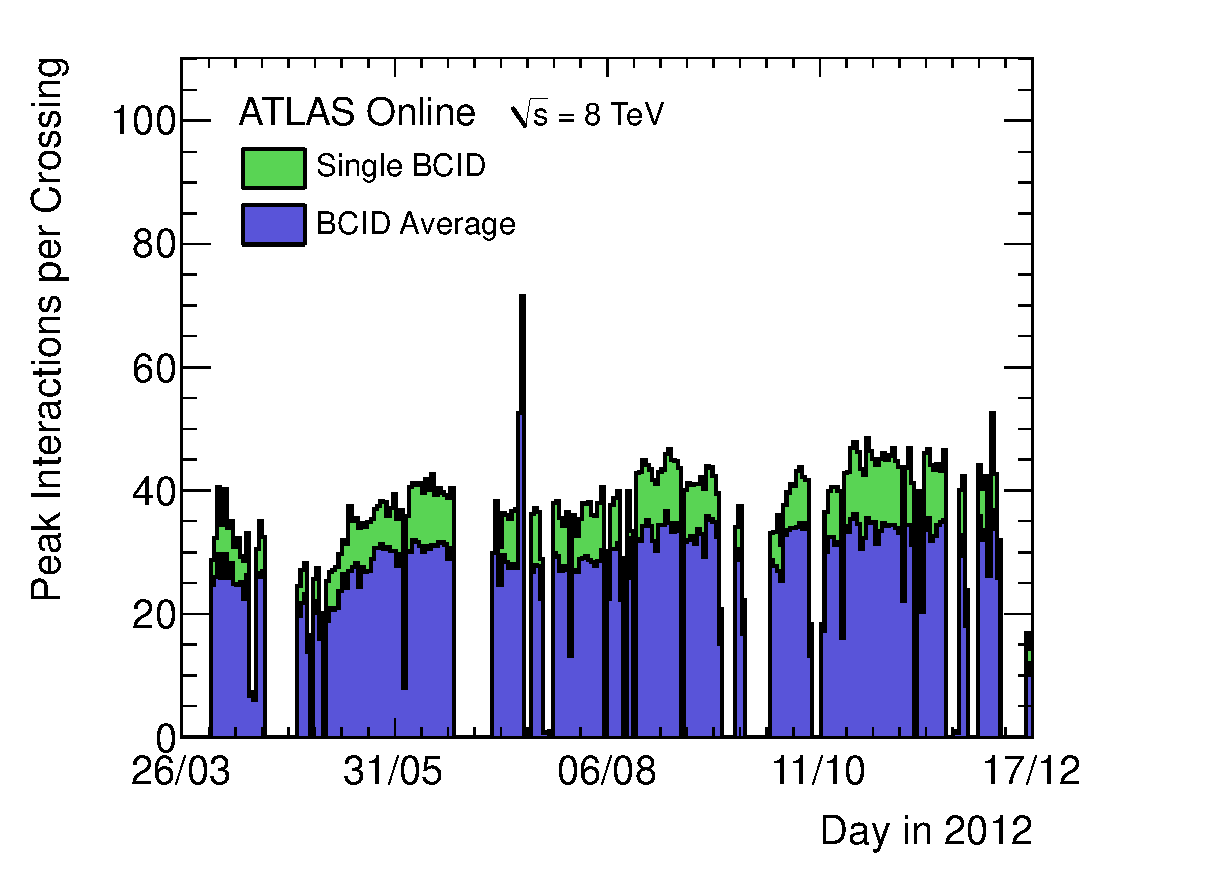
\includegraphics[width=0.65\textwidth]{PartDetector/Plots/peakBothMuByDay.eps}
  \caption{Number of interactions per bunch for the 2012 $pp$ data-taking period at ATLAS per day. Note that both the average number of interactions for all bunches and the maximum number of interactions are shown.} \label{fig:DetectorBunchCrossingInteractions}
\end{figure}

\section{The ATLAS detector} \label{sec:the_atlas_detector}

The ATLAS~\cite{Detector:ATLASExperimentGeneral} experiment is a general-purpose detector which wraps around the IP providing large angular coverage. ATLAS is approximately cylindrical with a diameter of \SI{25}{\meter}, a total length of \SI{44}{\meter} and weighs \SI{7000}{\tonne}. The detector is made of several layers of instrumentation located at succesively increasing radii as shown in Figure~\ref{fig:ATLASOverviewFigure}:

\begin{enumerate}
  \item \textbf{Inner Detector}: Located nearest to the beam-pipe and designed to measure the track of charged-particles.
  \item \textbf{EM Calorimeter}: Used for identification and measurement of electrons and photons.
  \item \textbf{Hadronic Calorimeter}: Used for the measurement of hadronic activity from hadronizing partons and missing transverse energy.
  \item \textbf{Muon Spectrometer}: The outermost detection layer, used for muon identification and measurement.
\end{enumerate}

Between these detection layers are magnets responsible for bending the path of the charged particles for the purpose of momentum measurement and particle identification. Additionally triggering and data acquisition (DAQ) systems form part of the detector for the purposes of recording the data signals coming from the aforementioned tracking and measurement systems. A brief description of these systems is provided in the coming sections. For a more detailed technical description of the detector and all subsystems see~\cite{Detector:ATLAS_TDR_vol1}.

Semi-leptonic \ttbar\ events produce a final state that includes hadronic activity, electrons, muons and missing energy and thus all elements of the detector are used in the reconstruction of such events. Additionally the match \xsm-tagger which is central to this thesis relies on the reconstruction and fitting of inner detector tracks and muon spectormeter tracks. A detailed description of this algorithm is provided in the Chapter~\ref{ch:CrossSection}. 

\begin{figure}[htbp]
  \centering
  \includegraphics[width=0.85\textwidth]{PartDetector/Diagrams/ATLAS_Overall.eps}
  \caption{An overview diagram of the ATLAS experiment. Shown are all detection and tracking systems and the toroid magnet which encompasses them. Note also the muon system on the outside of the detector.}
  \label{fig:ATLASOverviewFigure}
\end{figure}

A cylindrical coordinate system as used by all ATLAS publications has been adopted here. The coordinate system is constructed so that the $z$-axis is parallel to the beam axis. The $x$-axis is positive in the direction going from the IP to the centre of the LHC ring, and the positive $y$-axis points upwards. Thus the $x-y$ plane is transverse to the beam direction. All transverse variables such as the transverse momentum \pt, transverse energy \Et\ and missing transverse energy \met\ are measured along this plane. The azimuthal angle $\phi$ is measured around the beam axis, and the polar angle $\theta$ is the angle from the beam axis. The pseudorapidity is defined as $\eta=-\ln\tan(\theta/2)$. The distance in the $\phi$-$\eta$ plane between two objects is denoted by $\Delta R$ and defined as $\Delta R = \sqrt{\Delta\phi^{2} + \Delta\eta^{2}}$. Finally side A of the detector is defined as the positive $z$ side and side C is the negative $z$.

\subsection{Inner Detector} \label{subsec:DetectorID}
The inner detector (ID) is a tracking detector located closest to the beam-pipe and used for momentum and impact parameter measurement, vertex and track reconstruction and particle identification. The ID is designed to provide hermetic, high-resolution tracking in the range $|\eta|<2.5$. All components of the ID subsystem are shown in Figure

\begin{figure}[htbp]
  \centering
  \includegraphics[width=0.65\textwidth]{PartDetector/Diagrams/ATLAS_ID.eps}
  \caption{caption}
  \label{fig:DetectorIDOverview}
\end{figure}

The entire ID is contained within the central solenoid (CS) that generates a \SI{2}{\tesla} magnetic field for the purpose of momentum measurement. The trajectory of a charged particle is bent in the presence of a magnetic field. The str by a magnitude dependent on the momentum of the particle. By reconstructing this trajectory the momentum can be measured. 

The reconstruction of interaction vertices is of paramount importance, particularly when considering the large amount of pile-up observed at ATLAS. Interaction vertecies are reconstructed by fitting all reconstructed tracks to a point. The primary vertex (PV) is then defined as the vertex with the largest amount of momentum associated with it. In addition the reconstruction of secondary interaction vertecies is used for the identification of short-lived particles such as $B$-hadrons and $\tau$.

\begin{figure}[htbp]
  \centering
  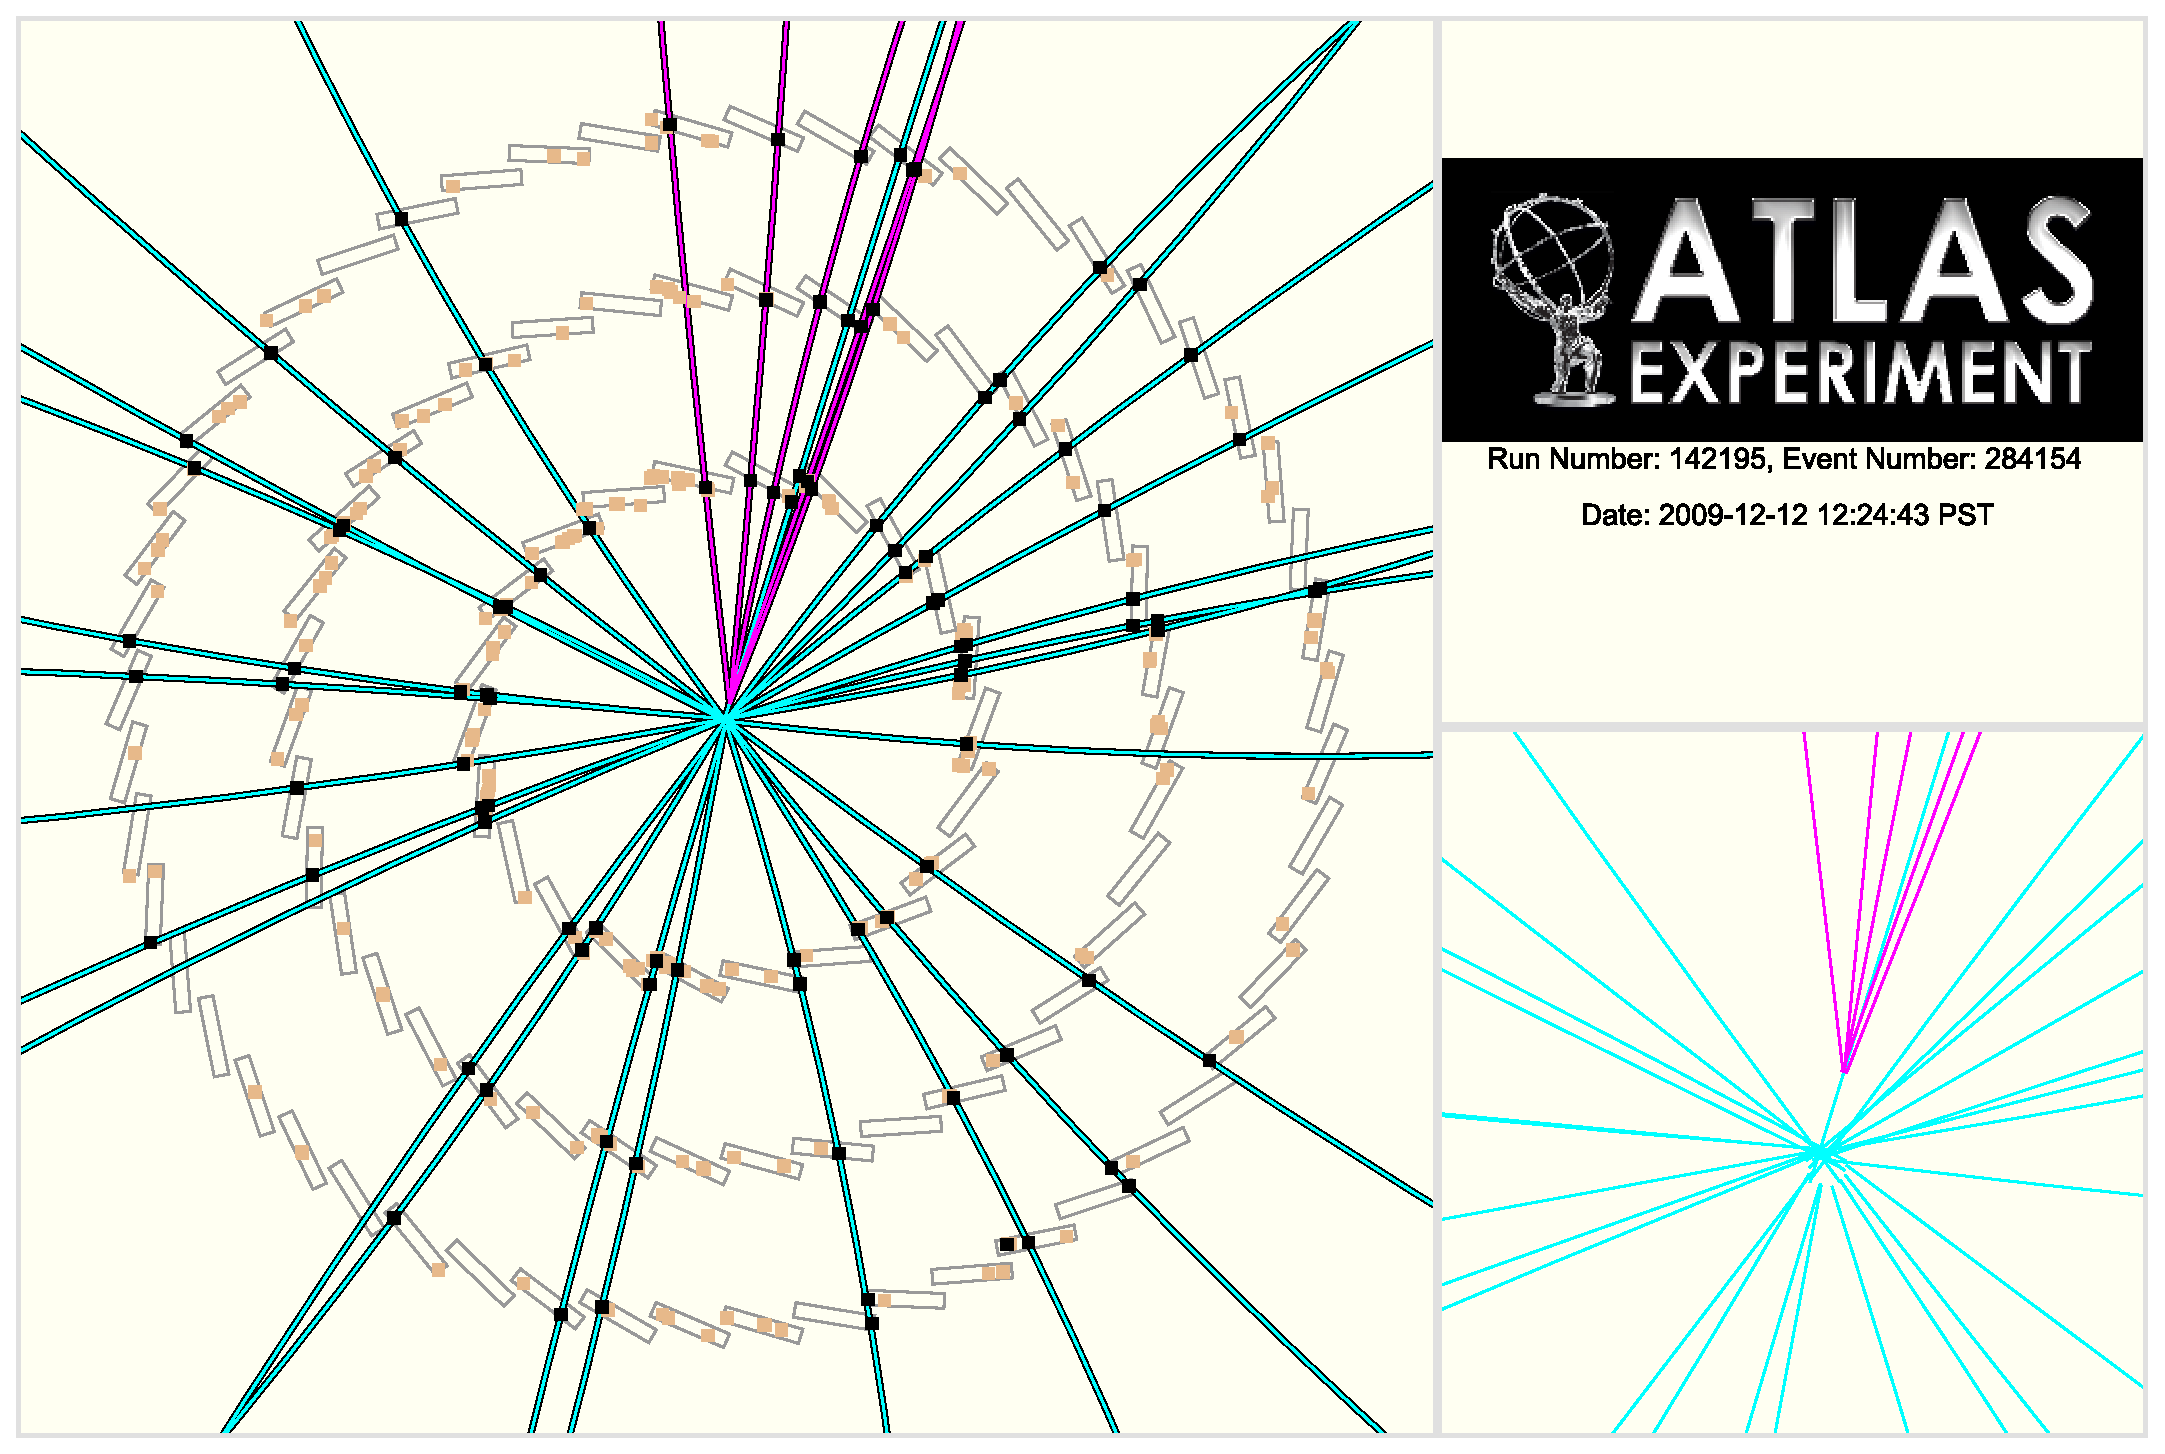
\includegraphics[width=0.95\textwidth]{PartDetector/Diagrams/fig_14.eps}
  \caption{An event-display of an event as reconstructed by the ATLAS inner detector. Shown are the results of the vertexing algorithm where each line represents a track. the purple tracks have been fitted to a secondary vertex.}
  \label{fig:label}
\end{figure}

The ID is made of three separate tracking and detection systems located at increasing radii away from the beam-pipe, the full arrangement can be seen in Figure~\ref{fig:DetectorIDQuarter} and a plane-view is shown in Figure~\ref{fig:DetectorIDTransverse}.

\begin{figure}[htbp]
  \centering
  \includegraphics[width=0.75\textwidth]{PartDetector/Diagrams/Detector_ID_QuarterView.eps}
  \caption{Plan-view of a quarter-section of the ATLAS ID showing the major detector elements with its active dimenstions and envelopes. Note also the $\eta$ markers showing the maximum coverage up to $\eta=2.5$.}
  \label{fig:DetectorIDQuarter}
\end{figure}

\begin{figure}[htbp]
  \centering
  \includegraphics[width=0.75\textwidth]{PartDetector/Diagrams/ID_3D_Overview.eps}
  \caption{A drawing of in the transverse plane of the ATLAS ID showing all major detection elements in the barrel regions. Note the charged particle track marked in red traversing all the detector elements.}
  \label{fig:DetectorIDTransverse}
\end{figure}

\subsubsection{Pixel detector}
The pixel detector is located nearest to the beam-pipe and provides high-granularity and precision for secondary vertex reconsruction. It consists of three silicon pixel sensors layers in the barrel region located at approximately \SIlist{5;9;12}{\cm} from the IP, and three disks at each side located at constant $R$ providing coverage up to $|\eta|<2.5$. The barrel modules are overlapped in a turbine pattern to provide hermetic coverage. In the barrel region the modules provide an intrinsic resolution of \SI{10}{\um} in \rphi\ and \SI{115}{\um} in $z$. The disk sections have an intrinsic resolution of \SI{10}{\um} (\rphi) and \SI{115}{\um} ($R$).

\subsubsection{Semiconductor tracker}
The semiconductor tracker (SCT) located in the intermediate radius range is designed to provide eight hits per track contributing to the measurement of momentum, impact parameter and vertex position. The SCT is made of four layers of stereo-pair silicon micro-strip sensors in the barrel region at increasing radii with an intrinsic resolution of \SI{17}{\um} (\rphi) and \SI{580}{\um} ($z$). At the end-caps nine disks of silicon microstrip modules provide large $\eta$ coverage with a resolution of \SI{17}{\um} (\rphi) and \SI{580}{\um} ($R$).

\subsubsection{Transition radiation tracker}
The transition radiation tracker (TRT) is the outermost tracking layer that forms the inner detector. The TRT is designed to provide up to 36 hits per track using straw-tube sensors. In the barrel the \SI{144}{\cm} long straw-tubes are arranged in modules which contain between 329 and 793 straws. The end-cap disks are made of radially distributed \SI{36}{\cm} long straw-tubes. Each straw-tube provides an intrinsic resolution of \SI{130}{\um} along its length. The combination of a large number of hits over a large radius allows for measurements in the TRT to be made with an accuracy that can complement those made by the pixel detector.

\subsection{Calorimetry}
The ATLAS calorimeter is responsible for the measurement of the energy of particles that emerge from the event. Sampling calorimeters are used for this purpose, layers of absorber material (passive) are placed in the path of the particles forcing them to interact and shower. The amount of energy lost by the incident particle depends on the type of material the particle traverses, the energy of the particle and the type. At high energies electrons lose energy predominantly via Bremsstrahlung, while photons lose energy via pair production. The characteristic length associated with this energy loss is a material characteristic known as the radiation length $X_0$.

For electrons the energy as a function of material traversed is 
%
\begin{equation}
  E=E_0e^{-x/X_0}
\end{equation}
%
where $E$ is the energy of the incident particle, $E_0$ is the original energy and $x$ is the distance traversed. As an electron traverses one $X_0$ of material, its energy is reduced by a factor of $1/e$. For photons the average number of photons traversing through a material length $x$ is reduced exponentially by a factor of $\frac{7}{9}X_0$.

The energy of the resulting shower is then measured by some sampling material (active) located behind the absorbers, this energy is proportional to the energy of the incident particle.

The type and thickness of material used is varied through the pseudorapidity range to improve energy measurement and reduce punch-through of particles into the muon systems behind. Due to the large amount of intense radiation produced during collisions, radiation hardness is also a driving factor in material choice.

The ATLAS calorimeter consists of the electromagnetic (EM) calorimeter, designed to measure photons and electrons covering the pseudorapdity region $|\eta|<3.2$; the hadronic calorimeter (HCal), designed to measure hadronic activity covering the pseudorapdity region $|\eta|<3.2$; and the forward calorimeter (FCal) which provides energy measurement capability in the very high pseudorapidity region $3.1<|\eta|<4.9$. As can be seen in Figure~\ref{fig:ATLASCalorimetryOverall} the calorimetry envelopes the ID and CS providing hermetic coverage symmetric in $\phi$. This is particularly important for the measurement of \met\ resulting from weakly interacting particles escaping the detector.

\begin{figure}[htbp]
  \centering
  \includegraphics[width=0.75\textwidth]{PartDetector/Diagrams/ATLAS_Calorimetry.eps}
  \caption{A cut-away diagram of the ATLAS detector highlighting the calorimetry system. Shown are the ECal barrel and end-cap, the HCal barrel and end-cap and the FCal end-cap.}
  \label{fig:ATLASCalorimetryOverall}
\end{figure}

\subsubsection{Electromagnetic calorimeter}
The EM calorimeter is made of a barrel section ($|\eta|<1.475$) and two end-caps ($1.375<|\eta|<3.2$). The EM barrel consists of two half-barrels separated by a \SI{4}{\mm} gap at $z=0$. The end-caps consist of two coaxial wheels, the outer ring covering the pseudorapidity range $1.375<|\eta|<2.5$ and the inner ring covering the range $2.5<|\eta|<3.2$. The pseudorapidity region $1.37<|\eta|<1.52$ is not used for precision physics due to the large amount of material, this is known as the ``crack'' region.

The EM calorimeter employs liquid Argon (LAr) as the active material due to its intrinsic radiation hardness and response over time, and lead as the passive material arranged in an accordion geometry for full $\phi$ symmetry. Particles interact with the lead absorbers creating a shower which ionizes the layers of liquid Argon. A potential is applied across the LAr material allowing for signal readout via Kapton/copper electrodes. The total thickness of the EM calorimeter is $>24X_{0}$ in the barrel and $>26X_{0}$ in the end-caps. The amount of material is optimized in pseudorapidity to enhance energy resolution.

In the region devoted to precision physics the EM calorimeter is divided into three segments as shown in Figure~\ref{fig:DetectorECalSegment}, the strip layer is designed to improve particle identification and pseudorapidity position measurement. The design energy resolution for all components of the calorimeter are shown in Table~\ref{tab:DetectorCaloResolution}.

\begin{table}
  \centering
  \caption{Design energy resolution of all ATLAS calorimeter components. The resolution is made of a sampling term ($\nicefrac{1}{\sqrt{E}}$) associated with the choice of passive and active materials and construction of the layers and a constant term associated with the depth of the detector, cracks and dead material.} \label{tab:DetectorCaloResolution}
  \begin{tabular}{|l|c|}
    \hline
    Section & Resolution \\
    \hline \hline
    EM Barrel & $\frac{10\%}{\sqrt{E}}\oplus0.7\%$ \\
    EMEC & $\frac{10\%}{\sqrt{E}}\oplus0.7\%$ \\
    HEC & $\frac{100\%}{\sqrt{E}}\oplus10\%$ \\
    FCAL & $\frac{100\%}{\sqrt{E}}\oplus10\%$ \\
    \hline
  \end{tabular}
\end{table}

\begin{figure}[htbp]
   \centering
   \includegraphics[width=0.75\textwidth]{PartDetector/Diagrams/LARG3-TDR-barrelM.pdf}
   \caption{Cut-away diagram of the EM calorimeter barrel at $\eta=0$. Shown are the three different layers with varying cell structures. The strip section is designed to enhance particle identification and position measurement in $\eta$.}
   \label{fig:DetectorECalSegment}
 \end{figure} 

\subsubsection{Hadronic calorimeter}
The hadronic calorimeter uses different types of passive and active material to accomodate for the varying conditions in different regions of the detector. The materials used and structure of the detector must provide good energy resolution, full symmetric coverage for the purpose of \met\ measurement,  full containment of all hardonic activity to prevent punch-through to the muon system and be sufficiently radiation hard.

The hadronic calorimeter consists of two parts a scintilator tile calorimeter in the barrel region, and a LAr calorimeter in the end-cap.

The tile calorimeter is located directly outside the EM calorimeter. The barrel portion of the calorimeter covers the region $|\eta|<1.0$ and the two extended barrels cover the range $0.8<|\eta|<1.7$. The tile calorimeter uses steel as the passive material and scintillating tiles as the active material. The resultingh hadronic showers enter the scintillating tiles and produce photons which are passed to photomultiplier tubes (PMTs). The total detector thickness which is tile-instrumented is 9.7 interaction lengths ($\lambda$) at $\eta=0$.

The hadronic end-cap (HEC) uses LAr technology due to its radiation-hardness in this challening high pseudorapidity region. The HEC consists of two independent wheels per end-cap covering the range $1.5<|\eta|<3.2$ overlapping the tile calorimeter at low pseudorapidity range and the forward calorimeter located at high pseudorapidity.

\subsubsection{Forward calorimeter}

The forward calorimeter (FCal) is responsible for energy measurement in the very-high pseudorapidity range $3.1<|\eta|<4.9$ of both electromagnetic and hadronic activity. Due to the large amount of radiation in this $\eta$ region, LAr is employed as the active material. The FCal consists of three layers, the first made primarily of copper, designed mostly for the measurement of electromagnetic activity while the two outer tungsten layers are responsible for hadronic activity measurement.

\subsection{Muon spectrometer}

The muon spectrometer (MS) is the outer most layer of the ATLAS detector (Figure~\ref{fig:DetectorDrawingMuonSystem}) and is responsible for the precision measurement of \pt\ of charged-particles that pass-through the ATLAS calorimetry. Muon tracking performance is vital to the SMT tagger described in Section~\ref{sec:CrossSectionSMT}, as it relies on the precise reconstruction of muon tracks in the ID and MS. Inner detector tracks and Muon spectrometer tracks are fitted to form a \emph{combined} muon track, the quality of the fit is at the core of the SMT algorithm.

Due to their larger mass, muons tend to have a larger tranverse momentum and as such do not lose as much energy through the emission of photons in the calorimetry. As a result, muons tend to traverse the hadronic calorimeter and escape the detector volume. The muon system provides measurement of these particles up to $|\eta|<2.7$ and triggering up to $|\eta|<2.4$. Measurement of \pt\ is facilitated by the magnetic field generated by the large toroid magnet in the barrel region $|\eta|<1.4$ and two smaller end-cap magnets in $1.6<|\eta|<2.7$. In the transition region ($1.4<|\eta|<1.6$) deflection is provided by the barrel and end-cap fields. 

\begin{figure}[htbp]
  \centering  
  \includegraphics[width=0.95\textwidth]{PartDetector/Diagrams/ATLAS_MuonSystem.eps}
  \caption{Cut-away drawing of the ATLAS muon system.}
  \label{fig:DetectorDrawingMuonSystem}
\end{figure}

The structure of the MS is delimited by the magnet system. In the barrel region three cylindrical layers of precision-tracking chambers are located in and on the coils of the barrel toroid magnet at radii of ~\SIlist{5;7.5;10}{\meter}. End-cap region coverage is provided by three chamber planes perpendicular to the $z$-axis located in front and behind the end-cap toroid magnet at distances $|z|\approx$~\SIlist{7.4;10.8;14;21.5}{\meter} from the interaction point.

The MS contains four different types of chambers responsible for precision-tracking and/or triggering in various pseudorapidity ranges as shown in Table~\ref{tab:DetectorMSOverview}. The arrangement of these chambers is shown in Figure~\ref{fig:DetectorMuonOverview}. 

\begin{table}
  \centering
  \begin{tabular}{|l|c|}
    \hline
    \textbf{Monitored drift tubes} & \textbf{MDT} \\
    - Coverage                     & $|\eta|<2.7$ (innermost layer: $|\eta|<2.0$) \\
    - Number of chambers           & 1150 \\
    - Function                     & Precision tracking \\
    \hline
    \textbf{Cathode strip chambers} & \textbf{CSC} \\
    - Coverage                      & $2.0<|\eta|<2.7$ \\
    - Number of chambers            & 32 \\
    - Function                      & Precision tracking \\
    \hline
    \textbf{Resistive place chambers} & \textbf{RPC} \\
    - Coverage                        & $|\eta|<1.05$ \\
    - Number of chambers              & 606 \\ 
    - Function                        & Triggering, second coordinate \\
    \hline
    \textbf{Thin gap chambers}        & \textbf{TGC} \\
    - Coverage                        & $1.05<|\eta|<2.7$~(2.4 for triggering) \\
    - Number of chambers              & 3588 \\
    - Function                        & Triggering, second coordinate \\
    \hline
  \end{tabular}
  \caption{Main parameters of the muon system.}
  \label{tab:DetectorMSOverview}
\end{table}

\begin{figure}[tbhp]
  \centering
  \begin{minipage}[b]{0.47\textwidth}
    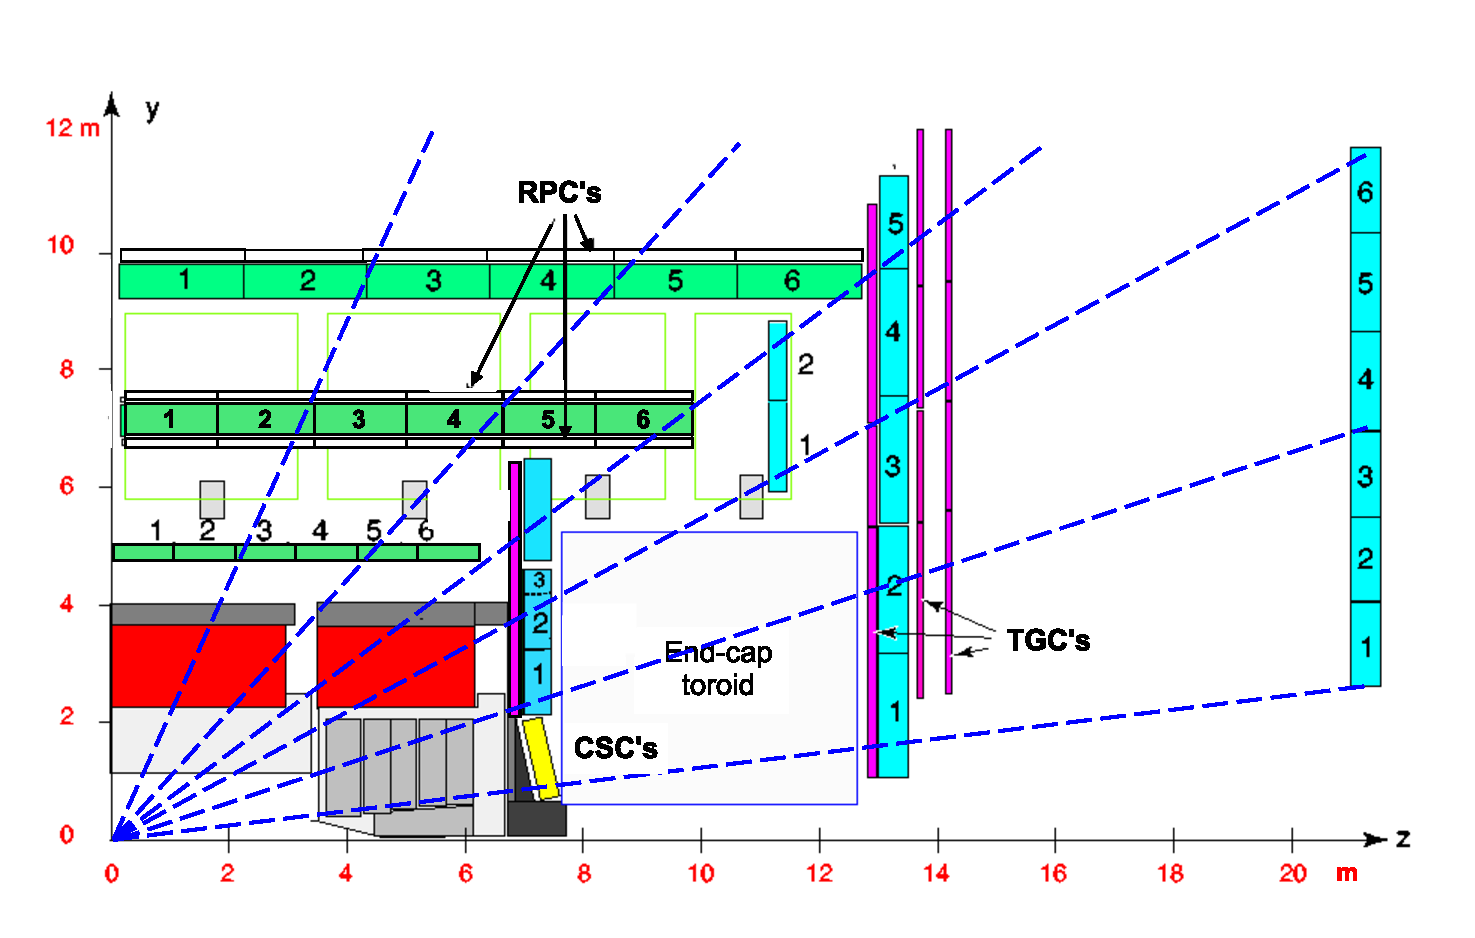
\includegraphics[width=\textwidth]{PartDetector/Diagrams/Muon_section.eps}
  \caption{Plan view of quarter-section of the ATLAS muon spectrometer.} \label{fig:DetectorMuonOverview}
  \end{minipage}
  \hfill
  \begin{minipage}[b]{0.47\textwidth}
   \includegraphics[width=\textwidth]{PartDetector/Diagrams/Muon_sector_numbering.pdf}
  \caption{Transverse view of the muon system. Shown are the } \label{fig:DetectorTransverse}
  \end{minipage}
\end{figure}

In the barrel region, precision-measurement is performed by monitored drift tubes (MDT) chambers. These chamber consist of three to eight pressuried aluminium drift tubes, each containing a tungsten-rhenium wire anode and a mixture of argon and carbon dioxide gas. An average spatial resolution of \SI{80}{\um} per tube and \SI{35}{\um} per chamber is achieved.

The end-cap region is instrumented with cathode-strip chambers (CSC) due to their higher rate capability and time resolution. CSCs are multiwire chambers with cathode planes segmented into strips in orthogonal directions. This allows for both coordinates to be measured simultaneously. The resolution of a chamber is \SI{40}{\um} in the bending plane ($R-z$) and \SI{5}{\mm} in the transverse plane.

Triggering on muon tracks is another essential role of the muon spectrometer. To this end, each precision-measurement chamber is complemented with fast triggering chambers. As with the measurement layers, two different types of chambers are used for the barrel and end-cap regions. In the barrel region ($|\eta<1.05$) resistive plate chambers (RPC) are used attached to the same support structure as the MDTs. The RPCs are made of two resistive plates, \SI{2}{\mm} apart, between which a potential difference is applied. The gap between the plates is filled with a mixture of $\textrm{C}_2\textrm{H}_2\textrm{F}_4$/Iso-$\textrm{C}_4\textrm{H}_{10}$/$\textrm{SF}_6$. The signal is read out via metallic strips mounted to the outer faces of the resistive plates. The end-cap region ($1.05<|\eta|<2.4$) is populated with thin gap chambers (TGC). TGCs multiwire chambers like those used in the CSC, however the distance between the wire and the cathode is smaller in the TGC. A summary of the spatial and temporal resolution for the measurement and triggering layers is shown in Table~\ref{tab:MSPerfomanceSummary}.
%
\begin{table}
  \centering
  \begin{tabular}{|c|c|c|c|}
   \hline
   Type & $R/z$ & $\phi$ & time \\
   \hline
   MDT & \SI{35}{\um} $(z)$ & -- & -- \\
   CSC & \SI{40}{\um} $(R)$ & \SI{5}{\mm} & \SI{7}{\ns} \\
   RPC & \SI{10}{\mm} $(z)$ & \SI{10}{\mm} & \SI{1.5}{\ns} \\ 
   TGC & \SIrange[range-phrase=-,range-units=single]{2}{6}{\mm} $(R)$ & \SIrange[range-phrase=-,range-units=single]{3}{7}{\mm} & \SI{4}{\ns} \\
   \hline
  \end{tabular}
  \caption{Summary of spatial and temporal resolutions per chamber for all chamber types used in the the ATLAS muon spectrometer. Adapted from~\cite{Detector:ATLASExperimentGeneral}.}
  \label{tab:MSPerfomanceSummary}
\end{table}

\subsection{Magnet system}
The structure of the ATLAS detector is defined by the large magnet system. The ATLAS magnet system, shown in Figure~\ref{fig:DetectorMagnet}, consists two sets of magnets. The central solenoid and three air-core toroids.

The central solenoid located nearest to the beam, provides a \SI{2}{\tesla} magnetic field for the ID for the purpose of tracking, particle identification and \pt\ measurement.

The barrel toroids extend to $|\eta|<1.4$ and are made of eight coils, generating a \SI{0.5}{\tesla} magnetic field for the MS. In the high pseudorapidity range, magnetic deflection is provided by two end-cap toroids extending from $1.6<|\eta|<2.4$. As in barrel, the end-cap toroids are made of eight coils offset by \SI{22.5}{\degree} with respect to the barrel coils. Each end-cap generates a \SI{1}{\tesla} magnetic field for the MS. The so-called transition region between the two magnets is covered by an overlap of the end-cap and barrel fields.

\begin{figure}[htbp]
  \centering
  \includegraphics[width=0.75\textwidth]{PartDetector/Diagrams/ATLcoilGeom.eps}
  \caption{Diagram of the ATLAS toroid magnet system. The red central solenoid is located closest to the beam surrounded by layers of tile calorimetry. The eight barrel toroid magnets are shown along with the offset end-cap toroids at each end.}
  \label{fig:DetectorMagnet}
\end{figure}

\subsection{Triggering and DAQ}

At the design luminosity of the LHC $\Lagr$=\SI{10e34}{\per\square\cm\per\second}, the expected event rate is approximately \SI{1}{\GHz}. At an average event size of \SI{1.3}{\mega\byte} per event, the total amount of data produced at ATLAS is \SI{1.2}{\peta\byte\per\second}. The maximum rate of data storage at ATLAS is approximately \SI{300}{\mega\byte\per\second}, so the rate must be reduced.

The trigger and data acquisition system (TDAQ) is responsible for selecting only ``interesting'' events for recording, thus reducing the rate. This is known as an \emph{online selection} as it happens before the data is stored. Selections during analysis for example, are known as \emph{offline selection}, as they happen after the data has been recorded.

The overwhelming majority of events produced at the LHC are of no interest to physics analysis, for example the so-called \emph{minimum bias events}. % Explain minbias

At ATLAS, trigger decisions are carried out in three sequential levels: \emph{Level 1} (L1), \emph{Level 2} (L2) and \emph{Event Filer} (EF), each successive level reduces the rate by applying increasingly more complex selection criteria. The hardware-based L1 trigger, performs the initial selection based on reduced-granularity information from the MS trigger chambers and all calorimeters. Data from the calorimeter trigger towers, shown in Figure~\ref{fig:DetectorECalSegment}, is used to search for presence of high transverse-momentum muons, photons, electrons, hadronic decays of $\tau$ leptons and hadronic jets, as well as large missing transverse energy and large total transverse energy. The central trigger processor applies the the trigger `menu' which includes a combination of selection criteria. Events which are of interest to physics analyses can be produced at such a rate as to overwhelm the capabilities of the DAQ. A \emph{prescale} can be applied to record one out of many of these events, thus reducing the rate. The L1 trigger also constructs \emph{regions of interest} (RoIs) around the detector where interesting features have been found. The $\eta$ and $\phi$ information of the RoI along with information about the decision is stored and passed to the higher level triggers.

The L2 selection makes use of RoIs and the full granularity of the detector to further reduce the event rate to approximately \SI{3.5}{\kHz} and finally the EF implements selections commonly used for offline analysis to reduce the rate to \SI{200}{\Hz}.

\section{Monte Carlo Simulation} \label{DetectorMC}

The simulation of data is paramount to HEP research, from the initial detector design phase all the way through to finalized analyses. Monte Carlo (MC) generators simulate various interactions, creating kinematic collision event data that reflect our best understanding of nature. These processes are then passed through detector simulation and all the object reconstruction algorithms, resulting in a dataset with an identical format to collision data. 

Simulation of data happens in three phases: event generation, detector simulation and digitization. 

\subsection{Event Generation} \label{DetectorEventGeneration}

Event generators are tools that model complex physics processes that occur during a particle collision. Many different generators exist to model a variety of beam types ($pp$, $p\bar{p}$, $e^+e^-$, etc...) and event types. Hadronic event generation simulates all components which make up the interaction, namely the hard scattering process, parton showering, hadronising, hadronic decay, the underlying event and photon radiation~\cite{Les} as shown in Figure~\ref{fig:DetectorEGSketch}.

\begin{figure}[htbp]
  \centering
  \includegraphics[width=0.85\textwidth]{PartDetector/Diagrams/scetch.eps}
  \caption{Sketch of a proton-proton collision as modelled by the event generator~\cite{Event}. Shown are the incoming protons beams as green arrows on the left and right sides of the diagram. The partons shown in blue, interact in the hard interaction (red blob) producing a parton shower, also depicted in red, which eventually hadronize (light green blobs) and finally decay into final state particles shown in dark green. The \emph{underlying event} is shown at the bottom of the diagram as the purple blob, note also the beam remnants as light blue blobs that also form part of the underlying event. Photon emission is shown in yellow and occurs at all stages of the event generation.}
  \label{fig:DetectorEGSketch}
\end{figure}

First, the \emph{hard interaction} of a pair of partons originating from the colliding protons is simulated. An example of such an interaction is $q\bar{q} \rightarrow Z / \gamma^{*}\rightarrow e^{+}e^{-}$. Calculating the cross section for such an interaction involves the convolution of the parton density function (PDF) and the \emph{matrix element} (ME).

The PDF $f_i(x,Q^2)$, describes the probability of finding, within the proton, a parton of flavour $i$ carrying a fraction $x$ of the proton momentum, via a hard interaction with energy scale $Q$. The ME describes the interaction between the two partons and corresponds to one or more of the feynman diagrams associated with the interaction\footnote{For a rigurous discussion of matrix elements and the Feynman rules, see~\cite{Theory:Perkins,Theory:IntroGriffiths}}. The order of a diagram is determined by the number of coupling constants associated with it. Different generators are capable of treating diagrams at different orders. The hard interaction is usually modelled at LO or NLO.

The next step is \emph{parton-showering} which simulates the  emission of gluons by coloured partons. A cascade of partons is produced, as shown in Figure~\ref{fig:DetectorEGSketch}, and modelled by perturbation theory for energies above \SI{1}{GeV}. All colored objects are then combined into colorless hadrons in a process known as \emph{hadronization}, these hadrons are subsequently allowed to decay.

Finally, the remaining colored partons not involved in the hard interaction, are allowed to interact forming the \emph{underlying event}.

The kinematic information of the original event without the effects of the detector is kept in the data set and is usually referred to as the \emph{truth information}.

\subsection{Detector simulation} \label{sec:DetectorSimulation}

The generated events are then passed through a detector simulation that mimmicks the response of the detector to particles traversing through it. A description of the entire detector is implemented in the GEANT4 toolkit, including a map of the magnetic fields, the position of the detector components and material description. The software then simulates the signal voltages produced in all tracking and calorimeter components of the detector, these are then passed through a simulation of the read-out electronics and DAQ taking into account known losses and inefficencies. All of this information is then passed on to the reconstruction software that ``rebuilds'' the physics objects from the detector \emph{hits}.

\section{Event reconstruction} \label{sec:DetectorEventReco}

The process of converting the raw data from the detector into formed events with physics objects (electrons, muons and so on) is known as \emph{event reconstruction}. The algortihms for object reconsruction are identical for both collision data and simulated data. The focus of this thesis, the soft muon tagger, is used on \emph{STACO combined} muons. Therefore some details of the muon reconstruction algorithms are discussed in the next section.

\subsection{Muon reconstruction} \label{sec:DetectorMuReco}

Muon reconstruction can make use of the information provided by both the inner detector and the muon spectrometer systems. Several muon reconstruction strategies exist~\cite{Detector:MuonReconstructionList}:

\begin{itemize}
  \item \textbf{Standalone reconstruction}: Uses MS information only, first constructing \emph{segments} from several hits in a given chamber and then fitting segments from all three stations to hits from the four MS components. Tracks are then extrapolated back to the IP taking into account energy loss and multiple scattering.
  \item \textbf{Tagging ID tracks reconstruction}: Uses MS or calorimeter information to tag ID tracks as muons.
  \item \textbf{Combined track reconstruction}: Standalone muon tracks are extrapolated back to the vertex and matched to ID tracks within ($|\eta|<2.5$) and combined. This results in an improved momentum sensitivity from ID and MS information. 
\end{itemize}

These strategies can be implemented in a variety of ways. There are two prominant families, STACO and MUID, that contain reconstruction packages which exploit one or a combination of these strategies. The STACO combined algorithm is used by the SMT tagger and is described in more detailed below.

\subsubsection{STACO Combined Algorithm} \label{sec:DetectorSTACO}
The STACO package combines ID and MS tracks by performing a statistical combination of the two independent tracks using track parameters ($\eta$, $\phi$, \pt, $d_{0}$, $z_{0}$) and their covariance matrices. The quality of the fit is represented in the resulting \xsm:
%
\begin{equation*}
  \xsm = (\Tms-\Tid)^T(\Cms+\Cid)^{-1}(\Tms-\Tid) \\
\end{equation*}
%
where \Tms\ and \Tid\ contain the track parameters for the MS track and the ID track respectively,
% 
\begin{equation*}
  \T_{\textrm{MS or ID}} =
  \begin{pmatrix}
    \eta \\
    \phi \\
    \pt \\
    d_{0} \\
    z_{0}
  \end{pmatrix}
\end{equation*}
%
and \Cms\ and \Cid\ are the covariance matrices, defined as
%
\begin{equation}
  \C_{ij} = (\T_i-\langle \T_i\rangle)(\T_j-\langle \T_j\rangle)
\end{equation}
%
where $\langle \T_i\rangle$ is the expectation value of $\T_i$. The full covarience matrix is included in Appendix~\ref{app:DetectorCov}.

If more than one possible combination per track exists, the best combined \xsm\ is chosen and then the track is removed from the pool of tracks to be match. The algorithm continues making associations until no more tracks remain.

\subsubsection{Soft Lepton Tagging} \label{sec:DetectorSLT}

\emph{Soft lepton tagging} (SLT) algorithms attempt to identify leptons produced in the semileptonic decay of $b$ and $c$ quarks for the purpose of determining the presence of HF quarks. The term ``semileptonic'' here refers to the decay of a $b$-hadron in such a way as to produce a lepton-neutrino pair along with an additional hadron. The lepton produced would have a low-\pt\ and as such as is known as a soft lepton. SMT tagger exploits muons and as such these will be the focus of the following discussion. 

A soft muon can be produced in a variety of ways starting with a $b$-quark, either directly via $b\rightarrow \mu\bar{\nu}_{\mu}X$, where $X$ is any hadron; or indirectly, via a $c$, $\bar{c}$ or a $\tau$ lepton. A summary of the BR for each of these decays is shown in Table~\ref{tbl:DetectorSLTBR}. The total BR for the production of a soft muon from a $b$ is \SI[multi-part-units=single,separate-uncertainty]{20.1(1)}{\percent}, thus the probability for a \ttbar\ event to contain atleast one semileptonically decaying $b$ is approximately \SI{38}{\percent}. The SMT tagger is described in detail in Section~\ref{sec:SMTExplanation}.

\begin{table}
  \centering
  \begin{tabular}{|l|c|}
  \hline
  Mode                                       & Muon BR \\
  \hline % -------------------------
  $b\rightarrow \mu$                         & $10.95^{+0.29}_{-0.25}~\%$ \\
  $b\rightarrow c \rightarrow \mu^{+}$       & $8.02\pm0.19~\%$ \\
  $b\rightarrow \bar{c} \rightarrow \mu^{-}$ & $1.6\pm0.5~\%$ \\
  $b\rightarrow \tau \rightarrow \mu$        & $0.42\pm0.04~\%$ \\
  \hline % -------------------------
  All modes                                  & $21.0\pm1.0~\%$ \\
  \hline % -------------------------
  \end{tabular}
  \caption{Branching ratio for the production of a muon from a $b$-quark in both direct and indirect modes~\cite{Theory:PDGBooklet}.} \label{tbl:DetectorSLTBR}
\end{table}

\chapter{Identifying $b$-jet, and the Match $\chi^{2}$ based Soft Muon Tagger} \label{prt:smt_summary}
This section will include a description of several current methodologies for b-jet tagging
and a detailed description of the Match-$\chi^{2}$ Soft Muon Tagger.
\section{$b$-jet tagging methodology} \label{sec:b_jet_tagging_methodology}
\section{The Match-$\chi^{2}$ Soft Muon Tagger} \label{sec:smt_tagger}

% !TEX root = ../Thesis.tex
\chapter[Calibration of the Soft Muon Tagger]{Calibration of the Soft Muon Tagger for 2012 ATLAS Data} \label{ch:Calibration}

High-energy physics relies heavily on the use of simulated data to inform the development of analysis techniques. It is thus paramount that the simulation reflect nature as closely as possible. However the simulation does not accurately predict conditions within the detector and the effects on the muon reconstruction and the quality of the fit between the inner detector tracks and muon spectrometer tracks which is represented in the \xsm. Instead the difference between simulation and data is quantified and taken into account. This process is known as calibration. In the case of the muon reconstruction method and the \xsm\ tagger it is important that the difference in efficiency between MC and data be accounted for. This is done by constructing a scale factor, defined in this case by:

\begin{equation}
  \kappa_{\textrm{\xsm}} = \frac{\epsilon_{\xsm}^{\textrm{Data}}}{\epsilon_{\xsm}^{\textrm{MC}}}
\end{equation}

One of the advantages of using the \xsm\ tagger over other forms of tagging is that the presence of a jet is not required to measure the \xsm\ of a muon. This means that the calibration can be performed on a isolated muons such as those from $\jpsi \rightarrow \mu\mu$ or $Z\rightarrow\mu\mu$ using the so called tag and probe method. This calibration relies on muons with low \pt\ from \jpsi\ decays. As the \xsm\ is a characteristic of combined and therefore reconstructed muons, 

The tag and probe method used in this calibration is defined as follows. One reconstructed combined muon is designated as the Tag, this muon must pass a stringent set of cuts implying that this is indeed a muon from a \jpsi. The second muon which is designated as the Probe is constructed from an inner detector (ID) only. To ensure that the Probe is the second muon from the \jpsi\ decay, the invariant mass of the combined tag and probe system is required to be within a mass window centered around the true \jpsi\ mass. The complete selection used in the calibration is detailed in Section~\ref{sec:CalibrationSelection}. These Probes are then used to measure the reconstruction efficiency and the \xsm\ tagger efficiency as described in Sections~\ref{sec:CalibrationFitting} and \ref{sec:CalibrationEfficiencies}.

The tag and probe method used here is based on a previous calibration of the \xsm\ tagger performed on 2011 ATLAS collision data outlined in %CITE OLD CALIBRATION NOTE.
This analysis differs from the 2011 calibration in several ways these will be highlighted and explained.

\subsection{Software, Collision Data and Simulated samples}
The tag and probe method used here was implemented using the \textsc{ROOT} analysis framework. 

The calibration was performed on a dataset made of those luminosity blocks selected by the recommended standard Good Runs List (GRL) which corresponds to all $pp$ collision periods in 2012. The GRL selects only those luminosity blocks where detector conditions are appropriate for physics data-taking. This includes all relevant detector components being operational and that stable beam conditions have been achieved.
The datasets are part of the 2013 summer reprocessing (processing tag p1328) corresponding to data taken in periods A through to L, excluding periods F and J. 

The efficiency scale factor is measured against a sample containing almost 10 million $\jpsi\rightarrow\mu\mu$ events. At event generation filters are applied so the sample only contains events where both muons have a transverse momentum of at least \SI{4}{\GeV} and they must lie within the pseudorapidity range $|\eta|<2.5$. This selection matches the object selection used by most analyses as recommended by the Muon Combined Performance (MCP) group. 

\section{Tag and Probe Selection} \label{sec:CalibrationSelection}

A tag and probe method was chosen to measure the efficiency of muon reconstruction and the \xsm\ tagger. The tag and probe method allows for the measurement of the performance of selection criteria or algorithms by exploiting well known decays. By creating a sample of objects, in this case muons, on which to apply the aforementioned selection criteria, it is possible to study these algorithms.

The muon reconstruction algorithm examines various Inner Detector (ID)tracks and Muon Spectrometer (MS) tracks and makes a determination as to whether said track is produced by muon or not. To measure the performance of the muon reconstruction algorithm a sample of ID tracks which originate from the \jpsi\ decay and are thus very likely to be a real muon is constructed. This is done in the following way:

First, require the presence of a combined \staco\ muon which passes a very stringent selection. This strongly implies that this is a real muon and thus is labelled as the Tag. Additionally a very loose selection is applied to all ID tracks. These are known as candidate Probes. Pairs of tag and probes are then formed by requiring that the combined invariant mass lie within a \jpsi\ mass window and the pair pass additional pairing cuts. This then implies that the Probe is likely the other muon from the \jpsi\ decay and as such is a suitable test-bed to measure the performance of the muon resconstruction algorithm. Note that all selection criteria are detailed and explained in Section~\ref{sec:CalibrationSelectionCuts}

After selecting a sample of probes the performance of the algorithm is estimated by measuring the proportion of probe candidates which are selected by the algorithm. In other words the performance is estimated by counting the number of muons which are reconstructed given that the ID track is very likely to be a real muon. Probes which are reconstructed into combined \staco\ muons are labelled as muon probes. The performance of the \xsm\ tagger is estimated in a similar manner, by measuring the proportion of combined muon probes which pass the SMT selection.

\subsection{Trigger requirements} \label{sec:CalibrationTriggerRequirement}
In order for an event to be included in the analysis it must pass at least one of the trigger chains listed in Appendix~\ref{app:CalibrationTrigger}. For the sake of brevity only the primary trigger (\verb|EF_mu6_Trk_Jpsi_loose|) which contributes the majority of events is described here.

As stated in the trigger name this is an Event Filter trigger which requires the presence of a muon with a momentum of at least \SI{6}{GeV} and an ID track whos combined invariant mass lies within a \jpsi\ mass window of \SI{2.6}{GeV}<$m_{\textrm{inv}}$<\SI{3.6}{GeV}. This loose mass window contains the entirety of the \jpsi\ peak in all examined \pt\ and $\eta$ ranges as well as additional side bands to allow for background removal. Note the omission of double muon triggers to avoid introducing a bias by specifically selecting events with two good muons. 

Also note that while all triggers are operational in all periods, most are heavily prescaled and the prescale is period dependent. This does not have a first-order effect on the measurement since only ratios are compared between collision data and MC.

\subsection{Selection Cuts} \label{sec:CalibrationSelectionCuts}
The selection criteria for tags, probes, muon probes and SMT muons are listed and detailed below. Note that all cuts are applied on the kinematic properties measured in the ID due to its improved resolution unless it is not possible as in the case of the \xsd\ which is a combined MS and ID property. Also note that all objects must pass a selection criteria collectively refered to as MCP cuts. These are tracking quality cuts which require a certain number of detector elements be active to ensure good tracking. These cuts are listed in 

The muon tag selection criteria are defined in the list below:

\begin{itemize}
  \item MCP cuts
  \item \staco\ collection
  \item Combined muon
  \item $\pt$>\SI{4}{\GeV}
  \item $|\eta|$<2.5
  \item $|d_{0}|$<\SI{0.3}{\mm} and $|z_{0}|$<\SI{1.5}{\mm}
  \item $|d_{0}/\sigma_{d_{0}}|$<3 and $|z_{0}/\sigma_{z_{0}}|$<3
  \item Fired at least one of the relevant triggers (see Appendix~\ref{app:CalibrationTrigger})
\end{itemize}

Included are cuts on the muon impact parameter (IP) $d_{0}$ and $z_{0}$. These are defined as the distance of closest approach of the ID track to the primary interaction vertex in the transverse and longitudinal planes, respectively. Additionally cuts on the absolute values of IP significances are also implemented. The signifiance of the impact parameter is defined as $d_{0}/\sigma_{d_{0}}$ where $\sigma{\textrm{IP}}$ is the standard deviation of the impact parameter. These cuts are designed to ensure that the muon selected originates near the primary vertex and thus from a prompt \jpsi\ from the primary collision. Note that non-prompt \jpsi\ can be produced in the decay of $b$ hadrons. Finally note that the tag muon must match the trigger object which selected this event.

The probe selection is a subset of the tag selection and only requires an ID track with $|\eta|<2.5$ and $\pt>$\SI{4}{\GeV}. The pairing cuts are shown below:

\begin{itemize}
  \item \SI{2}{\GeV}$\leq m_{\textrm{inv}}\leq$\SI{4}{\GeV}
  \item Probe charge is opposite the tag charge 
  \item 0.4<$\Delta$R(tag, probe)<3.5
  \item $\Delta z_{0}$(tag, probe)<\SI{0.2}{\mm}
\end{itemize}

The probe and the tag are required to be fairly well separated to avoid the momentum of the tag from entering the isolation cone of the probe. In the 2011 calibration analysis the track of the tag and the probe are refit to a common vertex and the quality of the refit, expressed by the $\chi^2$ is a part of the pairing criteria. This criteria is present to reduce the effects of pile-up on the measurement, by ensuring both objects have a common origin. Since the data format used for this analysis is a derived form of that used in 2011 it is not possible to perform such a refit. Instead the difference between the $z_{0}$ of the tag and the probe is used.

The \staco\ reconstruction efficiency is not measured by applying the algorithm on the probe collection but rather a probe is said to be a muon probe if it matches a combined muon from the \staco\ collection. This is done by requiring the angular separation between the probe and the \staco\ muon be less than 0.001. Probes which are matched become the numerator of the reconstruction efficiency and the denominator is defined as the number of probes:

\begin{equation*}
  \epsilon = \frac{N_{\textrm{muon probe}}}{N_{\textrm{probe}}}
\end{equation*}

A muon probe is said to be an SMT muon if it passes the following selection, which matches the muon cuts defined in Section~\ref{sec:CrossSectionSMT}. Note in particular the main component of the soft muon tagger, the cut on $\xsm/N_{\textrm{dof}}<3.2$, the distribution of the \xsd\ is shown in Fig.~\ref{fig:CalibrationMatchChi2Dist} 

\begin{itemize}
  \item $|d_{0}|$<\SI{3}{\mm}
  \item $|z_{0}\sin(\theta)|$<3
  \item $\xsm/N_{\textrm{dof}}$<3.2
\end{itemize}

\begin{figure}[htbp]
  \centering
  \includegraphics[width=0.95\textwidth]{PartCalibration2012/Plots/Kinematics/h_muonprobe_matchchi2_ndof_Nominal-eps-converted-to.pdf}
  \caption{The distribution of $\xsm/N_{\textrm{dof}}$ for all muon probes for ATLAS collision data and prompt \jpsi\ Monte Carlo simulation.} \label{fig:CalibrationMatchChi2Dist}
\end{figure}

Those muon probes which pass the SMT selection are the numerator of the SMT efficiency and the denominator is defined as the number of muon probes:

\begin{equation*}
  \epsilon = \frac{N_{\textrm{SMT}}}{N_{\textrm{muon probe}}}
\end{equation*}

\section{Invariant mass fitting} \label{sec:CalibrationFitting}
The pairing criteria are very effective at selecting \jpsi\ events, however non-\jpsi\ background events are also pass the selection. These include combinatiorial background where the wrong tag and probe pair is constructed and Drell-Yan which appears as a continuum below the \jpsi\ peak.

The number of probes is extracted from a fit to the invariant mass of the dimuon system using a composite function to accomodate for the background and the gaussian-like \jpsi\ peak. 

The invariant mass peak of the \jpsi\ is modelled by a gaussian distribution while the background distribution is modelled by a quadratic. The invariant mass distribution is fit by a sum of the two functions.

To avoid the first-order effects of signal mis-modelling from the fit of the \jpsi\ peak, the yield is obtained from the integral of the measured invariant mass distribution subtracting the background contribution from the integral of the fit to the background. The integration is performed in a window with a width based on the width of the fitted \jpsi\ peak. The integration window marked in Fig.~\ref{fig:CalibrationFittingExample} corresponds to three times the width of the peak or simply $3\sigma$. Additionally note the composite fit line as well as the background-only distribution and the implied signal gaussian peak.

\begin{figure}[htbp]
  \centering
  \includegraphics[width=0.85\textwidth]{PartCalibration2012/Plots/FittingExample.pdf}
  \caption{A diagram of the various components of the fit procedure. The composite fit is shown along with the corresponding implied signal and background. The two variations of the background shape are also shown.} \label{fig:CalibrationFittingExample}
\end{figure}

\subsection{Uncertainty Measurement} \label{sec:CalibrationUncertainty}

The uncertainty on the efficiency is made of three components. First, the statistical uncertainty on the efficiency is estimated as a Binomial error,
%
\begin{equation*}
  \delta\epsilon = \sqrt{\frac{\epsilon\times(1-\epsilon)}{N}}
\end{equation*}
%
where $\epsilon$ is the measured efficiency and N is, in this case the denominator of the efficiency measured.

Secondly, an uncertainty is associated with the fit to the background. This is done by taking the largest upward and downward fluctuations of the background by the uncertainty on the fit parameters of the background, and obtaining the maximum upward and downward effects on the efficiency. 
After the fit of the composite function is carried out, a downward variation of the background is defined as:

\begin{equation*}
  f(x) = a_{\textrm{min}}x^{2} + b_{\textrm{max}}x + c_{\textrm{min}}\textrm{, where }p_{\textrm{max/min}}=p_{\textrm{central}}\pm\sigma_{p}
\end{equation*}
%
where the maximum and minimum of a parameter is obtained by varying the central value by the uncertainty obtained from the fit. The upward variation of the background fit is thus the opposite, defined as:
%
\begin{equation*}
  f(x) = a_{\textrm{max}}x^{2} + b_{\textrm{min}}x + c_{\textrm{max}}
\end{equation*}

These background variation then result in the maximum deviation from the nominal integral. Again Fig.~\ref{fig:CalibrationFittingExample} shows these two variations\footnote{The variation shown in the diagram is very exagerated and meant for illustration purposes}. The uncertainty on the efficiency is then determined by obtaining the maximum efficiency in both directions. If the nominal efficiency is defined as:

\begin{equation*}
  \epsilon_{\textrm{nominal}} = \frac{N_{\textrm{numerator}}}{N_{\textrm{denominator}}}
\end{equation*}

Then the variations are defined as follows:
%
\begin{equation*}
  \epsilon_{\textrm{up}} = \frac{N^{\textrm{down}}_{\textrm{numerator}}}{N^{\textrm{nominal}}_{\textrm{denominator}}}\textrm{, }\qquad
  \epsilon_{\textrm{down}} = \frac{N^{\textrm{nominal}}_{\textrm{numerator}}}{N^{\textrm{up}}_{\textrm{denominator}}}
\end{equation*}

Finally the uncertainty on the background is given by adding the differences between $\epsilon_{\textrm{up}}$ and $\epsilon_{\textrm{down}}$ and the nominal efficiency, in quadrature:
%
\begin{equation*}
  \sigma_{\textrm{bkg}} = \sqrt{|\epsilon_{\textrm{up}}-\epsilon|^{2}+|\epsilon_{\textrm{down}}-\epsilon|^{2}}
\end{equation*}

The final component of the uncertainty is constructed by varying the integration window. The nominal value is defined as $3\sigma$ away from the center of the fitted gaussian, where again $\sigma$ is the FWHM of the same fitted gaussian. An uncertainty is constructed by measuring the efficiency with a wide integration window corresponding to $5\sigma$. The integration window uncertainty is defined as:
%
\begin{equation*}
  \sigma_{\textrm{window}} = |\epsilon_{5\sigma}-\epsilon_{3\sigma}|
\end{equation*}

Finally, the total uncertainty on the efficiency is given by the sum in quadrature of the all uncertainty components. The uncertainty on the efficiency is then carried over to the scale factor determination.

An example of the fitting procedure applied is shown in Fig.~\ref{fig:CalibrationFittingResult} for both tag and probes at probe level and at muon probe level. Note that as expected the muon probe contains far less background.

\begin{figure}[thbp]
  \centering
  \begin{subfigure}[b]{0.85\textwidth}
  \includegraphics[width=\textwidth]{PartCalibration2012/Plots/Kinematics/Data_InvMass_pt_5_6_barrel_probe.pdf}
    \caption{Probe level}
  \end{subfigure}

  \begin{subfigure}[b]{0.85\textwidth}
    \includegraphics[width=\textwidth]{PartCalibration2012/Plots/Kinematics/Data_InvMass_pt_5_6_barrel_muonprobe.pdf}
    \caption{Muon probe level}   
  \end{subfigure} 
  \caption{Invariant mass distributions of tag and probe pairs at a) probe level and at b) muon probe level in collision data. Note the various components of the fit as well as the variations on the background fits and the $3\sigma$ and $5\sigma$ integration windows used for systematics. Note the fit parameters and their respective uncertainties} \label{fig:CalibrationFittingResult}
\end{figure}

\section{Efficiencies} \label{sec:CalibrationEfficiencies}

The efficiency is monitored as a function of a variety of kinematic variables, including isolation variables, transverse momentum and angular position of the probe.

\subsection{Isolation dependence} \label{sec:CalibrationEfficienciesIsolation}

The muons from \jpsi\ used in this calibration are produced in isolation, there is very little energetic activity surrounding them in the detector. In contrast muons from semileptonic decay of $b$-quarks in \ttbar\ events are produced amongst the numerous components of the $b$-jets. Thus it is important to ensure that the performance of the \xsm\ tagger is not affected by the isolation of the muon for a calibration on \jpsi\ events to be applicable. In this calibration as, in the 2011 analysis nine isolation variables are considered. The so-called etcone\numlist{20;30;40} correspond to the transverse energy surrounding the muon in a cone of size $\Delta R$=\numlist{0.2;0.3;0.4} respectively. Additionally ptcone\numlist{20;30;40} and nucone\numlist{20;30;40} correspond to the sum of transverse momentum and the number of tracks surrounding the muon, respectively. All nine isolation variables exclude the muon itself in a cone of size 0.1 and include various corrections for known energy losses, momentum leakages between adjacent clusters in the detector and the effects of pile-up.

As in the 2011 analysis there appears to be no dependence of the scale factor on any of the isolation variables examined as can be seen from Figures~\ref{fig:CalibrationIsoEtcone}, \ref{fig:CalibrationIsoPtcone} and \ref{fig:CalibrationIsoNucone}.

\begin{figure}[phtb]
  \centering
    \begin{subfigure}[b]{0.55\textwidth}
      \includegraphics[width=\textwidth]{PartCalibration2012/Plots/SFPlots/etcone20_smt.pdf}
      \caption{$\sum \Et$ in cone $\Delta R=0.2$} \label{fig:CalibrationIsoEtcone20}
    \end{subfigure}
    
    \begin{subfigure}[b]{0.55\textwidth}
      \includegraphics[width=\textwidth]{PartCalibration2012/Plots/SFPlots/etcone30_smt.pdf}
      \caption{$\sum \Et$ in cone $\Delta R=0.3$} \label{fig:CalibrationIsoEtcone30}
    \end{subfigure}

    \begin{subfigure}[b]{0.55\textwidth}
      \includegraphics[width=\textwidth]{PartCalibration2012/Plots/SFPlots/etcone40_smt.pdf}
      \caption{$\sum \Et$ in cone $\Delta R=0.4$}\label{fig:CalibrationIsoEtcone40}
    \end{subfigure}
  \caption{\xsd\ efficiencies and scale factor with respect to $\sum \Et$.} \label{fig:CalibrationIsoEtcone}
\end{figure}

\begin{figure}[phtb]
  \centering
    \begin{subfigure}[b]{0.55\textwidth}
      \includegraphics[width=\textwidth]{PartCalibration2012/Plots/SFPlots/ptcone20_smt.pdf}
      \caption{$\sum \pt$ in cone $\Delta R=0.2$} \label{fig:CalibrationIsoPtcone20}
    \end{subfigure}
    
    \begin{subfigure}[b]{0.55\textwidth}
      \includegraphics[width=\textwidth]{PartCalibration2012/Plots/SFPlots/ptcone30_smt.pdf}
      \caption{$\sum \pt$ in cone $\Delta R=0.3$} \label{fig:CalibrationIsoPtcone30}
    \end{subfigure}
    
    \begin{subfigure}[b]{0.55\textwidth}
      \includegraphics[width=\textwidth]{PartCalibration2012/Plots/SFPlots/ptcone40_smt.pdf}
      \caption{$\sum \pt$ in cone $\Delta R=0.4$} \label{fig:CalibrationIsoPtcone40}
    \end{subfigure}
  \caption{\xsd\ efficiencies and scale factor with respect to $\sum \pt$.} \label{fig:CalibrationIsoPtcone}
\end{figure}

% nucone
\begin{figure}[phtb]
  \centering
    \begin{subfigure}[b]{0.55\textwidth}
      \includegraphics[width=\textwidth]{PartCalibration2012/Plots/SFPlots/nucone20_smt.pdf}  
      \caption{$N_{\textrm{trk}}$ in cone $\Delta R=0.2$} \label{fig:CalibrationIsoNucone20}
    \end{subfigure}
    
    \begin{subfigure}[b]{0.55\textwidth}
      \includegraphics[width=\textwidth]{PartCalibration2012/Plots/SFPlots/nucone30_smt.pdf}
      \caption{$N_{\textrm{trk}}$ in cone $\Delta R=0.3$} \label{fig:CalibrationIsoNucone30}
    \end{subfigure}
    
    \begin{subfigure}[b]{0.55\textwidth}
      \includegraphics[width=\textwidth]{PartCalibration2012/Plots/SFPlots/nucone40_smt.pdf}
      \caption{$N_{\textrm{trk}}$ in cone $\Delta R=0.4$} \label{fig:CalibrationIsoNucone40}
    \end{subfigure}
  \caption{\xsd\ efficiencies and scale factor with respect various isolation variables.} \label{fig:CalibrationIsoNucone}
\end{figure}

The dependence on each isolation variable is measured in a range dictated by the available statistics. Given the isolated nature of muons in \jpsi\ events limits the number of muons available at higher pt/et/nucone values.

\subsection{2011 Calibration}

% talk about the results from 2011

\subsection{Efficiency Binning}
\sisetup{range-phrase=--}
The efficiencies are measured with respect to pseudorapidity and across the $|\eta|$ range of the ATLAS detector in regions defined in Table~\ref{tab:CalibrationEtaRegions}. Note that the pseudorapidity regions are label as A and C to denote the positive and negative $\eta$ sections of the detector. The binning in other variables is determined by the amount of statistics available to allow for the fitting procedure to produce good and stable results. The binning in \pt\ was chosen as: \numrange{4}{5}, \numrange{5}{6}, \numrange{6}{7}, \numrange{7}{8}, \numrange{8}{10}, \numrange{10}{12}, \numrange{12}{14}, \numrange{14}{16} and \SIrange[range-units=single]{16}{20}{\GeV}.  

\begin{table}[thbp]
  \centering
  \caption{Pseudorapidity regions of the ATLAS detector} \label{tab:CalibrationEtaRegions}
  \begin{tabular}{|c|c|}
    \hline 
    $|\eta|$ range & Name \\ \hline \hline
    $0.0<|\eta|<0.1$ & Crack \\
    $0.1<|\eta|<1.1$ & Barrel \\
    $1.1<|\eta|<1.3$ & Transition \\
    $1.3<|\eta|<2.0$ & Endcap \\
    $2.0<|\eta|<2.5$ & Forward \\
    \hline
  \end{tabular}
\end{table}

\subsection{Results}

The efficiency is presented as a function of $\eta$, $\phi$ and $p_{\textrm{T}}$. Figure~\ref{fig:CalibrationAngularResults} shows the \xsm\ efficiency with respect to the spatial variables of the probe. Note that as with the 2011 analysis the efficiency exhibits no dependence on $\phi$ and an asymmetric dependence on $\eta$ particularly in the Forward regions of the detector. Note that as expected there is a strong dependence on the transverse momentum of the muon probe as shown in Fig.\ref{fig:CalibrationMomentumResults}. As in the 2011 analysis it was decided to bin the scale factor as a function of $\eta$ and \pt. The scale factors and efficiencies are presented in the next pages. The scale factors and their uncertainties are summarized in Table~\ref{tab:Calibration2012SF}.

\begin{figure}[tbhp]
  \centering
  \begin{subfigure}[b]{0.85\textwidth}
    \includegraphics[width=\textwidth]{PartCalibration2012/Plots/SFPlots/phi_smt.pdf}
    \caption{\xsm\ efficiency and scale factor as a function $\phi$ of the probe muon} \label{fig:CalibrationPhi}
  \end{subfigure}

  \begin{subfigure}[b]{0.85\textwidth}
    \includegraphics[width=\textwidth]{PartCalibration2012/Plots/SFPlots/eta_smt.pdf}
    \caption{\xsm\ efficiency and scale factor as a function $\eta$ of the probe muon} \label{fig:CalibrationEta}
  \end{subfigure}
  \caption{\xsm\ efficiencies and scale factor with respect to the \subref{fig:CalibrationPhi} $\phi$ and \subref{fig:CalibrationEta} $\eta$} \label{fig:CalibrationAngularResults}
\end{figure}

\begin{figure}[htbp]
  \centering
  \includegraphics[width=0.85\textwidth]{PartCalibration2012/Plots/SFPlots/pt_smt.pdf}
  \caption{\xsm\ efficiencies and scale factor with respect to the transverse momentum of the muon probe} \label{fig:CalibrationMomentumResults}
\end{figure}


\begin{figure}[tbhp]
  \centering
  \begin{subfigure}[b]{0.85\textwidth}
    \includegraphics[width=\textwidth]{PartCalibration2012/Plots/SFPlots/Crack_A_smt.pdf}
    \caption{Crack A Region} \label{fig:CalibrationScaleFactorCrackA}
  \end{subfigure}
  
  \begin{subfigure}[b]{0.85\textwidth}
    \includegraphics[width=\textwidth]{PartCalibration2012/Plots/SFPlots/Crack_C_smt.pdf}
    \caption{Crack C Region} \label{fig:CalibrationScaleFactorCrackC}
  \end{subfigure}
  \caption{\xsm\ efficiencies and scale factors in the crack region of the detector for side \subref{fig:CalibrationScaleFactorCrackA} A and \subref{fig:CalibrationScaleFactorCrackC} C} \label{fig:CalibrationScaleFactorCrack}
\end{figure}

\begin{figure}[tbhp]
  \centering
  \begin{subfigure}[b]{0.85\textwidth}
    \includegraphics[width=\textwidth]{PartCalibration2012/Plots/SFPlots/Barrel_A_smt.pdf}
    \caption{Barrel A Region} \label{fig:CalibrationScaleFactorBarrelA}
  \end{subfigure}
  
  \begin{subfigure}[b]{0.85\textwidth}
    \includegraphics[width=\textwidth]{PartCalibration2012/Plots/SFPlots/Barrel_C_smt.pdf}
    \caption{Barrel C Region} \label{fig:CalibrationScaleFactorBarrelC}
  \end{subfigure}
  \caption{\xsm\ efficiencies and scale factors in the barrel region of the detector for side \subref{fig:CalibrationScaleFactorBarrelA} A and \subref{fig:CalibrationScaleFactorBarrelC} C} \label{fig:CalibrationScaleFactorBarrel}
\end{figure}

\begin{figure}[tbhp]
  \centering
  \begin{subfigure}[b]{0.85\textwidth}
    \includegraphics[width=\textwidth]{PartCalibration2012/Plots/SFPlots/Transition_A_smt.pdf}
    \caption{Transition A Region} \label{fig:CalibrationScaleFactorTransitionA}
  \end{subfigure}
  
  \begin{subfigure}[b]{0.85\textwidth}
    \includegraphics[width=\textwidth]{PartCalibration2012/Plots/SFPlots/Transition_C_smt.pdf}
    \caption{Transition C Region} \label{fig:CalibrationScaleFactorTransitionC}
  \end{subfigure}
  \caption{\xsm\ efficiencies and scale factors in the transition region of the detector for side \subref{fig:CalibrationScaleFactorTransitionA} A and \subref{fig:CalibrationScaleFactorTransitionC} C} \label{fig:CalibrationScaleFactorTransition}
\end{figure}

\begin{figure}[tbhp]
  \centering
  \begin{subfigure}[b]{0.85\textwidth}
    \includegraphics[width=\textwidth]{PartCalibration2012/Plots/SFPlots/Endcap_A_smt.pdf}
    \caption{Endcap A Region} \label{fig:CalibrationScaleFactorEndcapA}
  \end{subfigure}
  
  \begin{subfigure}[b]{0.85\textwidth}
    \includegraphics[width=\textwidth]{PartCalibration2012/Plots/SFPlots/Endcap_C_smt.pdf}
    \caption{Endcap C Region} \label{fig:CalibrationScaleFactorEndcapC}
  \end{subfigure}
  \caption{\xsm\ efficiencies and scale factors in the endcap region of the detector for side \subref{fig:CalibrationScaleFactorEndcapA} A and \subref{fig:CalibrationScaleFactorEndcapC} C} \label{fig:CalibrationScaleFactorEndcap}
\end{figure}

\begin{figure}[tbhp]
  \centering
  \begin{subfigure}[b]{0.85\textwidth}
    \includegraphics[width=\textwidth]{PartCalibration2012/Plots/SFPlots/Forward_A_smt.pdf}
    \caption{Forward A Region} \label{fig:CalibrationScaleFactorForwardA}
  \end{subfigure}
  
  \begin{subfigure}[b]{0.85\textwidth}
    \includegraphics[width=\textwidth]{PartCalibration2012/Plots/SFPlots/Forward_C_smt.pdf}
    \caption{Forward C Region} \label{fig:CalibrationScaleFactorForwardC}
  \end{subfigure}
  \caption{\xsm\ efficiencies and scale factors in the forward region of the detector for side \subref{fig:CalibrationScaleFactorForwardA} A and \subref{fig:CalibrationScaleFactorForwardC} C} \label{fig:CalibrationScaleFactorForward}
\end{figure}

\begin{table}[bhtp]
  \caption{Data/MC Scale Factors for 2012 Data in all five regions of the detector as a function of \pt. The uncertainties include systematic and statistical components as described in Section~\ref{sec:CalibrationUncertainty}} \label{tab:Calibration2012SF}
  \centering
  \begin{subtable}{\textwidth}
    \centering
    \tabcolsep=0.11cm
    \begin{tabular}{|r|c|c|c|c|c|}
    \hline
    \multicolumn{6}{|c|}{Side A (Positive $\eta$)} \\
    \hline
    \pt\ range & Crack A & Barrel A & Transition A & Endcap A & Forward A\\ \hline \hline
    4-5 GeV   & $1.051\pm0.016$ & $1.053\pm0.005$ & $1.046\pm0.019$ & $1.061\pm0.011$ & $1.090\pm0.018$ \\
    5-6 GeV   & $1.050\pm0.007$ & $1.058\pm0.004$ & $1.057\pm0.019$ & $1.062\pm0.011$ & $1.103\pm0.020$ \\
    6-7 GeV   & $1.068\pm0.008$ & $1.065\pm0.003$ & $1.070\pm0.015$ & $1.065\pm0.008$ & $1.134\pm0.019$ \\
    7-8 GeV   & $1.061\pm0.018$ & $1.063\pm0.006$ & $1.064\pm0.017$ & $1.061\pm0.010$ & $1.140\pm0.024$ \\
    8-10 GeV  & $1.061\pm0.014$ & $1.063\pm0.007$ & $1.068\pm0.016$ & $1.052\pm0.014$ & $1.167\pm0.023$ \\
    10-12 GeV & $1.060\pm0.042$ & $1.070\pm0.006$ & $1.064\pm0.026$ & $1.058\pm0.016$ & $1.175\pm0.038$ \\
    12-14 GeV & $1.061\pm0.050$ & $1.064\pm0.010$ & $1.067\pm0.037$ & $1.057\pm0.021$ & $1.190\pm0.057$ \\
    14-16 GeV & $1.062\pm0.087$ & $1.068\pm0.015$ & $1.078\pm0.054$ & $1.067\pm0.031$ & $1.218\pm0.064$ \\
    16-20 GeV & $1.062\pm0.087$ & $1.068\pm0.015$ & $1.078\pm0.054$ & $1.067\pm0.031$ & $1.218\pm0.064$ \\
    \hline
    \end{tabular}
    \caption{For the positive $\eta$ regions} \label{tab:Calibration2012SFPos}
  \end{subtable} \\%
  \begin{subtable}{\textwidth}
    \centering
    \tabcolsep=0.11cm
    \begin{tabular}{|r|c|c|c|c|c|}
    \hline
    \multicolumn{6}{|c|}{Side C (Negative $\eta$)} \\
    \hline
    \pt\ range & Crack & Barrel & Transition & Endcap & Forward\\ \hline \hline
    4-5 GeV   & $1.044\pm0.016$ & $1.055\pm0.005$ & $1.054\pm0.017$ & $1.056\pm0.009$ & $1.068\pm0.018$ \\
    5-6 GeV   & $1.069\pm0.013$ & $1.057\pm0.004$ & $1.050\pm0.016$ & $1.062\pm0.010$ & $1.084\pm0.020$ \\
    6-7 GeV   & $1.080\pm0.016$ & $1.068\pm0.004$ & $1.065\pm0.008$ & $1.066\pm0.008$ & $1.089\pm0.018$ \\
    7-8 GeV   & $1.064\pm0.021$ & $1.068\pm0.004$ & $1.063\pm0.016$ & $1.066\pm0.010$ & $1.095\pm0.022$ \\
    8-10 GeV  & $1.071\pm0.015$ & $1.067\pm0.005$ & $1.045\pm0.015$ & $1.061\pm0.009$ & $1.107\pm0.022$ \\
    10-12 GeV & $1.084\pm0.030$ & $1.073\pm0.007$ & $1.085\pm0.022$ & $1.061\pm0.015$ & $1.113\pm0.036$ \\
    12-14 GeV & $1.098\pm0.067$ & $1.069\pm0.010$ & $1.059\pm0.031$ & $1.040\pm0.024$ & $1.108\pm0.055$ \\
    14-16 GeV & $1.063\pm0.101$ & $1.073\pm0.015$ & $1.076\pm0.046$ & $1.061\pm0.030$ & $1.099\pm0.057$ \\
    16-20 GeV & $1.073\pm0.149$ & $1.088\pm0.006$ & $1.099\pm0.028$ & $1.054\pm0.012$ & $1.117\pm0.043$ \\
    \hline
    \end{tabular}
    \caption{For the negative $\eta$ region} \label{tab:Calibration2012SFNeg}
  \end{subtable}
\end{table}

\subsubsection{Dependence on $d_{0}$}

The dependence on the impact parameter $d_{0}$ was examined and no direct dependence is observed. From Fig.~\ref{fig:CalibrationD0Results} the scale factor shows no structure with respect to $d_0$ when binned in \pt. Since the scale factors are already binned in $\eta$ and \pt\ the correlation of $d_0$ and \pt\ is already taken into account.

\begin{figure}[tbhp]
  \centering
  \begin{subfigure}[b]{0.55\textwidth}
    \includegraphics[width=\textwidth]{PartCalibration2012/Plots/SFPlots/ptCourse_4_6__smt.pdf}
    \caption{\SI{4}{GeV}<$\pt$<\SI{6}{GeV}} \label{fig:CalibrationD04to6}
  \end{subfigure}
  
  \begin{subfigure}[b]{0.55\textwidth}
    \includegraphics[width=\textwidth]{PartCalibration2012/Plots/SFPlots/ptCourse_6_8__smt.pdf}
    \caption{\SI{6}{GeV}<$\pt$<\SI{8}{GeV}} \label{fig:CalibrationD06to8}
  \end{subfigure}

  \begin{subfigure}[b]{0.55\textwidth}
    \includegraphics[width=\textwidth]{PartCalibration2012/Plots/SFPlots/ptCourse_8_10__smt.pdf}
    \caption{\SI{8}{GeV}<$\pt$<\SI{10}{GeV}} \label{fig:CalibrationD08to10}
  \end{subfigure}
  \caption{\xsm\ efficiencies and scale factor with respect to impact parameter $d_{0}$ for muon probes with \pt\ in the range \subref{fig:CalibrationD04to6} \numrange{4}{6}\si{\GeV}, \subref{fig:CalibrationD06to8} \numrange{6}{8}\si{\GeV} and \subref{fig:CalibrationD08to10} \numrange{8}{10}\si{\GeV}. The measurement was carried out only on Period B of 2012 ATLAS collision data.} \label{fig:CalibrationD0Results}
\end{figure}
% !TEX root = ../Thesis.tex
\newcommand{\Wplus}{\ensuremath{W^{+}}}
\newcommand{\Wminus}{\ensuremath{W^{-}}}
\newcommand{\yield}[3]{\ensuremath{#1\,^{+\,\num{#2}}_{-\,\num{#3}}}}
\newcommand{\cellc}[1]{\multicolumn{1}{c}{#1}}
\newcommand{\wpretag}{W_{\textrm{pretag}}}
\newcommand{\wtag}{W_{\textrm{tag}}}
\newcommand{\rtag}{R_{\textrm{tag}}}
\newcommand{\asymUncA}[3]{\ensuremath{^{\SI[explicit-sign=+]{+#1}{#3}}_{\SI{-#2}{#3}}}}
\newcommand{\asymUnc}[4]{\num{#1}\;^{+\;#2}_{-\;#3}\;#4}
\newcommand{\ejets}{$e$+jets}
\newcommand{\mujets}{$\mu$+jets}

\chapter[Measurement of the \texorpdfstring{\ttbar}{top-antitop} cross section]{Measurement of the $\bm{\ttbar}$ cross section in the $\bm{\ell}$+jets channel using SMT}\label{ch:CrossSection}

This section describes a \ttbar\ cross section measurement carried out by the joint RHUL and QMUL group.

Presented here is a measurement of the top quark pair production cross section at \cmsS\ in the lepton plus jets channel, with at least one of the $b$-quarks in the event decaying semileptonically producing a soft muon. The presence of such a jet is determined by the use of the \xsm-based SMT tagger described in Section~\ref{sec:DetectorSLT}.

\section{Collision data and simulated samples}\label{sec:CrossSectionSamplesMC}

This measurement is based on collision data recorded by ATLAS in 2011 at the LHC running with \cmsS. After applying quality cuts based on the beam and detector conditions, the dataset contains an integrated luminosity of \SI{4.66(8)}{\per\femto\barn}. Several simulated samples are used in this analysis, including the signal process and all backgrounds excluding the multijet background source. The \ttbar\ signal sample was simulated with MC@NLO v4.01~\cite{CrossSection:MCNLOFirst,CrossSection:MCNLOSecond} interfaced to HERWIG~\cite{Herwig} for parton showering and hadronization, and JIMMY~\cite{CrossSection:Jimmy} for underlying event simulation. The $W/Z$+jets samples were generated using ALPGEN~\cite{CrossSection:ALPGEN} interfaced into HERWIG+JIMMY. The single top samples were generated using MC@NLO interfaced to HERWIG+JIMMY for the $s$ and $Wt$ channels, and AcerMC~\cite{CrossSection:ACERMC} interfaced to PYTHIA~\cite{Pythia} for the $t$ channel. Finally, the diboson samples ($WW/WZ/ZZ$) were generated using HERWIG alone. 

This analysis is based on the tagging of muons from semileptonic decays of $b$-quarks. In order to obtain accurate event yields it is important that the simulation correctly models the inclusive production rate of soft muons, and the individual BR for all production chains (Table~\ref{tab:DetectorSLTBR}). To this end, each event with a soft muon is re-weighted such that the BRs conform with the latest measured values as quoted in Ref.~\cite{Theory:PDGBooklet}. The reference BR and the values used by HERWIG and PYTHIA are shown in Table~\ref{tab:CrossSectionBRbTomu}.

\begin{table}
  \centering
  \begin{tabular}{@{}
                    l%
                    S[table-format=2.2(2)]%
                    S[table-format=2.2(2)]%
                    @{~(}
                    S[table-format=1.2(2),tight-spacing=true,table-space-text-pre=(,table-space-text-post=)]%
                    @{)\;}
                    S[table-format=2.2(2)]%
                    @{~(}
                    S[table-format=1.2(2),tight-spacing=true,table-space-text-pre=(,table-space-text-post=)]%
                  @{)}}
    \toprule
    Source & \multicolumn{5}{c}{Branching Ratio [\si{\percent}] (Ratio to PDG)} \\
    \cmidrule{2-6}
                                    & {PDG} & \multicolumn{2}{c}{HERWIG} & \multicolumn{2}{c}{PYTHIA} \\
    \midrule
    $b\rightarrow \mu$                         & 10.95(29) & 9.57(3) & 1.14(3) & 10.01(3) & 1.09(3)   \\
    $b\rightarrow \tau \rightarrow \mu$        & 0.42(4)   & 0.70(2) & 0.60(6) & 0.67(1)  & 0.62(6)   \\
    $b\rightarrow c \rightarrow \mu^{+}$       & 8.02(19)  & 8.24(3) & 0.97(2) & 8.89(3)  & 0.90(2)   \\
    $b\rightarrow \bar{c} \rightarrow \mu^{-}$ & 1.60(50)  & 2.51(2) & 0.64(20) & 2.66(2)  & 0.60(19) \\
    \bottomrule
  \end{tabular}
  \caption[List of the $b\rightarrow\mu$ branching ratios used in the HERWIG and PYTHIA generators compared to the reference PDG values.]{List of the $b\rightarrow\mu$ branching ratios used in the HERWIG and PYTHIA generators compared to the reference PDG values~\cite{Theory:PDGBooklet}.}\label{tab:CrossSectionBRbTomu}
\end{table}

\section{Object identification and event selection}\label{sec:CrossSectionEventSelection}

The selection criteria used in this analysis are based on the nominal \cmsS\ selections recommended by the ATLAS top group. Some alterations have been implemented to adapt to the usage of the \xsm\ tagger instead of the standard MV1 method for $b$-jet tagging. Collision and simulation events are required to have fired an inclusive single electron or muon trigger with offline-reconstructed candidates with $\pt>\SI{25}{\GeV}$ for electrons and $\pt>\SI{20}{\GeV}$ for muons. Electrons are required to have $|\eta|<\num{2.47}$ and not lie within the transition between the barrel and end-cap calorimeters ($\num{1.37}<|\eta|<\num{1.52}$). They must satisfy the \emph{tight} identification criteria as described in Appendix~\ref{app:DetectorElectronID}. Electrons are required to be isolated using cuts on calorimeter isolation (\etcone{20}) and momentum isolation (\ptcone{30}) as defined in Section~\ref{sec:CalibrationEfficienciesIsolation}. The cut values for both are defined so as to maintain an efficiency of \SI{90}{\percent}. The isolation requirements are designed to reduce the amount of multijet background where reconstructed electrons are not produced in isolation.

Muon candidates are reconstructed using the MUID combined algorithm (see Section~\ref{sec:MUID}), and must lie within the coverage of ID ($|\eta|<2.5$). The combined track is obtained by fitting hits in the ID and MS\@. The muon is required to be isolated in both tracking and calorimeter isolation with $\etcone{20}<\SI{4}{\GeV}$ and $\ptcone{30}<\SI{2.5}{\GeV}$, and to be well separated from the jet by at least $\DeltaR>0.4$. Events must contain exactly one selected muon or one selected electron.

Jets are reconstructed using the anti-$k_{t}$ algorithm with a distance parameter $R=0.4$. Topo-clusters at the EM scale are used as inputs to the algorithm and JES corrections are applied to the resulting jets. They are also required to have a $\pt>\SI{25}{\GeV}$ and $|\eta|<2.5$. The \emph{jet vertex fraction} (JVF) defined as:

\begin{equation}
  \textrm{JVF} = \frac{\sum \pt \textrm{ of jet tracks from PV}}{\sum \pt \textrm{ of all jet tracks}}
\end{equation}
%
has to be larger than \num{0.75}. The JVF cut is implemented to remove jets from minimum bias interactions.

Finally, jets within $\DeltaR<0.2$ of an electron are rejected.

In the \ejets\ analysis, a large amount of missing transverse energy is required ($>\SI{30}{\GeV}$) to account for the escaping neutrino. The transverse mass of the $W$ boson \mtw\ is reconstructed from the signal lepton and the missing transverse energy:

\begin{equation}
  \mtw=\sqrt{2\pt^{\ell}\pt^{\nu}[1-\cos{\phi^{\ell}-\phi^{\nu}}]}
\end{equation}
%
where \met\ is associated with the neutrino to calculate $\pt^{\nu}$ and $\phi^{\nu}$.

In the electron channel the measured \mtw\ must be larger than \SI{30}{\GeV}. The \met\ requirement in the \mujets\ channel is looser ($\met>\SI{20}{\GeV}$) and a triangular cut $\met+\mtw>\SI{60}{\GeV}$ is applied.

For both channels, a minimum of three selected jets is required. Given the final-state signature, it is reasonable to request four or more jets in the event. It was found that the three jets inclusive selection yielded a lower statistical uncertainty, and more importantly a smaller event generator systematic uncertainty. These uncertainties are described in more detail in Section~\ref{sec:systematics_uncertainties}.

All events which pass these selections are labelled as ``pretag'' events. Those events which contain at least one jet tagged by the SMT algorithm are labelled as ``tagged'' events. In the \mujets\ channel, requirements are placed on the invariant mass of the soft muon and the signal muon $m_{\mu\mu}$ to remove contributions from dimuon $\Upsilon$ ($\SI{8}{\GeV}\leq m_{\mu\mu} \leq\SI{11}{\GeV}$) and $Z$ ($\SI{80}{\GeV}\leq m_{\mu\mu}\leq\SI{100}{\GeV}$) decays. Finally, the signal muon must be a different object than the soft muon ($\DeltaR>0.01$).

The efficiency of the full selection as measured on the \ttbar\ signal sample is \SI{1.42}{\percent} in the \ejets\ channel and \SI{2.15}{\percent} in the \mujets\ channel. These efficiencies include both lepton plus jets and dilepton events with at least three jets and at least one jet tagged by the SMT algorithm. Acceptance to fully hadronic events is negligible.

\section{Background estimation}\label{sec:CrossSectionBacgkround}

Lepton plus jets \ttbar\ events have a varied final state signature that includes a lepton, multiple jets including $b$-jets and missing energy. As a result \ttbar\ analyses must take into account several sources of background: diboson, \W+jets, \Z+jets, single-top and multijet.

\W+jets events (e.g. Figure~\ref{fig:WbbJets}) enter the signal region due to the presence of a real lepton, missing transverse energy, and one or two real $b$-jets or mistagged LF jets. Gluon emissions can also occur resulting in additional jets. The \W+jets background is estimated using data-driven methods.

$Z$+jets events (e.g. Figure~\ref{fig:ZbbJets}) can pass the selection if one of the two leptons is not identified. This can happen if, for example, the lepton enters the crack region. This results in an overall imbalance of momentum interpreted as missing energy. The $Z$ boson can be created in association with a gluon which results in real $b$-jets or mistagged LF jets. This source of background, along with single-top and diboson, is estimated from MC simulation.

Diboson production (e.g. Figure~\ref{fig:WW}) such as $WW$, $ZZ$ or $WZ$ enters the signal region due to the presence of real leptons, missing energy (from real or missed leptons), and HF or mistagged LF jets.

\begin{figure}[htbp]
  \centering
    \begin{minipage}[][][t]{.45\textwidth}
      \centering
        % !TEX root = ../../../Thesis.tex
\begin{fmffile}{WJetsEx}
\fmfframe(5,17)(15,17) {
\begin{fmfgraph*}(120,80)
\fmfstraight
\fmfleft{qPrime,qBar}
\fmfright{b,bbar,lep,nu}
\fmf{fermion,tension=1}{qPrime,v1}
\fmf{gluon,label=$g$,l.d=10}{v2,v1}
\fmf{fermion,tension=1}{v3,qBar}
\fmf{fermion,tension=0.25}{v1,v3}
\fmf{boson,label=$W$}{v4,v3}
\fmf{fermion,tension=0.5}{bbar,v2,b}
\fmf{fermion,tension=0.5}{nu,v4,lep}
\fmflabel{$q'$}{qPrime} \fmflabel{$\bar{q}$}{qBar}
\fmflabel{$\ell$}{lep} \fmflabel{$\nu$}{nu}
\fmflabel{$\bar{b}$}{bbar} \fmflabel{$b$}{b}
\end{fmfgraph*}
}
\end{fmffile}
        \subcaption{$W\bar{b}b$+jets production.}\label{fig:WbbJets}
    \end{minipage}
    \,
    \begin{minipage}[][][t]{.45\textwidth}
      \centering
        % !TEX root = ../../../Thesis.tex
\begin{fmffile}{ZJetsEx}
\fmfframe(5,17)(20,17) {
\begin{fmfgraph*}(85,80)
\fmfleft{q,qBar}
\fmfright{b,bbar,lep,lep2}
\fmf{fermion,tension=0.5}{q,v1}
\fmf{gluon,label=$g$}{v1,v2}
\fmf{fermion,tension=0.5}{v3,qBar}
\fmf{fermion,tension=0.25}{v1,v3}
\fmf{boson,label=$Z$}{v4,v3}
\fmf{fermion,tension=0.5}{bbar,v2,b}
\fmf{fermion,tension=0.5}{lep2,v4,lep}
\fmflabel{$q$}{q} \fmflabel{$\bar{q}$}{qBar}
\fmflabel{$\ell$}{lep} \fmflabel{$(\ell)$}{lep2}
\fmflabel{$\bar{b}$}{bbar} \fmflabel{$b$}{b}
\end{fmfgraph*}
}
\end{fmffile}
        \subcaption{$Z\bar{b}b$+jets production.}\label{fig:ZbbJets}
    \end{minipage}
    
    \begin{minipage}[][][t]{.45\textwidth}
      \centering
        % !TEX root = ../../../Thesis.tex
\begin{fmffile}{DibosonEx}
\fmfframe(5,17)(20,17) {
\begin{fmfgraph*}(85,80)
\fmfleft{q,qBar}
\fmfright{qOut,qBarOut,lep,nu}
\fmf{fermion,tension=0.5}{q,v1}
\fmf{boson,label=$W$}{v1,v2}
\fmf{fermion,tension=0.5}{v3,qBar}
\fmf{fermion,tension=0.25}{v1,v3}
\fmf{boson,label=$W$}{v4,v3}
\fmf{fermion,tension=0.5}{qBarOut,v2,qOut}
\fmf{fermion,tension=0.5}{nu,v4,lep}
\fmflabel{$q'$}{q} \fmflabel{$\bar{q}$}{qBar}
\fmflabel{$\ell$}{lep} \fmflabel{$\nu$}{nu}
\fmflabel{$\bar{q}$}{qBarOut} \fmflabel{$q$}{qOut}
\end{fmfgraph*}
}
\end{fmffile}
        \subcaption{$WW$ production.}\label{fig:WW}
    \end{minipage}
    \,
    \begin{minipage}[][][t]{.45\textwidth}
      \centering
        % !TEX root = ../../../Thesis.tex
\begin{fmffile}{SingleTop}
\fmfframe(5,17)(15,17) {
\begin{fmfgraph*}(120,80)
\fmfstraight
\fmfleft{qIn,gluIn}
\fmfright{qOut,tOut,bBar}
\fmf{fermion,tension=1}{qIn,v1}
\fmf{gluon,tension=1}{v3,gluIn}
\fmf{fermion,label=$b$,tension=0.50}{v3,v2}
\fmf{boson,label=$W^+$,tension=0.50}{v2,v1}
\fmf{fermion,tension=0.5}{bBar,v3}
\fmf{fermion,tension=0}{v2,tOut}
\fmf{fermion,tension=0.5}{v1,qOut}
\fmflabel{$g$}{gluIn} \fmflabel{$q'$}{qIn}
\fmflabel{$q$}{qOut} \fmflabel{$\bar{b}$}{bBar}
\fmflabel{$t$}{tOut}
\end{fmfgraph*}
}
\end{fmffile}
        \subcaption{Single-top production.}\label{fig:SingleTop}
    \end{minipage}
    \caption{Some of the Feynman diagrams of background processes from $W/Z$+jets, diboson and single-top.}\label{fig:CrossSectionWJetsFeynman}
\end{figure}

Multijet events which contain LF and/or $b$-quarks enter the signal region when they contain a reconstructed lepton that passes the isolation requirement. These can include both real electrons and objects that fake electrons. Real electron sources include photon conversions in the detector material, and semileptonic decay of $b$- and $c$-quarks. Fake electrons can be reconstructed from tracks overlapping with photons, and jets with few charged tracks or small amounts of energy deposited in the hadronic calorimeter.

There are several sources of real muons including those from the decay-in-flight of pions or kaons within the tracking region. There are also several objects that fake the muon signature such as hadrons that do not shower in the detector material, and \emph{punch-through} hadrons from hadronic showers~\footnote{Hadrons which are not contained within the calorimetry and enter the muon system}. The semileptonic decay of $b$- and $c$-quarks can also produce muons which constitute a background to the signal $W$-muon. However, in this analysis these soft muons are exploited by the SMT tagger.

A significant amount of fake \met\ must also be reconstructed for the multijet events to pass the selection. Missing energy is reconstructed by combining all energy depositions in the detector, any imbalance is then treated as missing energy. There are numerous sources of fake \met\ such as uninstrumented sections of the detector, noisy or dead calorimeter cells, misreconstruction of physics objects, fake muons from punch-through and pile-up. Although the probability of each of these processes is small, the large production cross section for multijet make it an important background.

Using simulation to model these effects is not possible as they depend on the conditions in the detector, some of which are random or short-lived. The data sample required for such a study would also have to be very large, making this approach impractical. As a result the multijet background is estimated using data-driven methods.

\begin{figure}[htbp]
  \centering
    \begin{minipage}[][][t]{\textwidth}
      \centering
        % !TEX root = ../../../Thesis.tex
\begin{fmffile}{MultijetRealLepton}
  \fmfframe(5,17)(20,17){
  \begin{fmfgraph*}(180,180)
  % Layout
  \fmfstraight
  % In
  \fmfleft{dummy1,gluIn1,gluIn2,dummy2}
  % Out
  \fmfright{dummy3,mu,nu,c,cBar,qBar,qPrime,dummy4}
  % Process
  % GG Fusion
  \fmf{gluon,tension=1.5}{v1,gluIn1} \fmf{gluon,tension=1.5}{v1,gluIn2}
  \fmf{gluon,label=$g$,tension=2}{v2,v1}
  % b and bBar output
  \fmf{fermion,tension=1.5,label=$\bar{b}$,l.d=-14}{bBar,v2} \fmf{fermion,tension=1.5,label=$b$}{v2,b}
  % Lepton Side
  \fmf{boson,tension=1.5}{b,v3} \fmf{fermion,tension=0.5}{mu,v3,nu} \fmf{fermion,tension=0.5}{b,c}
  % Hadronic Side
  \fmf{boson}{bBar,v4} \fmf{fermion,tension=0.5}{qBar,v4,qPrime} \fmf{fermion,tension=0.5}{bBar,cBar}
  % Labels
  \fmflabel{$g$}{gluIn1} \fmflabel{$g$}{gluIn2}
  \fmflabel{$\mu^{+}$}{mu} \fmflabel{$\nu_{\mu}$}{nu} \fmflabel{$c$}{c}
  \fmflabel{$\bar{c}$}{cBar} \fmflabel{$q'$}{qPrime} \fmflabel{$\bar{q}$}{qBar}
  \end{fmfgraph*}
  }
\end{fmffile}
        \subcaption{Multijet with real lepton}\label{fig:MultiJetBkgReal}
    \end{minipage}
    
    \begin{minipage}[][][t]{\textwidth}
      \centering
        % !TEX root = ../../../Thesis.tex
\begin{fmffile}{MultijetFakeLepton}
\fmfframe(5,17)(20,17) {
\begin{fmfgraph*}(120,80)
\fmfleft{gluIn2,gluIn1}
\fmfright{qOut,gluOut,qBarOut}
\fmf{gluon}{v1,gluIn2}
\fmf{gluon}{v1,gluIn1}
\fmf{gluon,label=$g$}{v2,v1}
\fmf{fermion}{v2,v3}
\fmf{fermion,tension=0.5}{v2,qOut}
\fmf{gluon,tension=0}{v3,gluOut}
\fmf{fermion}{v3,qBarOut}
\fmflabel{$g$}{gluIn2} \fmflabel{$g$}{gluIn1}
\fmflabel{$q$, ``$e$''}{qOut} \fmflabel{$\bar{q}$}{qBarOut}
\fmflabel{$g$}{gluOut}
\end{fmfgraph*}
}
\end{fmffile}
        \subcaption{Multijet with fake lepton}\label{fig:MultiJetBkgFake}
    \end{minipage}
    \caption[Feynman diagrams of some of the multijet background sources.]{Feynman diagrams of some of the multijet background sources. Shown are \subref{fig:MultiJetBkgReal} $b\bar{b}$ which produce a real lepton and multiple jets, and \subref{fig:MultiJetBkgFake} where one of the quark jets is misidentified as an electron.}\label{fig:MultiJetBkg}
\end{figure}

\subsection{Multijet in the electron channel}\label{sec:CrossMultijetElectron}

The estimation of the multijet background in the electron channel is done using two different methodologies. The \emph{matrix method}~\cite{CrossSection:MatrixMethod}, which is used to obtain the central value, and the so-called \emph{ABCD method} as a cross-check.

The pretag estimate is obtained using the matrix method, while the tagged estimate is obtained by scaling the pretag values by an SMT multijet event tagging-rate.

The matrix method is implemented as follows: in addition to the standard electron selection, a looser selection is defined where the isolation requirement is removed. Events are categorized by whether they pass the standard selection or only loose selection\footnote{All muons that pass the standard selection by construction also pass the loose selection}. The number of events in each category is the sum of events with ``real'' electrons and ``fake'' electrons\footnote{Here, fake means background muons that are not the signal muon.} as follows:
%
\begin{align}
  N^{\textrm{loose}} &= N_{\textrm{real}}^{\textrm{loose}} + N_{\textrm{fake}}^{\textrm{loose}} \\
  %
  N^{\textrm{std}} &= rN_{\textrm{real}}^{\textrm{loose}} + fN_{\textrm{fake}}^{\textrm{loose}}
\end{align}
%
where $r$ and $f$ are the portion of loose events that pass the standard selection, given that the event contains a ``real'' or ``fake'' electron.

Given a measured $N^{\textrm{std}}$ and $N^{\textrm{loose}}$ in data, and if $f$ and $r$ are known the number of events with a fake electron that passes the standard selection can be calculated:
%
\begin{equation}
  N_{\textrm{fake}}^{\textrm{std}} = fN_{\textrm{fake}}^{\textrm{loose}} = f\frac{N^{\textrm{std}}-r N^{\textrm{loose}} }{(f-r)}
\end{equation}

The relative efficiency $r$ is measured from an inclusive sample of $Z\rightarrow ee$ events and $f$ is measured from a sample of events with exactly one loose electron, at least one jet with a $\pt>\SI{25}{\GeV}$, and $\met<\SI{20}{\GeV}$. This sample is enriched with events that have low missing energy and one electron likely coming from a jet faking a lepton. An uncertainty of \SI{50}{\percent} is assigned to the pretag estimate to cover the respective uncertainties on $f$ and $r$. The values of $r$ and $f$ are binned as a function of lepton pseudorapidity.

To derive the tagged estimate, the pretag estimates are scaled by the probability of SMT tagging a multijet event. The tagging probability of multijet events $R_{\textrm{SMT}}^{\textrm{multijet}}$ is derived from control regions defined by the isolation of the electron and the \met\ cut defined in the event selection, as shown in Figure~\ref{fig:CrossSectionABCDRegions}.

\begin{figure}[htbp]
  \centering
  \begin{tikzpicture}[font=\sffamily]
  \tikzstyle{region}=[draw=black,minimum height=3.75cm,minimum width=3.75cm, fill=yellow!20,node distance=3.75cm,align=center]
  \tikzstyle{Signal}=[region, fill=green!20]
  \tikzstyle{Bkg}=[region,fill=red!20]
  \tikzstyle{Control}=[region,fill=blue!20]
  \tikzstyle{xLabel} = [font={\sffamily}, minimum width=3.75cm, node distance=3.75cm,node distance=2.5cm]
  \node[name=bkgregion, Bkg]{Background \\ \textbf{A}};
  \node[name=notIsolated, left of = bkgregion, xLabel, rotate=90] {Non-Isolated};
  \node[name=control1, right of = bkgregion, Control] {Control \\ \textbf{B}};
  \node[name=control2, below of = bkgregion, Control] {Control \\ \textbf{C}};
  \node[name=Isolated, left of = control2, xLabel, rotate=90] {Isolated};
  \node[name=signal, right of = control2, Signal] {Signal \\ \textbf{D}};
  \node[name=highMetLabel, xLabel, below of = signal] {High-\met};
  \node[name=lowMetLabel, xLabel, below of = control2] {Low-\met};
  \end{tikzpicture}  
  \caption{Diagram of the \met-isolation phase space. Shown are the four regions as defined by the event selection.}\label{fig:CrossSectionABCDRegions}
\end{figure}

These four regions are labelled A through D\@: a background-dominated region (A), containing events with low-\met\ and no isolated electrons; a control region (B) with an isolated electron; a control region (C) with low-\met; and the signal region (D), with events that pass the event selection. Events in each region represent a different multijet process that allows these to pass the event selection.

The tagging-rate is simply defined as
%
\begin{equation}
  R_{\textrm{SMT}}^{\textrm{multijet}} = \frac{N^{\textrm{multijet}}_{\textrm{tagged}}}{N^{\textrm{multijet}}_{\textrm{pretag}}} 
\end{equation}
%
where $N$ is the number of events in the region. Contaminations from non-multijet events such as $W$+jets, $Z$+jets, \ttbar, single-top, and diboson events are subtracted using MC simulation. Thus the yield in each region is defined as
%
\begin{equation}
  N^{\textrm{multijet}} = N^{\textrm{data}} - N^{W\textrm{+jets}} - N^{Z\textrm{+jets}} - N^{\ttbar} - N^{\textrm{diboson}} - N^{\textrm{single-top}}
\end{equation}

The largest sources of contamination are \ttbar, \W+jets, and \Z+jets, as shown in Table~\ref{tab:CrossContRegion} for pretag level and in Table~\ref{tab:CrossContRegionTagged} for tag level. Single-top and diboson contribute less than \SI{1}{\percent} in most bins and are therefore not shown here. As expected, Region A contains the least amount of contamination from other processes and is dominated by multijet events. Regions B and C are dominated by \W+jets in all jet-bins because of the presence a real lepton and \met\ from a real neutrino. The \Z+jets contamination is most significant in region C due to the requirement of an isolated electron but low-\met. 

\begin{table}[htbp]
  \centering
    \begin{tabular}{@{}S[input-comparators] % Jet bin Label
                  *{3}{S[table-format=2.2(2)]} % Contaminations
                    @{}}
      \toprule
      {Jet-bin} & \multicolumn{3}{c}{Contamination by [\si{\percent}]} \\
      \cmidrule{2-4}
              & {\ttbar} & {\W+jets} & {\Z+jets} \\
      \midrule
      \textbf{Region A} \\
      1       & 0.01(0)  & 6.99(174)  & 2.57(1)   \\
      2       & 0.13(2)  & 6.44(161)  & 3.87(4)   \\
      3       & 1.14(18) & 5.72(143)  & 4.77(9)   \\
      $\geq$3 & 2.24(34) & 5.64(141)  & 4.90(8)   \\
      \textbf{Region B} \\
      1       & 0.12(2)   & 39.1(98)   & 1.64(2)   \\
      2       & 1.47(22)  & 30.6(76)   & 2.61(5)   \\
      3       & 8.42(127) & 22.7(57)   & 3.21(9)   \\
      $\geq$3 & 14.0(20)  & 20.2(50)   & 3.14(8)   \\
      \textbf{Region C} \\
      1       & 0.02(0)   & 43.3(110)  & 20.0(4)   \\
      2       & 0.49(7)   & 36.4(90)   & 26.4(11)  \\
      3       & 4.63(70)   & 29.6(74)   & 29.9(3)   \\
      $\geq$3 & 8.77(132)  & 28.0(70)   & 29.2(2)   \\
      \bottomrule
    \end{tabular}
    \caption[The portion of contamination in data in all control regions at pretag level.]{The portion of contamination in data in all control regions at pretag level. The uncertainties shown include statistical and systematic contributions.}\label{tab:CrossContRegion}
\end{table}

\begin{table}[htbp]
  \centering
    \begin{tabular}{@{}S[input-comparators] % Jet bin Label
                    *{3}{S[table-format=2.2(2)]} % Contaminations
                    @{}}
      \toprule
      {Jet-bin} & \multicolumn{3}{c}{Contamination by [\si{\percent}]} \\
      \cmidrule{2-4}
              & {\ttbar} & {\W+jets} & {\Z+jets} \\
      \midrule
      \textbf{Region A}                          \\
      1       & 0.05(2)   & 4.46(113) & 0.43(5)   \\
      2       & 0.82(12)  & 4.89(125) & 1.33(15)  \\
      3       & 5.64(54)  & 4.97(134) & 1.54(27)  \\
      $\geq$3 & 10.4(17)  & 4.50(119) & 1.75(24)  \\
      \textbf{Region B}                          \\
      1       & 1.09(23)  & 26.6(67)  & 0.43(11)  \\
      2       & 8.71(140) & 29.9(75)  & 1.02(18)  \\
      3       & 28.3(45)  & 12.2(32)  & 1.08(24)  \\
      $\geq$3 & 38.9(60)  & 9.84(251) & 0.95(16)  \\
      \textbf{Region C}                          \\
      1       & 0.36(9)   & 53.6(134) & 4.78(26)  \\
      2       & 4.86(80)  & 41.5(104) & 11.5(6)   \\
      3       & 26.5(42)  & 30.6(78) & 11.7(9)   \\
      $\geq$3 & 40.5(62)  & 24.2(61) & 10.1(6)   \\
      \bottomrule
    \end{tabular}
    \caption[The portion of contamination in data in all control regions at tagged level.]{The portion of contamination in data in all control regions at tagged level. The uncertainties shown include statistical and systematic contributions.}\label{tab:CrossContRegionTagged}
\end{table}

The distributions of various kinematic variables are shown in Figure~\ref{fig:CrossRegionB} after contamination is removed in region B. The \met\ distribution exhibits a long tail due to the aforementioned sources of fake reconstructed missing energy. The momentum distributions at both pretag and tag level point to the presence of  hard objects reconstructed as leptons in the multijet background likely coming from misidentified jets. The \xsd\ distribution of the SMT muons peaks at low \xsd\ values pointing to a good quality of fit between the ID and MS tracks of the muon. As expected the SMT muons are soft just as those in \ttbar\ events. One possible source of these soft muons is semileptonic decays of HF quarks.

% Multijet shapes region B
\begin{figure}[htbp]
  \centering
    \begin{subfigure}[b]{0.45\textwidth}
      \includegraphics[width=0.95\textwidth]{PartCrossSection/Plots/Electron/h_el_pretag_MET_wgt.pdf}
      \caption{\met\ at pretag level}\label{fig:CrossRegionBpreMET}
    \end{subfigure}
    \;
    \begin{subfigure}[b]{0.45\textwidth}
      \includegraphics[width=0.95\textwidth]{PartCrossSection/Plots/Electron/h_el_tag_MET_wgt.pdf}
      \caption{\met\ at tag level}\label{fig:CrossRegionBTagMET}
    \end{subfigure}

    \begin{subfigure}[b]{0.45\textwidth}
      \includegraphics[width=0.95\textwidth]{PartCrossSection/Plots/Electron/h_el_pretag_pt_wgt.pdf}
      \caption{Electron \pt\ at pretag level}\label{fig:CrossRegionBPrePt}
    \end{subfigure}
    \;
    \begin{subfigure}[b]{0.45\textwidth}
      \includegraphics[width=0.95\textwidth]{PartCrossSection/Plots/Electron/h_el_tag_pt_wgt.pdf}
      \caption{Electron \pt\ at tag level}\label{fig:CrossRegionBTagPt}
    \end{subfigure}

    \begin{subfigure}[b]{0.45\textwidth}
      \includegraphics[width=0.95\textwidth]{PartCrossSection/Plots/Electron/h_el_tag_SMT_chi2_wgt.pdf}
      \caption{SMT muon \xsd\ at tag level}\label{fig:CrossRegionBChi2}
    \end{subfigure}
    \;
    \begin{subfigure}[b]{0.45\textwidth}
      \includegraphics[width=0.95\textwidth]{PartCrossSection/Plots/Electron/h_el_tag_SMT_pt_wgt.pdf}
      \caption{SMT muon \pt\ at tag level}\label{fig:CrossRegionBSMTPt}
    \end{subfigure}
    \caption[Kinematic distributions measured in region B (high-\met\ and non-isolated) at pretag and tagged level.]{Kinematic distributions measured in region B (high-\met\ and non-isolated) at pretag and tagged level. These distributions are obtained by subtracting non-multijet contributions using simulation.}\label{fig:CrossRegionB}
\end{figure}

The normalization of the \ttbar\ contribution is initially based on the theoretical cross section. An estimate for the multijet contribution is determined using this cross section and a new measured \ttbar\ cross section is obtained. This cross section is used to rescale the \ttbar\ contribution and a new cross section is obtained. This process is repeated until the measured cross section stabilizes. Only two iterations are needed.

The uncertainty on the tagging-rate contains statistical and systematic contributions. The systematic uncertainty includes the uncertainty on the cross section of the \ttbar\ and $W$+jets samples, \SI{15}{\percent} and \SI{25}{\percent} respectively; uncertainty from the calibration of the SMT tagger; and uncertainties associated with the BR re-weighting. For more detail on the tagger-specific uncertainty, see Section~\ref{sec:systematics_uncertainties}. The dominant source of uncertainty depends on the region and jet-bin. In regions where contamination is high, the uncertainty from \W+jets and \ttbar\ are more significant.

The final tagging-rate is the unweighted average of all three regions. This definition was chosen as no single type of multijet process is favoured over the others. The uncertainty is half the largest difference in rates between the regions. This covers the entire range of possible tagging-rate values. The tagging-rates per region for each jet-bin, including uncertainty, are shown in Table~\ref{tab:rsmt}.

\begin{table}[htbp]
  \centering
    \begin{tabular}{@{}S[input-comparators] % Jet-bin label
                       S[table-format=0.2(1)] % 
                       S[table-format=1.2(1)] %
                       S[table-format=1.3(3)] %
                       S[table-format=1.3(3)] %
                    @{}}
        \toprule
        {Jet-bin} & \multicolumn{4}{c}{SMT tagging-rate $R^{\textrm{SMT}}$ [\si{\percent}]} \\
        \cmidrule{2-5}
                & {Region A} & {Region B} & {Region C} & {Average}   \\ 
        \midrule
        1       & 1.17(1)    & 1.10(10)   & 0.609(56)  & 0.962(446) \\
        2       & 2.25(3)    & 2.49(10)   & 1.55(17)   & 2.09(47)   \\
        3       & 3.44(9)    & 4.31(21)   & 2.27(85)   & 3.34(102)  \\
        $\ge$3  & 3.84(9)    & 5.14(41)   & 2.52(130)  & 3.83(131)  \\
        % 4       & 4.87(24)   & 5.71(91)   & 2.52(360)  & 4.37(279)  \\
        % $\ge$4  & 5.33(25)   & 7.17(95)   & 3.58(390)  & 5.36(271)  \\
        \bottomrule
    \end{tabular}
    \caption{Results of the SMT multijet tagging-rate measurement in region A (inverted-\met, non-isolated), B (High-\met, non-isolated) and C (low-\met, isolated).}\label{tab:rsmt}
\end{table}

The multijet background estimates in the $e$+jets channel are shown in Table~\ref{tab:rsmtest}. The uncertainties on the final pretag and tagged estimates are dominated by the \SI{50}{\percent} uncertainty on the efficiencies associated with the matrix method pretag estimate.

\begin{table}[!htbp]
  \centering
    \begin{tabular}{@{}
                    S[input-comparators] % Label
                    S[table-format=6(5)] % Pretag
                    S[table-format=4(3)] % Tagged
                    @{}}
      \toprule
      {Jet-bin} & \multicolumn{2}{c}{Multijet event yield} \\
      \cmidrule{2-3}
                & {Pretag}      & {Tagged}        \\
      \midrule
      1         & 145000(72000) & 1390(700)       \\ 
      2         & 39600(19800)  & 830(416)        \\
      3         & 11300(5700)   & 378(190)        \\ 
      $\ge$3    & 16200(8100)   & 620(311)        \\
      \bottomrule
    \end{tabular}
    \caption[Results of the matrix method estimation of the multijet background in the $e$+jets channel.]{Results of the matrix method estimation of the multijet background in the $e$+jets channel. The uncertainties are combined statistical and systematics.}\label{tab:rsmtest}
\end{table}

\subsubsection{The ABCD method}
The ABCD method relies on a pair of uncorrelated variables to extrapolate the amount of multijet events from a set of control regions into the signal region. First, a two-dimensional phase-space is constructed, in this case the same construct shown in Figure~\ref{fig:CrossSectionABCDRegions} is used. If these two variables are uncorrelated then the following relation holds
%
\begin{align}
  \frac{N^{\textrm{multijet}}_{\textrm{D}}}{N^{\textrm{multijet}}_{\textrm{C}}} &= \frac{N^{\textrm{multijet}}_{\textrm{B}}}{N^{\textrm{multijet}}_\textrm{A}}
\end{align} 
%
where $N^{\textrm{Multijet}}_{\textrm{X}}$ is the number of multijet events in region X. As with the matrix method, the value of $N^{\textrm{Multijet}}$ is obtained by subtracting the contribution of other processes from the data value using simulation.

This allows an estimation of the number of multijet events that pass the event selection by extrapolating from the background region into the signal region. The uncertainty on the final estimate includes statistical contributions from the yield in each region and the systematic uncertainty on the $W$+jets and \ttbar\ samples as described. The multijet estimates in all regions at pretag and tagged level are presented in Table~\ref{tab:CrossABCDEstimates}. The uncertainty on the estimate in some jet-bins is smaller than the matrix method estimate. However, in the signal jet-bin ($\geq$3) the uncertainty at tag level is very large. The matrix method estimate is therefore used as the central value and the ABCD estimate is used as a cross-check. Comparing the results from the matrix method and the ABCD method, it appears that both produce compatible results within their uncertainties.

\begin{table}
  \centering
    \begin{tabular}{@{}
                    S[input-comparators] % Jet bin Label
                    S[table-format=5(5)]
                    S[table-format=3(3)]
                    @{}}
      \toprule
      {Jet-Bin} & \multicolumn{2}{c}{Multijet event yield} \\
      \cmidrule{2-3}
                & {Pretag}     & {Tag}                     \\
      \midrule
      1         & 99000(48000) & 565(264)                  \\
      2         & 33500(13000) & 572(272)                  \\
      3         & 9500(3320)   & 270(220)                  \\
      $\geq$3   & 13000(5000)  & 438(449)                  \\
      % 4         & 2350(1140)   & 69(135)                   \\
      % $\geq$4   & 3380(1700)   & 162(254)                  \\
      \bottomrule
      \end{tabular}
    \caption[Results of the ABCD method estimation of the multijet background in the $e$+jets channel.]{Results of the ABCD method estimation of the multijet background in the $e$+jets channel. The uncertainty contains statistical and systematic components.}\label{tab:CrossABCDEstimates}
\end{table}

\subsection{Multijet background in the muon channel}

The procedure in the muon channel is similar to that used for the electron channel. A pretag estimate of the multijet fraction in the signal region is obtained using the matrix method. The ``real'' muon selection efficiency $r$ is measured from an inclusive sample of $Z\rightarrow\mu\mu$ events. The ``fake'' muon selection efficiency $f$ is obtained from data using two different samples:

\begin{itemize}
  \item A background-dominated control region where the $\met+\mtw$ cut is inverted and an additional cut of $\mtw<\SI{20}{\GeV}$ is applied.
  \item A fit to the transverse impact parameter significance  distribution where both $\met+\mtw$ and \met\ cuts are inverted.
\end{itemize}

The central value of the pretag estimate is obtained from an average of these two regions and was found to be \num{27000(5400)}. An uncertainty of \SI{20}{\percent} is assigned to the final estimate to account for the uncertainty associated with each region and the difference between them. 

The SMT event tagging-rate is obtained from two control regions defined by inverting the \met\ and $\met+\mtw$ cuts, and by inverting the muon isolation requirement. As with the electron analysis, contamination from other non-multijet processes is subtracted using MC simulation. The associated sources of uncertainty are the same as those considered in the electron channel.

\begin{table}
  \centering
    \begin{tabular}{@{}lS[table-format=1.1(1)]@{}}
      \toprule
      Control region & {SMT tagging-rate [\si{\percent}]}  \\
      \midrule
      Inverted isolation      & 5.7(1) \\
      Inverted triangular cut & 4.0(5) \\
      \midrule
      Unweighted average      & 4.9(8) \\
      \bottomrule
    \end{tabular}
    \caption[Summary of tagging-rates as measured in data in the two multijet-dominated regions.]{Summary of tagging-rates as measured in data in the two multijet-dominated regions. The uncertainty quoted includes statistical and systematic contributions. The uncertainty on the unweighted average is set as half of the difference between control regions~\cite{Cross:SMTCrossSectionPaper}.}\label{tab:CrossMuonQCDTaggings}
\end{table}

The final multijet estimate at tagged level is obtained by multiplying the average pretag estimate by the unweighted tagging-rate. The uncertainty on the unweighted tagging-rate is set to half the difference between the two control regions, as this is larger than the individual uncertainties combined. The final uncertainty is obtained by combining the uncertainties on the pretag estimate and the tagging-rate. The final tagged estimate was found to be \num{1310(350)}.

\subsection{\emph{W}+jets background}

The \W+jets background is the most dominant background since these events contain a real lepton and \met\ from the escaping neutrino. Events can be classified into \W+HF, which is the largest contribution; and \W+LF where a LF jet is mistagged. Due to the significant uncertainty on the overall normalization of \W+jets and the presence of a mistagged LF jet, a data-driven method known as \W\ charge asymmetry~\cite{Measurement} is used to estimate this background.

The \W\ charge asymmetry method relies on the charge asymmetry in the production of {$W$-bosons}. As the LHC is a proton-proton collider, up-type valence quarks are more prevalent, resulting in an increased rate of \Wplus\ production via $u\bar{d}\rightarrow\Wplus$ or $c\bar{s}\rightarrow\Wplus$ compared to \Wminus\ production involving down-type quarks. The ratio of these production cross sections $r$ is theoretically well understood~\cite{Cross:WChargeAsymmetry}. It is thus possible to use this ratio as measured in MC simulation to determine an overall normalization in data from the following formula: 
%
\begin{align}
  N_{W^{+}}+N_{W^{-}} &= \frac{N^{\textrm{MC}}_{W^{+}} + N^{\textrm{MC}}_{W^{-}} }{ N^{\textrm{MC}}_{W^{+}} - N^{\textrm{MC}}_{W^{-}} } (D^{+} - D^{-}) \\
                      &= \frac{r_{\textrm{MC}} + 1}{r_{\textrm{MC}} - 1} (D^{+} - D^{-})
\end{align}
%
where $r_{\textrm{MC}}$ is the ratio as measured in MC and $D^{\pm}$ are the number of events in data with a positively- or negatively-charged lepton. Contributions from other charge asymmetric processes, namely single-top and diboson are removed using MC simulation. This results in an overall normalization for the \W+jets background at the pretag level. The flavour of the quarks produced in association with the {$W$-boson} is particularly important when performing $b$-tagging. Events are categorized by the flavour of these accompanying quarks into $Wc$+jets, $Wb\bar{b}$+jets, $Wc\bar{c}$+jets and \W+LF\@. The tagged level estimate is obtained by multiplying the pretag estimate via a tagging-rate, obtained separately for $b\bar{b}$, $c\bar{c}$, $c$ and LF separately. The overall tagged estimate is then obtained using the following formula:
%
\begin{equation}
  W_{\textrm{tag}} = R^{\textrm{LF}}_{\textrm{tag}}W^{\textrm{LF}}_{\textrm{pretag}} + \sum_{\textrm{HF}}^{\textrm{HF}=c,cc,bb} R^{\textrm{HF}}_{\textrm{tag}}W^{\textrm{HF}}_{\textrm{pretag}}
\end{equation}
% 
where $R^{\textrm{LF}}_{\textrm{tag}}$ is defined as the probability to mistag a LF event and $R^{\textrm{HF}}_{\textrm{tag}}$ is the probability to correctly tag a HF event. The tagging-rates are obtained from simulation with the SMT scale factors and BR reweighing applied to each tagged jet. The results of the estimation are summarized in Table~\ref{tab:CrossWJetsSummary}.

\begin{table}
  \centering
    \begin{tabular}{@{}lS[table-format=6(4)]S[table-format=4(3)]@{}}
      \toprule
      Channel  & \multicolumn{2}{c}{$W$+jets event yield} \\
               & {Pretag}     & {Tagged}  \\
      \midrule
      \ejets\  & 59300(5400)  & 1640(330) \\
      \mujets\ & 117200(9300) & 2900(500) \\
      \bottomrule
    \end{tabular}
    \caption[Results of the $W$+jets background estimation at pretag and tagged level for the three-jets inclusive selection.]{Results of the $W$+jets background estimation at pretag and tagged level for the three-jets inclusive selection~\cite{Cross:SMTCrossSectionPaper}.}\label{tab:CrossWJetsSummary}
\end{table}

\subsection{Background shapes}

Kinematic distributions are shown at the tagged level in Figures~\ref{fig:CrossBackgroundShapes} for events with at least three jets in both electron and muon channels. The multijet distributions are taken from data normalized to the obtained estimates. In the electron channel, the multijet shapes are obtained from region B, as defined in Figure~\ref{fig:CrossSectionABCDRegions}, with the contamination from non-multijet processes removed. The multijet shapes in the muon channel are obtained from the loose selection in data, after the application of per-event weights obtained from the matrix method.
SMT muon distributions for both background and signal are shown in Figure~\ref{fig:CrossBackgroundSMTShapes}. It is noted that the \xsd\ distribution is shifted in both channels in data compared to the simulation. Any such discrepancies are accounted for by the \xsd\ scale factor. Good agreement between data and estimations, both simulation-based and data-driven, is observed in all distributions.

\begin{figure}[htbp]
  \centering
    \includegraphics[width=0.90\textwidth]{PartCrossSection/Plots/h_stacks_elmu_evt_pars.pdf}
    \caption[Distributions for tagged events in the \ejets\ (left) and \mujets\ (right) channels of (from top to bottom): lepton \pt, transverse $W$ mass, and missing transverse energy.]{Distributions for tagged events in the \ejets\ (left) and \mujets\ (right) channels of (from top to bottom): lepton \pt, transverse $W$ mass, and missing transverse energy~\cite{Cross:SMTCrossSectionPaper}.}\label{fig:CrossBackgroundShapes}
\end{figure}

\begin{figure}[htbp]
  \centering
    \includegraphics[width=0.90\textwidth]{PartCrossSection/Plots/h_stacks_elmu_SMT_pars.pdf}
    \caption[Distributions of SMT variables in the \ejets\ (left) and \mujets\ (right) of (from top to bottom): SMT muon \pt\ and SMT muon \xsd.]{Distributions of SMT variables in the \ejets\ (left) and \mujets\ (right) of (from top to bottom): SMT muon \pt\ and SMT muon \xsd~\cite{Cross:SMTCrossSectionPaper}.}\label{fig:CrossBackgroundSMTShapes}
\end{figure}


\section{Systematic uncertainties}\label{sec:systematics_uncertainties}

The uncertainties associated with the cross section include various sources such as signal simulation, object reconstruction, background estimation, integrated luminosity determination and tagger uncertainties (Table~\ref{tab:CrossSectionUncertainty}). The SMT tagger uncertainty is made of the STACO CB reconstruction uncertainty and the uncertainty on the \xsm\ efficiency measurement. 

The signal modelling uncertainties are evaluated by repeating the cross section measurement while substituting the main \ttbar\ sample with alternate ones. The NLO generator uncertainty covers any differences in the modelling of kinematic distributions at parton level as a result of the hard interaction in different generators. This is evaluated by comparing the signal acceptance in ALPGEN and POWHEG~\cite{Cross:PowHegGeneral,Cross:PowHegBox} samples to the nominal sample. Initial and final state radiation (ISR/FSR) uncertainty covers the differences in modelling of soft radiation from initial and final state particles. This uncertainty is evaluated in studies on samples generated with AcerMC and PYTHIA, and by varying parameters which affect ISR/FSR simulation in the range consistent with experimental data~\cite{Cross:ISRFSROne,Cross:ISRFSRTwo}. The PDF uncertainty is evaluated using three PDF sets: the nominal CT10~\cite{Cross:CT10}, MSTW~\cite{Cross:MSTW2008}, and NNPDF~\cite{Cross:NNPDF}. Several uncertainties are related to each PDF set. Each variation is evaluated by an event-by-event re-weighting of the signal \ttbar\ MC. The total uncertainty assigned to $\sigma_{\ttbar}$ is then half the spread of the envelope of all PDF uncertainties~\cite{Cross:SMTCrossSectionPaper}.

The largest uncertainties come from the background estimation methods, JES corrections, and SMT tagger uncertainties. In the multijet background estimate, the uncertainty associated with the matrix method pretag estimates is the largest contribution at \SI{50}{\percent} of the estimate. The tagger uncertainties, including the $b\rightarrow\mu X$ BR re-weighting uncertainty, contribute approximately $+\SI{3.2}{\percent}/-\SI{3.4}{\percent}$ to the total uncertainty. In comparison, the total $b$-tagging uncertainty as measured by another $\ell$+jets analysis using JetProb is $+\SI{4.1}{\percent}/-\SI{3.8}{\percent}$~\cite{Cross:BtaggingExample}. This is larger than the total SMT tagger uncertainty despite including the BR re-weighting uncertainty. Overall, the analysis is dominated by the systematic uncertainty and reduced acceptance due to the BR of $b\rightarrow \mu$ is not significant in this case.

\begin{table}[htpb]
  \centering
  \begin{tabular}{@{}l*{3}{c}@{}}
    \toprule
    Source & \multicolumn{3}{c}{Relative cross section uncertainty [\si{\percent}]} \\
            \cmidrule{2-4}
           & {\ejets} & {\mujets} & Combined \\
    \midrule
    \textbf{Statistical Uncertainty}     & $\pm1.5$          & $\pm1.3$       & $\pm1.0$       \\
    \textbf{Object Selection}                                                                  \\
    \tabin\ Lepton Energy Resolution      & $+0.4/-0.3$       & $+0.2/-0.01$   & $+0.2/-0.1$    \\
    \tabin\ Lepton Reco., ID, Trigger     & $+2.4/-2.5$       & $+1.5/-1.5$    & $+1.5/-1.8$    \\
    \tabin\ Jet Energy Scale              & $+3.8/-4.3$       & $+3.2/-3.6$    & $+3.5/-3.8$    \\
    \tabin\ Jet Energy Resolution         & $\pm0.2$          & $\pm0.5$       & $\pm0.2$       \\
    \tabin\ Jet Reconstruction Efficiency & $\pm0.06$         & $\pm0.06$      & $\pm0.06$      \\
    \tabin\ Jet Vertex Fraction           & $+1.2/-1.4$       & $+1.2/-1.4$    & $+1.2/-1.4$    \\
    \tabin\ \met\ Uncertainty             & $\pm0.06$         & $\pm0.08$      & $\pm0.07$      \\
    \textbf{SMT Calibration}                                                                   \\
    \tabin\ STACO Reconstruction Eff.     & $\pm\num{1.3}$    & $\pm\num{1.3}$ & $\pm\num{1.3}$ \\ 
    \tabin\ Muon \xsm\ Eff.               & $\pm\num{0.6}$    & $\pm\num{0.6}$ & $\pm\num{0.6}$ \\
    \textbf{Background Estimates}                                                              \\
    \tabin\ Multijet Normalisation        & $\pm\num{5.2}$    & $\pm\num{3.9}$ & $\pm\num{4.4}$ \\
    \tabin\ $W$+jets Normalisation        & $\pm\num{5.2}$    & $\pm\num{5.7}$ & $\pm\num{5.5}$ \\
    \tabin\ Other Bkg Normalisation       & $\pm\num{0.2}$    & $\pm\num{0.2}$ & $\pm\num{0.1}$ \\
    \tabin\ Other Bkg Systematics         & $+1.6/-1.5$       & $+2.5/-2.0$    & $+2.2/-1.8$    \\
    \textbf{Signal Simulation}                                                                 \\
    \tabin\ $b\rightarrow \mu X$ %
            Branching Ratio              & $+2.9/-3.0$       & $+2.9/-3.1$    & $+2.9/-3.1$    \\
    \tabin\ ISR/FSR                       & $\pm\num{2.4}$    & $\pm\num{0.9}$ & $\pm\num{1.5}$ \\
    \tabin\ PDF                           & $\pm\num{3.2}$    & $\pm\num{3.0}$ & $\pm\num{3.1}$ \\
    \tabin\ NLO Generator                 & $\pm\num{3.2}$    & $\pm\num{3.2}$ & $\pm\num{3.2}$ \\
    \tabin\ Parton Shower                 & $\pm\num{2.2}$    & $\pm\num{2.2}$ & $\pm\num{2.2}$ \\
    \midrule
    \textbf{Total Systematics}           & $+11.1/-11.3$     & $+10.2/-10.3$  & $+10.5/-10.6$  \\
    \textbf{Integrated Luminosity}       & $\pm\num{1.8}$    & $\pm\num{1.8}$ & $\pm\num{1.8}$ \\
    \bottomrule
  \end{tabular}
  \caption[List of cross section uncertainty sources for the three-jets inclusive selection.]{List of cross section uncertainty sources for the three-jets inclusive selection~\cite{Cross:SMTCrossSectionPaper}.}\label{tab:CrossSectionUncertainty}
\end{table}

\section{Results and conclusion}\label{sec:results_and_conclusion}

The event yields in data, signal \ttbar\ MC and background contributions that pass the event selection for both pretag and tagged in the muon and electron channels are shown in Table~\ref{tab:CrossSectionFullTable}.

\begin{table}
  \centering
  \begin{tabular}{@{}l*{2}{S[table-format=6(4)]}c*{2}{S[table-format=6(4)]}@{}}
    \toprule
    Sample & \multicolumn{5}{c}{Event yields in} \\
    \cmidrule{2-6}
    & \multicolumn{2}{c}{\ejets}     & \phantom{{abc}} & \multicolumn{2}{c}{\mujets} \\
    \cmidrule{2-3} \cmidrule{5-6}
                        & {Pretag}       & {Tagged}     && {Pretag}       & {Tagged}          \\
    \midrule
    \textbf{Data}       & \cellc{\num{124424}} & \cellc{\num{9165}} && \cellc{\num{227318}} & \cellc{\num{14940}}     \\
    \textbf{MC} \\
    \tabin\ \ttbar\       & 31900(1300)    & 5980(350)    && 52100(1600)    & 9100(500) \\
    \tabin\ $Z$+jets     & \cellc{\yield{9900}{2500}{1400}} & \cellc{\yield{270}{40}{30}} && \cellc{\yield{11500}{2400}{1600}} & \cellc{\yield{780}{140}{100}} \\
    \tabin\ Diboson      & \cellc{\yield{1190}{220}{180}}   & 40(10) && \cellc{\yield{2030}{350}{300}} & 60(10)    \\
    \tabin\ Single top   & 4300(400)                & 630(60)             && 7200(600)                 & 980(80)   \\
    \textbf{Data-Driven} \\
    \tabin\ Multijet     & 16200(8100)              & 620(310)            && 27000(5400)               & 1310(350) \\
    \tabin\ $W$+jets     & 59300(5400)              & 1640(330)           && 117200(9300)              & 2900(500) \\
    \midrule
    Measured \ttbar\     &                          & 6000(500)           &&                           & 8900(600) \\
    \bottomrule
  \end{tabular}
  \caption[Summary of event yields for signal and background events, as well as the yield measured in data.]{Summary of event yields for signal and background events, as well as the yield measured in data~\cite{Cross:SMTCrossSectionPaper}.}\label{tab:CrossSectionFullTable}
\end{table}

The final cross section is determined by a cut-and-count method and is calculated as
%
\begin{equation}
  \sigma_{\ttbar} = \frac{ N_{\textrm{data}} - N_{\textrm{bkg}} } {\int L \dd t \times \epsilon \times \textrm{BR(noFullHad)}}
\end{equation}
%
where $N_{\textrm{data}}$ is the total number of events in collision data that pass the event selection, $N_{\textrm{bkg}}$ is the estimated number of background events that pass the event selection, $\epsilon$ is the estimated selection efficiency (Table~\ref{tab:CrossSectionSelectionEffs}), and $\textrm{BR(noFullHad)}$ is the semileptonic and dilepton total branching ratio. This BR was calculated using a $W\rightarrow\ell\nu$ branching ratio of \num{0.108} per flavour, and has a value of \num{0.543}. The combined cross section is obtained by combining $e$+jets and \mujets\ event yields.

\begin{table}
  \centering
    \begin{tabular}{@{}
                    l % Label
                    S[table-format=1.2(1)] % Eff
                    @{}}
      \toprule
      {Channel}  & {Event selection efficiency [\si{\percent}]} \\
      \midrule
      $e$+jets   & 1.42(2) \\ 
      \mujets\   & 2.15(2) \\
      \midrule
      Combined   & 3.57(3) \\
      \bottomrule
    \end{tabular}
    \caption[The event selection efficiencies for the muon, electron and combined channels as measured on the signal \ttbar\ sample.]{The event selection efficiencies for the muon, electron and combined channels as measured on the signal \ttbar\ sample~\cite{Cross:SMTCrossSectionPaper}.}\label{tab:CrossSectionSelectionEffs}
\end{table}

The final measured cross sections at \cmsS\ are 
%
\begin{align}
  \sigma^{e\textrm{+jets}}_{\ttbar}   &= 167\pm3\stat\pm20\syst\pm3\lumi\si{\pico\barn} \\
  \sigma^{\mu\textrm{+jets}}_{\ttbar} &= 164\pm2\stat\pm17\syst\pm3\lumi\si{\pico\barn} \\
  \sigma_{\ttbar}                     &= 165\pm2\stat\pm17\syst\pm3\lumi\si{\pico\barn}
\end{align}

The two channels appear to be in agreement with each other. No excess of events is observed and the combined cross section is in good agreement with the latest theoretical SM cross section at $\sigma_{\ttbar}=\asymUnc{158}{13.5}{12.2}{\si{\pico\barn}}$. The result is also in agreement within uncertainty with other ATLAS measurements made with different methods. These results, including the one obtained in this analysis, are summarized in Figure~\ref{fig:TopQuarkPairProductionSummaryLHC}.

% -*- root: ../Thesis.tex -*-

\chapter{Muon Tagging in a boosted \ttbar\ environment} \label{sec:boosted_study}

The large center-of-mass energies at which collisions occur at the LHC allows for the production of very high mass particles. Several Beyond the SM (BSM) theories predict the existence of high mass particles which decay primarily top quark pairs.
An example of hypothetical model which predict high mass \ttbar\ resonances is the topcolor assisted technicolor model (TC2), which predicts the existence of a leptophobic \Zprime\ boson. The resultant top quark pair provides a well understood probe to search for such hypothetical particles. 

The \Zprime\ could potentially have a mass on the order of several TeV. As a result their decay product would be produced in the detector with very large momentum. These top quarks are said to be boosted. In terms of the subsequent top decay, the resultant bottom quark and \W\ boson are expected to emerge in a collimated cone. The events thus appear as two large back-to-back jets. If the \W\ decays leptonically, the \W\ lepton is expected to lie very close to or within the $b$-jet. If the \W\ decays hadronically all three jets will appear to merge into a single 'fat' jet.

In this chapter the results of a feasibility study conducted to determine the viability of using the \xsm\ tagger to tag \W\ muons from boosted top-quark decays is presented and discussed. Note that this is in contrast to the cross-section analysis detailed in a previous chapter where the muon tagged came from the semileptonic decay of $b$-quarks. The boost is expected to be related to the mass of the \Zprime\ produced, so a higher mass \Zprime\ would decay into more collimated jets. The environment that results is thus very similar to that of a semileptonic $b$-decay, a muon buried inside of a $b$-jet.

No evidence for such a resonance has been observed and limits have been placed on the production rate of these resonance for various benchmark models. A leptophobic topcolor \Zprime\ of mass less than 1.74 TeV has been excluded using 4.7 fb$^{-1}$ of $pp$ collision data collected by ATLAS with a center-of-mass energy $\sqrt{s}=7$ TeV \cite{Boosted:ATLASExclusion7TeV}. Additionally a more recent analysis using 14.3 fb$^{-1}$ of $\sqrt{s}=8$ TeV data collected at ATLAS excluded a \Zprime\ with a mass less than 1.8 TeV at $95\%$ confidence level \cite{Boosted:ATLASExclusion8TeV}.  The analysis detailed here is based on the 7 TeV analysis. Similar analyses performed with data collected by CMS have excluded \Zprime\ candidates for similar benchmark models \cite{Boosted:CMSSearch7TeVDilepton,Boosted:CMSSearchAnomalous,Boosted:CMSSearch8TeV}. 

The performance of SMT is compared to the current method for selecting muons known as mini-isolation. In addition a short performance study to determine the viability of using SMT to tag $b$-jets in boosted top events is also presented. Firstly, a short examination of the topology of a boosted event is presented.

\section{Examination of the topology of a boosted event}

In order to perform an effective feasibility study, it is important to understand the signature left by boosted events in the detector. There are certain expectations regarding the momentum distribution of the various product particles from the decay of the top as well as their angular separation. As with the cross-section analysis presented in Chapter~\ref{sec:cross_section}, this study focuses on the semileptonic decays of top quark pairs as shown in Figure~\ref{fig:BoostedSemileptonicDiagram}.

\begin{figure}
\caption{Diagram of the semileptonic $t\overline{t}$ decay} \label{fig:BoostedSemileptonicDiagram}
\end{figure}

It is expected that events where the momentum of the top quarks is higher, exhibit stronger collimation between the \W\ muon and the $b$-quark. This results in a situation very similar to that exploited for muon tagging in Section~\ref{sec:cross_section}.

where a muon from the semileptonic decay of a $b$-quark is merged with the constituents of the resulting $b$-jet. Figure~\ref{fig:SimpleAngularDiagrams}  illustrates both scenarios. As such it is possible to use the soft muon tagger to tag \W\ muons in boosted events. As SMT is designed to work in energetically "busy" sectors of the detector, it is ideally suited to probe highly boosted events with highly final-state particles.

\begin{figure}
  \begin{subfigure}[b]{0.45\textwidth}
    \includegraphics[width=\textwidth]{PartBoosted/Plots/NonBoosted.pdf}
    \caption{Non-boosted event} \label{fig:NonBoostedDiagram}
  \end{subfigure}%
  ~ 
  \begin{subfigure}[b]{0.45\textwidth}
    \includegraphics[width=\textwidth]{PartBoosted/Plots/Boosted.pdf}
    \caption{Boosted event} \label{fig:BoostedDiagram}
  \end{subfigure}
  \caption{Simple diagrams representing the possible configurations in boosted and non-boosted events} \label{fig:SimpleAngularDiagrams}
\end{figure}

As can be seen from Figure~\ref{fig:ExampleCollimation} the increase in boost does result in the \W\ muon and $b$-quark emerging closer. Note that the fraction of events below the SMT requirement of $\Delta R(\mu,jet)<0.5$ increases with increased top-quark \pt. Additionally Figure~\ref{fig:ExampleBoost} shows that the top \pt\ distribution peaks at just below half of the mass of the \Zprime\ boson, thus the large portion of the candidate muons in the sample will pass the aforementioned separation requirement.

\begin{figure}
\caption{The angular separation ($\Delta R$) between the truth \W\ muon and the corresponding $b$-quark in boosted top quark events. The data corresponds to a \Zprime\ with a mass of 1.6 TeV.} \label{fig:ExampleCollimation}
\end{figure}

\begin{figure}
\caption{The truth transverse momentum of the top/anti-top quarks in the event. This distribution corresponds to a \Zprime\ with a mass of 1.6 TeV. Note the peak at approximately half of the \Zprime\ mass.} \label{fig:ExampleBoost}
\end{figure}

\section{Samples and muon selection}

This measurement is based on simulated data generated for various \Zprime\ mass points (Table~\ref{tab:BoostedSamples}). All Monte Carlo (MC) samples were generated using \textsc{PYTHIA} with CTEQ6LI PDFs. The width of the generated \Zprime\ is $3\%$ of the mass.
%%

\begin{table}
  \centering
  \caption{Summary of the samples used in this b} \label{tab:BoostedSamples}
  \begin{tabular}{|c|c|c|}
  \hline
  Mass (GeV) \\ \hline
  1000 \\
  1300 \\
  1600 \\
  2000 \\
  2500 \\
  3000 \\
  \hline
  \end{tabular}
\end{table}

\subsection{Muon selection}
The nominal muon object selection includes an isolation requirement, which normally removes events where the signal lepton is found in a region of the calorimeter with large amounts of activity. Cutting on the amount of energy deposited in the calorimeter around the lepton is an example of one such requirement. Such a cut forms part of the object selection used in the top cross-section measurement described in Part~\ref{prt:calibration_smt_2012}.

However, as described a priori, boosted top events result in large collimated jets which include the products of the two top quarks. Thus the signal lepton can emerge within the cone of the reconstructed jet from the b-quark. 

Note that the muon is not required to be isolated, instead the muon is tagged by the \xsm\ tagger. Selecting isolated muons would reduce significantly the number of muons available for tagging. Additionally, as explained a priori, events which exhibits stronger collimation are more likely to emerge from particles with higher masses. By requesting the muons be isolated, the ability to probe those higher mass events is diminished.

Another candidate to replace the traditional isolation selection is the so-called mini-isolation. This variable takes into account the strong collimation of the top products with increasing boost. Mini-isolation is defined as the sum of the measured transverse momenta of all tracks in a cone of size of size $\Delta R=k_{T}/p_{T}^{\ell}$ around the lepton, where $k_T$ is an adjustable scale and $p_{T}^{\ell}$ is the momentum of the lepton in question. This is known as the absolute mini-isolation. This study uses the relative mini-isolation where the absolute value is scaled by the momentum of the lepton ($MI/p_{T}^{\ell}$).

In this analysis the performance of the \xsm tagger is measured against mini-isolation using a $k_{T}=10$ and a lepton is deemed isolated if the $p_{T}$ in the MI cone is less than $5\%$ that of the lepton. The Muon Tagger operates with the same selection as used in Part~\ref{prt:calibration_smt_2012}, the cuts are $z_{0}<3.0\textrm{ mm}$, $d_{0}<3.0\textrm{ mm}$ and finally $\xsd<3.2$.

Thus two separate selections are applied, one for for mini-isolation and one for SMT. Note that both methodologies have different muon reconstruction criteria, these are detailed in Table~\ref{tab:BoostedReconstruction}.

\begin{table}
  \centering
  \caption{Muon reconstruction selection used by Mini-Isolation and by Muon Tagging} \label{tab:BoostedReconstruction}
  \begin{tabular}{c|c}
  \hline
  Mini-Isolation & Muon-Tagging \\ \hline \hline
  \multicolumn{2}{c}{MCP Cuts} \\
  \multicolumn{2}{c}{$\pt>20\textrm{ GeV}$} \\
  \multicolumn{2}{c}{$|\eta|<2.5$} \\ \hline
  MUID & STACO \\ \hline
  $z_{0}<3.0\textrm{ mm}$ & Is Combined Muon \\ \hline
  IsEM Tight & \\ \hline
  \end{tabular}
\end{table}

\begin{figure}
\begin{subfigure}{0.49\linewidth}
\includegraphics[width=\textwidth]{PartBoosted/Plots/h_smt_pt.pdf}
\end{subfigure}
~
\begin{subfigure}{0.49\linewidth}
\includegraphics[width=\textwidth]{PartBoosted/Plots/h_smt_eta.pdf}
\end{subfigure}

\begin{subfigure}{0.49\linewidth}
\includegraphics[width=\textwidth]{PartBoosted/Plots/h_smt_phi.pdf}
\end{subfigure}
~
\begin{subfigure}{0.49\linewidth}
\includegraphics[width=\textwidth]{PartBoosted/Plots/h_smt_chi2.pdf}
\end{subfigure}

\begin{subfigure}{\linewidth}
\includegraphics[width=\textwidth]{PartBoosted/Plots/h_smt_jet_dr.pdf}
\end{subfigure}

\caption{Control plots for muons which pass the \xsm\ tagger selection for all tested \Zprime\ mass points.} \label{fig:BoostedControlMI10}
\end{figure}

\begin{figure}
\begin{subfigure}{0.49\linewidth}
\includegraphics[width=\textwidth]{PartBoosted/Plots/h_mi10_pt.pdf}
\end{subfigure}
~
\begin{subfigure}{0.49\linewidth}
\includegraphics[width=\textwidth]{PartBoosted/Plots/h_mi10_eta.pdf}
\end{subfigure}

\begin{subfigure}{0.49\linewidth}
\includegraphics[width=\textwidth]{PartBoosted/Plots/h_mi10_phi.pdf}
\end{subfigure}
~
\begin{subfigure}{0.49\linewidth}
\includegraphics[width=\textwidth]{PartBoosted/Plots/h_mi10_chi2.pdf}
\end{subfigure}

\begin{subfigure}{\linewidth}
\includegraphics[width=\textwidth]{PartBoosted/Plots/h_mi10_jet_dr.pdf}
\end{subfigure}

\caption{Control plots for muons which pass the mini-isolation selection for all tested \Zprime\ mass points.} \label{fig:BoostedControlSMT}
\end{figure}

The performance of both methodologies are then compared by measuring their efficiency.

\section{Efficiency definition} \label{sec:BoostedEfficiencyDefinition}

The efficiency measurement was designed to provide an accurate representation of the performance of the soft muon tagger and a valid comparison with mini-isolation. Additional sources of inefficiency such as muon reconstruction are separated out into an additional efficiency which is also quoted. See Figure~\ref{fig:BoostedFlowChart} for a summary of the efficiency measurement.

\begin{figure}
  \centering
  \includegraphics[width=0.45\textwidth]{PartBoosted/Plots/FlowChart.pdf}
  \caption{Structure of the efficiency measurement.} \label{fig:BoostedFlowChart}
\end{figure}

Firstly, events where a \W\ decays into a muon are selected, this becomes the pool of events from which the efficiency is measured. The selections then diverge and the two sets of reconstruction cuts described in Table~\ref{tab:BoostedReconstruction} are applied independently. The efficiency of each sets of reconstruction cuts are measured as:

\begin{equation*}
  \epsilon_{\textrm{reco}} = \frac{\textrm{Muons which pass selection}}{\textrm{All reconstructed muons}}
\end{equation*}

These good reconstructed muons are then truth-matched to the truth \m\ from the \W\ if the angular separate ($\Delta R$) between them is less than 0.01. This has an efficiency associated with it, defined as:

\begin{equation*}
  \epsilon_{\textrm{match}} = \frac{\textrm{Muons matched to truth \W\ muon}}{\textrm{Muons which pass selection}}
\end{equation*}

Note that at each stage the denominator is the numerator of the previous efficiency. This allows for a combination of all the efficiencies to obtain an inclusive measure which can used to approximate the number of \W\ muons which would be selected from collision data assuming that the simulation describes the data well.

Next the muons are required to be within $\Delta R < 0.5$ from a jet. The Muon Tagger requires that jets be near a jet, in addition the impetus behind the analysis is to probe highly boosted events exploiting the capabilities of \xsm\ tagging. This selection ensures that the muons available for \xsm\ tagging are indeed close to a jet. This selection also has an efficiency associated with it defined as:

\begin{equation*}
  \epsilon_{\textrm{non-iso}}=\frac{\textrm{Muons with $\Delta$R($\mu$, jet)$<$0.5}}{\textrm{Muons matched to truth \W\ muon}}
\end{equation*}

The final step is the application of both the mini-isolation selection and the muon tagging selection discussed a priori. These selections are associated with the final and most interesting sets of efficiencies, defined as:

\begin{equation*}
  \epsilon_{\textnormal{MT/MI10}} = \frac{\textnormal{Muons which pass MT/MI10 selection}}{\textnormal{Muons with $\Delta$R($\mu$, jet)$<$0.5}}
\end{equation*}

Please note that the denominator in every efficiency is a subset of the previous denominator. In other words each selection is applied in sequence and the efficiencies are calculated out of the remaining muons which passed the previous selection criteria.

Note that in the nominal analysis described in \cite{Boosted:ATLASExclusion7TeV} muons which are within $\Delta R$ of 0.1 of the jet would be removed. The impetus behind the analysis is to exploit the \xsm\ tagger to accept additional events where the signal muon emerges very close to the jet axis, thus overlap removal is not part of the \xsm\ tagging selection. In order to provide an accurate performance comparison between the \xsm\ tagger and mini-isolation, the overlap removal is applied only for the mini-isolation selection at the end of the chain. The additional acceptance by the \xsm\ tagger is compared to the mini-isolation selection with overlap included:

\begin{equation*}
  \epsilon = \frac{\textrm{Muons that pass \xsm\ tagger - MI muons $\Delta$ R$<$0.1}}{\textrm{Total \W\ $\mu$}}
\end{equation*}

\section{Results}

Mini-isolation is a very efficient method for selecting muons. Across the used mass range, the efficieny of selection remains above $80\%$ and in fact increases with a increased \Zprime\ mass. When the \Zprime\ has a mass of 3 TeV the efficiency of selection with mini-isolation is $92.5\%$. In contrast the efficiency of the \xsm\ tagger is more consistent across the used mass range and higher than mini-isolation for a given mass. For a \Zprime\ with a mass of 3 TeV the measured efficiency of the \xsm\ tagger is $96.2\%$. When applying the overlap removal the efficiency of mini-isolation drops to $98\%$ %insert number here 
As can be seen from Figure~\ref{fig:BoostedEfficiencyVsDRmuj} the efficiency of mini-isolation dips for muons which are close to a jet. Note that this is below the threshold of the overlap removal.

\begin{figure}
\begin{subfigure}{\linewidth} \centering
\includegraphics[width=\textwidth]{PartBoosted/Plots/he_staco_smt_dr.pdf}
\caption{\xsm\ muon tagger} \label{fig:BoostedSMTeffVsDRmuj}
\end{subfigure}

\begin{subfigure}{\linewidth} \centering
\includegraphics[width=\textwidth]{PartBoosted/Plots/he_muid_mi10_dr.pdf}
\caption{Mini-isolation with $k_{T}=10$} \label{fig:BoostedMIeffVsDRmuj}
\end{subfigure}
\caption{Efficiency of mini-isolation ($k_{T}=10$) and \xsm muon tagger as a function of the angular separation between the reconstructed muon and the nearest reconstructed jet. Note the dip in the mini-isolation efficiency at low $\Delta R$. In the nominal analysis an overlap removal between the jet and the muon is applied.} \label{fig:BoostedEfficiencyVsDRmuj}
\end{figure}

\begin{figure}
\begin{subfigure}{\linewidth} \centering
\includegraphics[width=\textwidth]{PartBoosted/Plots/he_staco_smt_pt.pdf}
\caption{\xsm\ muon tagger} \label{fig:BoostedSMTeffVsPt}
\end{subfigure}

\begin{subfigure}{\linewidth} \centering
\includegraphics[width=\textwidth]{PartBoosted/Plots/he_muid_mi10_pt.pdf}
\caption{Mini-isolation with $k_{T}=10$} \label{fig:BoostedMIeffVsPt}
\end{subfigure}
\caption{Efficiency of mini-isolation ($k_{T}=10$) and \xsm muon tagger as a function of the transverse momentum of the muon.} \label{fig:BoostedEfficiencyVsPt}
\end{figure}

\subsection{Background}

A preliminary examination of the amount of background was performed. This was done on the same sample of events but instead of selecting semileptonic events, the all-hadronic events are used as background. While these events do not perfectly mimic the true background, namely $b\bar{b}$, the lack of any real signal muons can provide a suitable preliminary substitute.

The lack of an isolation requirement is expected to result in a substantial increase in the amount of background selected. Additionally the semileptonic $b$-decays in $b\bar{b}$ would result in muons that the \xsm\ tagger will select. The analysis chain described in Section~\ref{sec:BoostedEfficiencyDefinition} is repeated on the same sample used a priori however the truth level selection of events with a \W\ muon is reversed, thus at truth level both \W\ bosons decay hadronically.

The results of this selection are presented in Table~\ref{tab:BoostedBackgroundResults}.

\begin{table}
  \caption{The efficiency measured in a selected background events.} \label{tab:BoostedBackgroundResults}
  \begin{tabular}{|c|c|}
  \end{tabular}
\end{table}

\chapter{Conclusions} \label{prt:conclusions}

\begin{appendices}
% Calibration
% !TEX root = ../Thesis.tex
\chapter{List of triggers used in calibration} \label{app:CalibrationTrigger}
The calibration analysis makes use of an OR of the triggers listed below. The triggers fire based on a set of criteria summarized in the trigger name following the ATLAS trigger naming convention.
The list includes generic single low-$p_{T}$ muon triggers such as \verb|EF_mu6| and \verb|EF_mu15|, single high-$p_{T}$ muons $\&$ jets triggers such as \verb|EF_mu24_j65_a4tchad| and the specialized \jpsi\ trigger \verb|EF_mu6_Trk_Jpsi_loose|.

\begin{itemize}
\item \verb|EF_mu24_j65_a4tchad_EFxe40_tclcw|
\item \verb|EF_mu4T_j65_a4tchad_xe60_tclcw_loose|
\item \verb|EF_mu24_j65_a4tchad|
\item \verb|EF_mu18_tight_e7_medium1|
\item \verb|EF_mu4T_j65_a4tchad_xe70_tclcw_veryloose|
\item \verb|EF_mu24_j65_a4tchad_EFxe60_tclcw|
\item \verb|EF_mu24_tight_b35_mediumEF_j35_a4tchad|
\item \verb|EF_mu20i_tight_g5_loose_TauMass|
\item \verb|EF_mu6_Trk_Jpsi_loose|
\item \verb|EF_mu24i_tight|
\item \verb|EF_mu24i_tight_MuonEF|
\item \verb|EF_mu24i_tight_MG|
\item \verb|EF_mu24i_tight_l2muonSA|
\item \verb|EF_mu24_tight_3j35_a4tchad|
\item \verb|EF_mu24_g20vh_loose|
\item \verb|EF_mu40_MSonly_barrel_tight|
\item \verb|EF_mu50_MSonly_barrel_tight|
\item \verb|EF_mu24_tight_EFxe40|
\item \verb|EF_mu24_tight_L2StarB|
\item \verb|EF_mu18_medium|
\item \verb|EF_mu24_medium|
\item \verb|EF_mu24_tight|
\item \verb|EF_mu24_tight_MuonEF|
\item \verb|EF_mu24_tight_MG|
\item \verb|EF_mu24_tight_L2StarC|
\item \verb|EF_mu36_tight|
\item \verb|EF_mu40_tight|
\item \verb|EF_mu20it_tight|
\item \verb|EF_mu24_g20vh_medium|
\item \verb|EF_mu18_2g10_medium|
\item \verb|EF_mu24_muCombTag_NoEF_tight|
\item \verb|EF_mu10i_loose_g12Tvh_medium|
\item \verb|EF_mu10i_loose_g12Tvh_medium_TauMass|
\item \verb|EF_mu18_2g10_loose|
\item \verb|EF_mu10i_g10_medium_TauMass|
\item \verb|EF_mu20i_tight_g5_medium_TauMass|
\item \verb|EF_mu24_tight_3j45_a4tchad|
\item \verb|EF_mu24_tight_4j45_a4tchad|
\item \verb|EF_mu24_tight_4j35_a4tchad|
\item \verb|EF_mu4T|
\item \verb|EF_mu6|
\item \verb|EF_mu15|
\item \verb|EF_mu40_slow_tight|
\item \verb|EF_mu60_slow_tight1|
\item \verb|EF_mu22_IDTrkNoCut_tight|
\item \verb|EF_mu8_4j45_a4tchad_L2FS|
\item \verb|EF_mu6_Trk_Jpsi_loose_L2StarB|
\item \verb|EF_mu6_Trk_Jpsi_loose_L2StarA|
\item \verb|EF_mu24_j65_a4tchad_EFxe40wMu_tclcw|
\item \verb|EF_mu24_j65_a4tchad_EFxe60wMu_tclcw|
\item \verb|EF_mu6T_2b55_medium_2j55_a4tchad_L1J20_matched|
\item \verb|EF_mu24i_tight_muFast|
\item \verb|EF_mu4T_L2StarB|
\item \verb|EF_mu6_L2StarB|
\item \verb|EF_mu15_vbf_L1TAU8_MU10|
\end{itemize}

\chapter{List of combined muon performance (MCP) cuts} \label{prt:CalibrationMCPCuts}

%% Add cuts

\end{appendices}

\newpage
\bibliographystyle{plain}
\bibliography{Thesis}
\end{document}
